% !Mode:: "Tex:UTF-8"



\documentclass[10pt,a4paper]{article}\usepackage[]{graphicx}\usepackage[]{color}
%% maxwidth is the original width if it is less than linewidth
%% otherwise use linewidth (to make sure the graphics do not exceed the margin)
\makeatletter
\def\maxwidth{ %
  \ifdim\Gin@nat@width>\linewidth
    \linewidth
  \else
    \Gin@nat@width
  \fi
}
\makeatother

\definecolor{fgcolor}{rgb}{0.345, 0.345, 0.345}
\newcommand{\hlnum}[1]{\textcolor[rgb]{0.686,0.059,0.569}{#1}}%
\newcommand{\hlstr}[1]{\textcolor[rgb]{0.192,0.494,0.8}{#1}}%
\newcommand{\hlcom}[1]{\textcolor[rgb]{0.678,0.584,0.686}{\textit{#1}}}%
\newcommand{\hlopt}[1]{\textcolor[rgb]{0,0,0}{#1}}%
\newcommand{\hlstd}[1]{\textcolor[rgb]{0.345,0.345,0.345}{#1}}%
\newcommand{\hlkwa}[1]{\textcolor[rgb]{0.161,0.373,0.58}{\textbf{#1}}}%
\newcommand{\hlkwb}[1]{\textcolor[rgb]{0.69,0.353,0.396}{#1}}%
\newcommand{\hlkwc}[1]{\textcolor[rgb]{0.333,0.667,0.333}{#1}}%
\newcommand{\hlkwd}[1]{\textcolor[rgb]{0.737,0.353,0.396}{\textbf{#1}}}%
\let\hlipl\hlkwb

\usepackage{framed}
\makeatletter
\newenvironment{kframe}{%
 \def\at@end@of@kframe{}%
 \ifinner\ifhmode%
  \def\at@end@of@kframe{\end{minipage}}%
  \begin{minipage}{\columnwidth}%
 \fi\fi%
 \def\FrameCommand##1{\hskip\@totalleftmargin \hskip-\fboxsep
 \colorbox{shadecolor}{##1}\hskip-\fboxsep
     % There is no \\@totalrightmargin, so:
     \hskip-\linewidth \hskip-\@totalleftmargin \hskip\columnwidth}%
 \MakeFramed {\advance\hsize-\width
   \@totalleftmargin\z@ \linewidth\hsize
   \@setminipage}}%
 {\par\unskip\endMakeFramed%
 \at@end@of@kframe}
\makeatother

\definecolor{shadecolor}{rgb}{.97, .97, .97}
\definecolor{messagecolor}{rgb}{0, 0, 0}
\definecolor{warningcolor}{rgb}{1, 0, 1}
\definecolor{errorcolor}{rgb}{1, 0, 0}
\newenvironment{knitrout}{}{} % an empty environment to be redefined in TeX

\usepackage{alltt}


\usepackage{etoolbox}
\newtoggle{color}
%\togglefalse{color}
\toggletrue{color}

\usepackage{makeidx}
\newcommand{\idioma}{spanish}
\newcommand{\opcionesIdioma}{,es-nodecimaldot,es-tabla}
% !Mode:: "Tex:UTF-8"
%%%%%%%%%%%%%%%%%%%%%Carga de Packages
%%poner \newcommand{\idioma}{spanish} o \newcommand{\idioma}{english} en el documento
\usepackage{pdfsync}
\usepackage{srcltx}
\usepackage[\idioma\opcionesIdioma]{babel}
\usepackage[utf8x]{inputenc}
\usepackage[T1]{fontenc}
\usepackage{graphicx}
\graphicspath{{/users/fernando/figuras/}{./}{./figuras/}{/fernando/figuras/}{/fernando/figuras/jpg/}}
\usepackage{multicol}
\usepackage{epsfig}
%\usepackage{oberdiek}
\usepackage{listingsutf8}
\lstset{inputencoding=utf8/latin1}
%\lstset{extendedchars=true}
\lstset{ %
  language=R,                     % the language of the code
  basicstyle=\ttfamily\small,       % the size of the fonts that are used for the code
  numbers=left,                   % where to put the line-numbers
  numberstyle=\tiny\color{gray},  % the style that is used for the line-numbers
  stepnumber=1,                   % the step between two line-numbers. If it's 1, each line
                                  % will be numbered
  numbersep=5pt,                  % how far the line-numbers are from the code
  backgroundcolor=\color{white},  % choose the background color. You must add \usepackage{color}
  showspaces=false,               % show spaces adding particular underscores
  showstringspaces=false,         % underline spaces within strings
  showtabs=false,                 % show tabs within strings adding particular underscores
  frame=single,                   % adds a frame around the code
  rulecolor=\color{black},        % if not set, the frame-color may be changed on line-breaks within not-black text (e.g. commens (green here))
  tabsize=2,                      % sets default tabsize to 2 spaces
  %captionpos=,                   % sets the caption-position to bottom
  breaklines=true,                % sets automatic line breaking
  breakatwhitespace=false,        % sets if automatic breaks should only happen at whitespace
  %title=\lstname,                 % show the filename of files included with \lstinputlisting;
                                  % also try caption instead of title
  keywordstyle=\color{black},      % keyword style
  commentstyle=\color{Brown},   % comment style
  stringstyle=\color{black},      % string literal style
  escapeinside={\%*}{*)},         % if you want to add a comment within your code
  morekeywords={*,...},            % if you want to add more keywords to the set
  lineskip={-2.5pt} % single line spacing
}
%\usepackage{algorithm}
\usepackage{amsmath}
\usepackage{amsfonts}
\usepackage{amssymb}
\usepackage{amsthm}
\usepackage{fancybox}
\usepackage{fancyvrb}
\usepackage{rotating}
\usepackage{keystroke}
\usepackage{array}
\input{xy}
\xyoption{all}
%\usepackage[dvipsnames,usenames]{color}
\usepackage[usenames,dvipsnames,svgnames,table]{xcolor}
\usepackage{colortbl}
\usepackage{comment}
\excludecomment{spanish}
\excludecomment{english}
\includecomment{\idioma}

%\usepackage{noweb}
%\usepackage{clrscode}
\usepackage{eurosym}
\usepackage{wasysym}
\usepackage{multirow}
%\usepackage{margins}
\usepackage{lscape}
\usepackage{longtable}
\usepackage[normalem]{ulem}
\usepackage{xr-hyper}

%%NUEVO
\newcolumntype{C}{{\centering\arraybackslash}m{20mm}}
\newcommand{\centercell}[1]{\multicolumn{1}{c}{#1}}
\newcommand{\colHead}[1]{\centercell{\bfseries#1}}

\excludecomment{ocultar}


% Matriz (par‚ntesis)
\def\matr#1#2{\left(\begin{array}{#1}#2\end{array}\right)}
% Determinante (barras)
\def\deter#1#2{\left|\begin{array}{#1}#2\end{array}\right|}
% Sistema de ecuaciones. (llave a la izda.)
\def\seq#1#2{\left\{\begin{array}{#1}#2\end{array}\right.}
% Ecuaci\'on de varias lineas (sin llave a la izda.)
\def\evl#1#2{\begin{array}{#1}#2\end{array}}

%%%%%%%%%%%%%%%%%%%%%%%%%%%%%%%%%%%%%%%%%%%%%%
%%%%%%%%%%%%%%%%%%%%%%%%%%%%%%%%%%%%%%%%%%%%%%
%%%%%%%%%%%%%%%%% M\'{a}rgenes %%%%%%%%%%%%%%%%
%
%
%\parindent=0mm
%
%\textwidth=160mm
%\textheight=220mm
%\hoffset=-20mm
%\voffset=-15mm
%\parskip=0mm
\marginparsep=3mm
\marginparwidth=25mm
%
%%%%%%%%%%%%%%%%%%%%%%%%%%%% Contadores para listas de problemas
%\newcommand{\adc}{\addtocounter{enumi}{1}}
\newcommand{\adc}{\stepcounter{enumi}}
\newcommand{\adci}{\stepcounter{enumii}}
\newcommand{\xadc}{\addtocounter{xcounter}{1}}
\newcommand{\be}{\begin{enumerate}}
\newcommand{\ee}{\end{enumerate}}
\newcommand{\bi}{\begin{itemize}}
\newcommand{\ei}{\end{itemize}}
\newcounter{xcounter}


\newcommand{\nin}{{\noindent}}

%\newcounter{prob}{}
%\def\pr{\addtocounter{prob}{1}(\theprob)\ }
%\def\pr2{\addtocounter{prob}{2}(\theprob)\ }

%%%%%%%%%%%%%%%%%%%%%%%%%%%Fin de demostraciones, ejemplos, etc.
\newcommand{\fin}{$\square$}
%%%%%%%%%%%%%%%%%%%%%%%%%%Notaci\'{o}n matem\'{a}ticas generales
%\newcommand{\suc}[1]{\{#1_n\}}
%\newcommand{\sucn}[1]{\{#1_n\}_{n\in\mathbb{N}}}
%\newcommand{\ser}[1]{\sum #1_n}
%\newcommand{\sern}[1]{\sum_{n\geq 1} #1_n}
%\newcommand{\limn}{\lim_{n\rightarrow\infty}}
%\newcommand{\limnd}{\displaystyle\lim_{n\rightarrow\infty}}
%\newcommand{\mf}[1]{\mathbf{#1}}
%\newcommand{\mb}[1]{\mathbb{#1}}
%\newcommand{\D}[1]{\Dv_{\mf{#1}}}
%\newcommand{\bsigma}{\pmb{\sigma}}
%\newcommand{\bPhi}{\pmb{\Phi}}
%\newcommand{\vol}{\operatorname{vol}}
%\newcommand{\ldbr}{[\hspace{-1.5pt}[}
%\newcommand{\rdbr}{]\hspace{-1.5pt}]}
%\newcommand{\fpws}[2]{{#1}\ldbr{#2}\rdbr}
%\newcommand{\leftPui}{<\hspace{-3pt}<}
%\newcommand{\rightPui}{\hspace{-3pt}}
%\newcommand{\Pui}[2]{{#1}\hspace{-6pt}\leftPui{#2}\rightPui}
%\newcommand{\pdd}[2]{\dfrac{\partial{#1}}{\partial{#2}}}
%%%%%%%%%%Conjuntos de n\'{u}meros
\newcommand{\N}{\mathbb{N}} %conjunto de n\'{u}meros naturales
\newcommand{\Z}{\mathbb{Z}} %conjunto de n\'{u}meros enteros
\newcommand{\R}{\mathbb{R}} %conjunto de n\'{u}meros reales
\newcommand{\C}{\mathbb{C}} %conjunto de n\'{u}meros complejos
\newcommand{\Q}{\mathbb{Q}} %conjunto de n\'{u}meros racionales
\newcommand{\EP}{\mathbb{P}} %espacios proyectivos
\newcommand{\K}{\mathbb{K}} %cuerpo gen\'{e}rico
\newcommand{\A}{\mathbb{A}} %espacios afines

%%%%%%%%%%Estadistica
\newcommand{\MEAN}{\mathrm{E}}
\newcommand{\Var}{\mathrm{Var}}
\newcommand{\Cov}{\mathrm{Cov}}


%%%%%%%%%%Funciones
\def\arcsen{\operatorname{arcsen}}
\def\arctg{\operatorname{arctg}}
\def\argCosh{\operatorname{argCosh}}
\def\argSenh{\operatorname{argSenh}}
\def\argTgh{\operatorname{argTgh}}
\def\cosec{\operatorname{cosec}}
\def\Cosh{\operatorname{Cosh}}
\def\cotg{\operatorname{cotg}}
\def\Dv{\operatorname{D}}
\def\discrim{\operatorname{discrim}}
\def\dive{\operatorname{div}}
\def\dom{\operatorname{dom}}
\def\Ext{\operatorname{Ext}}
\def\Fr{\operatorname{Fr}}
\def\dder#1#2{\dfrac{d #1}{d #2} } %derivada en estilo display
\def\gr{\operatorname{gr}}
\def\grad{\operatorname{grad}}
\def\Imag{\operatorname{Im}}
\def\mcm{\operatorname{mcm}}
\def\rang{\operatorname{rang}}
\def\rot{\operatorname{rot}}
\def\sen{\operatorname{sen}}
\def\Senh{\operatorname{Senh}}
\def\sgn{\operatorname{sgn}}
\def\sig{\operatorname{sig}}
\def\tg{\operatorname{tg}}
\def\Tgh{\operatorname{Tgh}}
\def\E{\operatorname{E}}
\def\VAR{\operatorname{VAR}}
\newcommand{\margWeb}[2]{\noindent{#2}\marginpar[\hspace{-18mm}\link{#1}{WEB}]{\hspace*{-18mm}\link{#1}{WEB}}}

%%%%%%%%%%%%%%%%%%%%%%\'{A}lgebra conmutativa.
\def\multideg{\operatorname{multideg}} %multidegree of a polynomial
\def\LT{\operatorname{lt}} %leading term of a polynomial
\def\LC{\operatorname{lc}} %leading coefficient of a polynomial
\def\LM{\operatorname{lm}} %leading monomial of a polynomial
\def\Mexp{\mathbb{Z}^n_{\geq 0}} %set of multiexponents of monomials
\def\set#1{\left\{{#1}\right\}}
\newcommand{\vlist}[2]{\mbox{${#1}_{1},\ldots,{#1}_{#2}$}}
\def\deg{\operatorname{deg}} %grado de un polinomio
\def\cp{\operatorname{cp}} %coeficiente principal de un polinomio
\def\CP{\operatorname{cp}} %coeficiente principal de un polinomio
\def\set#1{\left\{{#1}\right\}} %llaves de conjunto
\newcommand{\V}{{\bf V}} %variedad de un conjunto de polinomios
\newcommand{\I}{{\bf I}} %ideal de un conjunto
\newcommand{\MCD}{\operatorname{mcd}} %m\'{a}ximo com\'{u}n divisor
\newcommand{\MCM}{\operatorname{mcm}} %m\'{\i}nimo com\'{u}n m\'{u}ltiplo
\newcommand{\LCM}{\operatorname{lcm}} %least common multiple
\newcommand{\GCD}{\operatorname{gcd}} %greatest common divisor
\newcommand{\Ker}{\operatorname{Ker}} %N\'{u}cleo
\newcommand{\IM}{\operatorname{IM}} %Imagen
\newcommand{\Rad}{\operatorname{Rad}} %radical de un ideal
\newcommand{\Jac}{\operatorname{Jac}} %radical de Jacobson de un anillo
\newcommand{\Ann}{\operatorname{Ann}} %anulador de un ideal
\newcommand{\Res}{\operatorname{Res}} %resultante de polinomios
\newcommand{\Mult}{\operatorname{mult}} %multiplicidad
\newcommand{\Gen}{\operatorname{Gen}} %g\'{e}nero
\newcommand{\Card}{\operatorname{Card}} %cardinal
\newcommand{\ord}{\operatorname{ord}} %orden
\newcommand{\prim}{\operatorname{prim}} %parte primitiva
\newcommand{\NP}{\operatorname{NP}} %NP idea
\newcommand{\cont}{\operatorname{cont}} %parte primitva
\newcommand{\pp}{\operatorname{pp}} %parte primitva
\newcommand{\PP}{\mathop{\mathrm{PP}}\nolimits}
\newcommand{\Int}{\operatorname{Int}}
\newcommand{\Ind}{\operatorname{index}}
\newcommand{\Lcoeff}{\operatorname{lc}} %leading coefficient of a polynomial
\newcommand{\Sqf}{\operatorname{Sqf}} %square free part of a polynomial

\def\pd#1#2{\frac{\partial #1}{\partial #2}} %derivada parcial
\def\mult{\text{mult}} %multiplicity
\def\Sing{\text{Sing}} %multiplicity
\def\Cl#1{\overline{#1}} %cierre topol\'{o}gico
\def\fobox#1{\begin{center}\fbox{$\displaystyle #1 $}\end{center}}

%\newcommand{\Ext}{\operatorname{Ext}}

%%%%%%%%%%%%%%%%%%%%%%%%
%% unpunto mayor que cdot, pero menor que bullet
\newcommand{\sbt}{\,\begin{picture}(-1,1)(-1,-3)\circle*{3}\end{picture}\ }

%%%%%%%%%%%%%%%%%%%%%%%%S\'{\i}mbolos rodeados de un c\'{\i}rculo
\def\circled#1{\xymatrix{*+[o][F]{#1}}}

%%%%%%%%%%%%%%%%%%%Geometr\'{\i}a
\newcommand{\CH}{{\cal CH}} %%cierre convexo

%%%%%%%%%%%%%%%%%%%%Tipos de letra especiales
%%Caligr\'{a}ficas
\newcommand{\cA}{{\cal A}}
\newcommand{\cB}{{\cal B}}
\newcommand{\cC}{{\cal C}}
\newcommand{\cD}{{\cal D}}
\newcommand{\cE}{{\cal E}}
\newcommand{\cF}{{\cal F}}
\newcommand{\cG}{{\cal G}}
\newcommand{\cH}{{\cal H}}
\newcommand{\cI}{{\cal I}}
\newcommand{\cJ}{{\cal J}}
\newcommand{\cK}{{\cal K}}
\newcommand{\cL}{{\cal L}}
\newcommand{\cM}{{\cal M}}
\newcommand{\cN}{{\cal N}}
\newcommand{\cO}{{\cal O}}
\newcommand{\cP}{{\cal P}}
\newcommand{\cQ}{{\cal Q}}
\newcommand{\cR}{{\cal R}}
\newcommand{\cS}{{\cal S}}
\newcommand{\cT}{{\cal T}}
\newcommand{\cU}{{\cal U}}
\newcommand{\cV}{{\cal V}}
\newcommand{\cW}{{\cal W}}
\newcommand{\cX}{{\cal X}}
\newcommand{\cY}{{\cal Y}}
\newcommand{\cZ}{{\cal Z}}

%%%%%%%%%%%%%%%%%%%%%%%%%%Notaci\'{o}n matem\'{a}ticas generales
\newcommand{\sucn}[1]{\{#1_n\}_{n\in\mathbb{N}}}
\newcommand{\ser}[1]{\sum #1_n}
\newcommand{\sern}[1]{\sum_{n\geq 1} #1_n}
\newcommand{\limn}{\lim_{n\rightarrow\infty}}
\newcommand{\mf}[1]{\mathbf{#1}}
\newcommand{\mb}[1]{\mathbb{#1}}
\newcommand{\D}[1]{\Dv_{\mf{#1}}}
\newcommand{\bsigma}{\pmb{\sigma}}
\newcommand{\bPhi}{\pmb{\Phi}}
\newcommand{\vol}{\operatorname{vol}}
\newcommand{\ldbr}{[\hspace{-1.5pt}[}
\newcommand{\rdbr}{]\hspace{-1.5pt}]}
\newcommand{\fpws}[2]{{#1}\ldbr{#2}\rdbr}
\newcommand{\leftPui}{<\hspace{-3pt}<}
\newcommand{\rightPui}{\hspace{-3pt}}
\newcommand{\Pui}[2]{{#1}\hspace{-6pt}\leftPui{#2}\rightPui}
\newcommand{\pdd}[2]{\dfrac{\partial{#1}}{\partial{#2}}}


%\newcounter{contEnlace}

%\newcommand{\pendiente}{\textcolor{purple}{PENDIENTE: }}
%\newcommand{\link}[2]{\textcolor{blue}{{\href{#1}{#2}}}}


\iftoggle{color}{%
  % color version
  \newcommand{\pendiente}{\textcolor{red}{PENDIENTE: }}
  \newcommand{\link}[2]{\textcolor{blue}{{\href{#1}{#2}}}}
  \newcommand{\fichero}[2]{\textattachfile{#1}{\textcolor{blue}{#2}}}
  \newcommand{\otrofichero}[2]{\textattachfile{./datos/#1}{\textcolor{blue}{#2}}}
}{%
  % b/w version
  \newcommand{\pendiente}{\textcolor{black}{\underline{PENDIENTE:} }}
  \newcommand{\link}[2]{\textcolor{black}{{\href{#1}{\underline{#2}}}}}
  \newcommand{\fichero}[2]{\textattachfile{#1}{\textcolor{black}{\underline{#2}}}}
  \newcommand{\otrofichero}[2]{\textattachfile{./datos/#1}{\textcolor{black}{\underline{#2}}}}
}



%{\textcolor{blue}{{\href{#1}{#2}}}}

%%%%%%%%%%%%%%%%%%COLORES

\DefineNamedColor{named}{Brown}{cmyk}{0,0.81,1,0.60}
\definecolor{Gris050}{gray}{0.50}
\definecolor{Gris025}{gray}{0.75}
\definecolor{Gris010}{gray}{0.90}


%%%%%%%%%%%%%%%%%%%%%Package Algorithms
%\begin{spanish}
%\renewcommand{\algorithmicrequire}{{precondici\'{o}n:}}
%\renewcommand{\algorithmicensure}{{postcondici\'{o}n:}}
%\renewcommand{\algorithmicend}{{fin}}
%\renewcommand{\algorithmicif}{{si}}
% \renewcommand{\algorithmicthen}{{entonces}}
% \renewcommand{\algorithmicelse}{{si no}}
% \renewcommand{\algorithmicelsif}{\algorithmicelse\ \algorithmicif}
% \renewcommand{\algorithmicendif}{\algorithmicend\ \algorithmicif}
% \renewcommand{\algorithmicfor}{{para}}
% \renewcommand{\algorithmicforall}{{para todo}}
% \renewcommand{\algorithmicdo}{{hacer}}
% \renewcommand{\algorithmicendfor}{\algorithmicend\ \algorithmicfor}
% \renewcommand{\algorithmicwhile}{{mientras}}
% \renewcommand{\algorithmicendwhile}{\algorithmicend\ \algorithmicwhile}
% \renewcommand{\algorithmicrepeat}{{repetir}}
% \renewcommand{\algorithmicuntil}{{hasta}}
% \end{spanish}

%%%%%%%%%%%%%%%%%%%%%%%%%%%%%%%%%%Package Amsthm
\begin{spanish}
%\theoremstyle{definition}% default
\theoremstyle{plain}
\newtheorem{thm}{Teorema}[section]
\newtheorem{teo}{Teorema}[section]
\newtheorem{teorema}{Teorema}[section]
\newtheorem{lem}[thm]{Lema}
\newtheorem{lema}[thm]{Lema}
\newtheorem{prop}[thm]{Proposici\'{o}n}
\newtheorem{proposicion}[thm]{Proposici\'{o}n}
\newtheorem{cor}[thm]{Corolario}
\newtheorem{corolario}[thm]{Corolario}
\newtheorem*{KL}{Klein's Lemma}
%\theoremstyle{definition}
\newtheorem{defn}[thm]{Definici\'{o}n}
\newtheorem{definicion}[thm]{Definici\'{o}n}
\newtheorem{conj}[thm]{Conjetura}
\newtheorem{conjetura}[thm]{Conjetura}
\newtheorem{definicionInformal}[thm]{Definición Informal}
\newtheorem{exmp}[thm]{Ejemplo}
\newtheorem{ejemplo}[thm]{Ejemplo}
\newtheorem{Ejemplo}[thm]{Ejemplo}
\newtheorem{ejem}[thm]{Ejemplo}
\newtheorem{ejercicio}{Ejercicio}
%\theoremstyle{remark}
\newtheorem*{rem}{Observaci\'{o}n}
\newtheorem{observacion}[thm]{Observaci\'{o}n}
\newtheorem*{note}{Nota}
\newtheorem{nota}[thm]{Nota}
\newtheorem{case}[thm]{Caso}
\newtheorem{caso}[thm]{Caso}
\newtheorem{regla}[thm]{Regla}

\theoremstyle{remark}
\newtheorem{enlace}{$\bullet$ }
\end{spanish}

\begin{english}
\theoremstyle{plain}% default
%\theoremstyle{definition}
\newtheorem{thm}{Theorem}[section]
\newtheorem{lem}[thm]{Lemma}
\newtheorem{prop}[thm]{Proposition}
\newtheorem{cor}[thm]{Corollary}
\newtheorem*{KL}{Klein's Lemma}
\newtheorem{defn}[thm]{Definition}
\newtheorem{conj}[thm]{Conjecture}
\newtheorem{exmp}[thm]{Example}
\theoremstyle{remark}
\newtheorem*{rem}{Remark}
\newtheorem*{note}{Note}
\newtheorem{case}{Case}
\end{english}

%%%%%%%%%%%%%%%Package Listings
%\lstset{showstringspaces=false}
%\newcommand{\PAS}[1]{\lstinline@#1@}
%\newcommand{\CPP}[1]{\lstinline@#1@}


%%%%%%%%%%%%Estilo para bibliograf\'{\i}a

%\bibliographystyle{plain}

%%%%%%%%%%%%Mis anotaciones
\newcommand{\Pendiente}[1]{\textcolor{red}{Pendiente: #1}}
%\newcommand{\Pendiente}{\textcolor{purple}{Pendiente: }}

\newcommand{\fernando}[1]{\textcolor{red}{Fernando: #1}}

%%%%%%%%%%%%%%%% Enlace al indice
%\renewcommand{\chaptermark}[1]{\markboth{\chaptername\ \thechapter.#1 \ref{index}}{}}

%%%%%%%%%%%%%%%%%%Traducci\'{o}n de clrscode
%\renewcommand{\For}{\textbf{Para} }
%\renewcommand{\To}{\textbf{hasta} }
%\renewcommand{\By}{\textbf{incremento} }
%\renewcommand{\Downto}{\textbf{downto} }
%\renewcommand{\While}{\textbf{mientras} }
%\renewcommand{\Repeat}{\textbf{repetir}\\\addtocounter{indent}{1}}
%\renewcommand{\Until}{\kill\addtocounter{indent}{-1}\liprint\\\textbf{hasta que}\hspace*{-0.7em}\'}
%\renewcommand{\If}{\textbf{si} }
%\renewcommand{\Then}{\\textbf{entonces}\hspace{13mm}\\addtocounter{indent}{1}}
%\renewcommand{\Else}{\kill\addtocounter{indent}{-1}\liprint\\textbf{sino}\\addtocounter{indent}{1}}
%\renewcommand{\End}{\addtocounter{indent}{-1}}
%\renewcommand{\ElseIf}{\kill\addtocounter{indent}{-1}\liprint\textbf{sino si} }
%\renewcommand{\ElseNoIf}{\kill\addtocounter{indent}{-1}\liprint\textbf{si no}\addtocounter{indent}{1}}
%\renewcommand{\Do}{\\\textbf{hacer}\hspace*{-0.7em}\'\addtocounter{indent}{1}}
%\renewcommand{\Return}{\textbf{devolver} }
%\renewcommand{\Comment}{$\hspace*{-0.075em}\rhd$ }
%\renewcommand{\RComment}{\`\Comment}
%\renewcommand{\Goto}{\textbf{Ir a} }
%\renewcommand{\Error}{\textbf{error} }


%%%%%%%%%%%%%%%%%%%%%%%%%%%%%%%%%%%%%%%%%%%%%%%%%%%%%%%%%%%%%%%
%Cabecera para ejercicios
%\documentclass[11pt]{article}
%\newcommand{\idioma}{spanish}
%\input definiciones
%
%\textwidth=160mm \textheight=240mm \hoffset=-20mm \voffset=-30mm
%%\parskip=0mm
%%\marginparsep=-25mm \evensidemargin=82pt\evensidemargin=44pt
%
%
%\includecomment{solucion}
%%\excludecomment{solucion}

%%Compatibilidad con documentos antiguos
\newcounter{prob}{}
\def\pr{\noindent\addtocounter{prob}{1}(\theprob)\ }
\def\bepro{ \setcounter{prob}{0}}

%%Compatibilidad con documentos antiguos
% \def\ojo#1{
% \noindent$\btr$#1
% \marginpar[
% {GeoGebra}]
% {GeoGebra}}

% \def\atencion#1{\noindent #1
% \marginpar[
% {\includegraphics*[scale=1,width=1.2cm,keepaspectratio=true]{./datos/hipoizda}}]
% {\includegraphics*[scale=1,width=1.2cm,keepaspectratio=true]{./datos/hipodcha}}}


\def\Rlogo#1{\noindent #1
\marginpar[
{\includegraphics*[scale=1,width=1.5cm,keepaspectratio=true]{./datos/Rlogo.jpg}}]
{\includegraphics*[scale=1,width=1.5cm,keepaspectratio=true]{./datos/Rlogo.jpg}}}

\def\calcLogo#1{#1}

%\def\calcLogo#1{\noindent #1
%\marginpar[
%{\includegraphics*[scale=1,width=1.2cm,keepaspectratio=true]{./datos/LogoHojaCalculo.png}}]
%{\includegraphics*[scale=1,width=1.2cm,keepaspectratio=true]{./datos/LogoHojaCalculo.png}}}


\def\ninja#1{\noindent #1
\marginpar[ {\includegraphics*[scale=1,width=1.2cm,keepaspectratio=true]{../fig/ninja_desk.png}}]
{\includegraphics*[scale=1,width=1.2cm,keepaspectratio=true]{../fig/ninja_desk.png}}}

\def\buda#1{\noindent #1
\marginpar[ {\includegraphics*[scale=1,width=1.2cm,keepaspectratio=true]{../fig/Computer-Buddha.png}}]
{\includegraphics*[scale=1,width=1.2cm,keepaspectratio=true]{../fig/Computer-Buddha.png}}}


\def\puffin#1{\noindent #1
\marginpar[ {\includegraphics*[scale=1,width=1.2cm,keepaspectratio=true]{../fig/frailecillo3.png}}]
{\includegraphics*[scale=1,width=1.2cm,keepaspectratio=true]{../fig/frailecillo3-dcha.png}}}


\def\atencion{
\marginpar[
{\includegraphics*[scale=1,width=2cm,keepaspectratio=true]{./datos/hipoizda}}]
{\includegraphics*[scale=1,width=2cm,keepaspectratio=true]{./datos/hipodcha}}}


\def\ojo#1{
\noindent #1
\marginpar[
{\includegraphics*[scale=1,width=1.5cm,keepaspectratio=true]{./datos/hipoojoi}}]
{\includegraphics*[scale=1,width=1.5cm,keepaspectratio=true]{./datos/hipoojod}}}

\def\ojo2{
\marginpar[
{\includegraphics*[scale=1,width=1.5cm,keepaspectratio=true]{./datos/hipoojoi}}]
{\includegraphics*[scale=1,width=1.5cm,keepaspectratio=true]{./datos/hipoojod}}}


\def\lio#1{
\noindent$\btr$#1
\marginpar{\includegraphics*[scale=1,width=1.1cm,keepaspectratio=true]{./datos/hipolio}}}

\def\cuentas{
\marginpar{\includegraphics*[scale=1,width=1.3cm,keepaspectratio=true]{./datos/hipocuen}}}

\def\pensar{
\marginpar{\includegraphics*[scale=1,width=1.5cm,keepaspectratio=true]{./datos/hipopens}}}

\def\facil{
\marginpar{\includegraphics*[scale=1,width=2cm,keepaspectratio=true]{./datos/hipofcil}}}



\newcommand{\WikipediaLogo}{\marginpar{\includegraphics*[scale=1,width=1.2cm,keepaspectratio=true]{./datos/LogoWikipedia}}}
\newcommand{\MoodleLogo}{\marginpar{\includegraphics*[scale=1,width=1.2cm,keepaspectratio=true]{./datos/MoodleLogo}}}
\newcommand{\WirisGeoGebraLogo}{\marginpar{\includegraphics*[scale=1,width=1.2cm,keepaspectratio=true]{./datos/WirisGeoGebraLogo}}}
\newcommand{\WirisLogo}{\marginpar{\includegraphics*[scale=1,width=1.2cm,keepaspectratio=true]{./datos/WirisLogo}}}
\newcommand{\GeoGebraLogo}{\marginpar{\includegraphics*[scale=1,width=1.2cm,keepaspectratio=true]{./datos/GeoGebra-Logo}}}


\newcommand{\enObras}[1]{\includegraphics*[scale=1,width=0.5cm,keepaspectratio=true]{./datos/obras.png}\textcolor{blue}{#1}}



\newcommand{\GeoGebra}[2]{\noindent #1
\marginpar[{\link{#2}{\small Moodle}\\\includegraphics*[scale=1,width=1.2cm,keepaspectratio=true]{./datos/MoodleLogo}}]{\link{#2}{\small Moodle}\\\includegraphics*[scale=1,width=1.2cm,keepaspectratio=true]{./datos/MoodleLogo}}}

\newcommand{\Moodle}[2]{\noindent #1
\marginpar[{\link{#2}{\small Moodle}\\\includegraphics*[scale=1,width=1.2cm,keepaspectratio=true]{./datos/MoodleLogo}}]{\link{#2}{\small Moodle}\\\includegraphics*[scale=1,width=1.2cm,keepaspectratio=true]{./datos/MoodleLogo}}}

\newcommand{\Wikipedia}[2]{\noindent #1
\marginpar[{\link{#2}{\small Wikipedia}\\\includegraphics*[scale=1,width=1.2cm,keepaspectratio=true]{./datos/LogoWikipedia}}]{\link{#2}{\small Wikipedia}\\\includegraphics*[scale=1,width=1.2cm,keepaspectratio=true]{./datos/LogoWikipedia}}}


\newcommand{\pder}[2]{\frac{\partial #1}{\partial #2}}

%%%%%%%%%%%%%%%%%%%%%%%%%%%%%%%%%%%%%%%%%%%%%%
%%%%%%%%%%%%%%%%%%%%%%%%%%%%%%%%%%%%%%%%%%%%%%%
%%%%%%%%%%%%%%%%%% M\'{a}rgenes %%%%%%%%%%%%%%%%
%%
%%
%%\parindent=0mm
%%
%\textwidth=160mm \textheight=220mm \hoffset=-20mm \voffset=-15mm
%\parskip=0mm
%\marginparsep=-25mm
%%
%%%%%%%%%%%%%%%%%%%%%%%%%%%%% Contadores para listas de problemas
%%\newcommand{\adc}{\addtocounter{enumi}{1}}
%\newcommand{\adc}{\stepcounter{enumi}}
%\newcommand{\adci}{\stepcounter{enumii}}
%\newcommand{\xadc}{\addtocounter{xcounter}{1}}
%\newcommand{\be}{\begin{enumerate}}
%\newcommand{\ee}{\end{enumerate}}
%\newcommand{\bi}{\begin{itemize}}
%\newcommand{\ei}{\end{itemize}}
%\newcounter{xcounter}
%\newcounter{probl}
%\setcounter{probl}{0}
%\newcommand{\pro}{\addtocounter{probl}{1}}
%\newcommand{\pr}{{\pro}{(\theprobl.)}}
%%%%%%%%%%%%%%%%%%%%%%%%%%%%Fin de demostraciones, ejemplos, etc.
%\newcommand{\fin}{$\square$}
%%%%%%%%%%%%%%%%%%%%%%%%%%%Notaci\'{o}n matem\'{a}ticas generales
%\newcommand{\suc}[1]{\{#1_n\}}
%\newcommand{\sucn}[1]{\{#1_n\}_{n\in\mathbb{N}}}
%\newcommand{\ser}[1]{\sum #1_n}
%\newcommand{\sern}[1]{\sum_{n\geq 1} #1_n}
%\newcommand{\limn}{\lim_{n\rightarrow\infty}}
%\newcommand{\mf}[1]{\mathbf{#1}}
%\newcommand{\mb}[1]{\mathbb{#1}}
%\newcommand{\D}[1]{\Dv_{\mf{#1}}}
%\newcommand{\bsigma}{\pmb{\sigma}}
%\newcommand{\bPhi}{\pmb{\Phi}}
%\newcommand{\vol}{\operatorname{vol}}
%\newcommand{\ldbr}{[\hspace{-1.5pt}[}
%\newcommand{\rdbr}{]\hspace{-1.5pt}]}
%\newcommand{\fpws}[2]{{#1}\ldbr{#2}\rdbr}
%\newcommand{\leftPui}{<\hspace{-3pt}<}
%\newcommand{\rightPui}{\hspace{-3pt}}
%\newcommand{\Pui}[2]{{#1}\hspace{-6pt}\leftPui{#2}\rightPui}
%\newcommand{\pdd}[2]{\dfrac{\partial{#1}}{\partial{#2}}}
%%%%%%%%%%%Conjuntos de n\'{u}meros
%\newcommand{\N}{\mathbb{N}} %conjunto de n\'{u}meros naturales
%\newcommand{\Z}{\mathbb{Z}} %conjunto de n\'{u}meros enteros
%\newcommand{\R}{\mathbb{R}} %conjunto de n\'{u}meros reales
%\newcommand{\C}{\mathbb{C}} %conjunto de n\'{u}meros complejos
%\newcommand{\Q}{\mathbb{Q}} %conjunto de n\'{u}meros racionales
%\newcommand{\EP}{\mathbb{P}} %espacios proyectivos
%\newcommand{\K}{\mathbb{K}} %cuerpo gen\'{e}rico
%\newcommand{\A}{\mathbb{A}} %espacios afines
%%%%%%%%%%%Funciones
%\def\arcsen{\operatorname{arcsen}}
%\def\arctg{\operatorname{arctg}}
%\def\argCosh{\operatorname{argCosh}}
%\def\argSenh{\operatorname{argSenh}}
%\def\argTgh{\operatorname{argTgh}}
%\def\cosec{\operatorname{cosec}}
%\def\Cosh{\operatorname{Cosh}}
%\def\cotg{\operatorname{cotg}}
%\def\Dv{\operatorname{D}}
%\def\discrim{\operatorname{discrim}}
%\def\dive{\operatorname{div}}
%\def\dom{\operatorname{dom}}
%\def\Ext{\operatorname{Ext}}
%\def\Fr{\operatorname{Fr}}
%\def\gr{\operatorname{gr}}
%\def\grad{\operatorname{grad}}
%\def\Imag{\operatorname{Im}}
%\def\mcm{\operatorname{mcm}}
%\def\rang{\operatorname{rang}}
%\def\rot{\operatorname{rot}}
%\def\sen{\operatorname{sen}}
%\def\Senh{\operatorname{Senh}}
%\def\sgn{\operatorname{sgn}}
%\def\sig{\operatorname{sig}}
%\def\tg{\operatorname{tg}}
%\def\Tgh{\operatorname{Tgh}}
%\def\E{\operatorname{E}}
%\def\VAR{\operatorname{VAR}}
%
%%%%%%%%%%%%%%%%%%%%%%%\'{A}lgebra conmutativa.
%\def\multideg{\operatorname{multideg}} %multidegree of a polynomial
%\def\LT{\operatorname{lt}} %leading term of a polynomial
%\def\LC{\operatorname{lc}} %leading coefficient of a polynomial
%\def\LM{\operatorname{lm}} %leading monomial of a polynomial
%\def\Mexp{\mathbb{Z}^n_{\geq 0}} %set of multiexponents of monomials
%\def\set#1{\left\{{#1}\right\}}
%\newcommand{\vlist}[2]{\mbox{${#1}_{1},\ldots,{#1}_{#2}$}}
%\def\deg{\operatorname{deg}} %grado de un polinomio
%\def\cp{\operatorname{cp}} %coeficiente principal de un polinomio
%\def\CP{\operatorname{cp}} %coeficiente principal de un polinomio
%\def\set#1{\left\{{#1}\right\}} %llaves de conjunto
%\newcommand{\V}{{\bf V}} %variedad de un conjunto de polinomios
%\newcommand{\I}{{\bf I}} %ideal de un conjunto
%\newcommand{\MCD}{\operatorname{mcd}} %m\'{a}ximo com\'{u}n divisor
%\newcommand{\MCM}{\operatorname{mcm}} %m\'{\i}nimo com\'{u}n m\'{u}ltiplo
%\newcommand{\LCM}{\operatorname{lcm}} %least common multiple
%\newcommand{\GCD}{\operatorname{gcd}} %greatest common divisor
%\newcommand{\Ker}{\operatorname{Ker}} %N\'{u}cleo
%\newcommand{\IM}{\operatorname{IM}} %Imagen
%\newcommand{\Rad}{\operatorname{Rad}} %radical de un ideal
%\newcommand{\Jac}{\operatorname{Jac}} %radical de Jacobson de un anillo
%\newcommand{\Ann}{\operatorname{Ann}} %anulador de un ideal
%\newcommand{\Res}{\operatorname{Res}} %resultante de polinomios
%\newcommand{\Mult}{\operatorname{mult}} %multiplicidad
%\newcommand{\Gen}{\operatorname{Gen}} %g\'{e}nero
%\newcommand{\Card}{\operatorname{Card}} %cardinal
%\newcommand{\ord}{\operatorname{ord}} %orden
%\newcommand{\prim}{\operatorname{prim}} %parte primitiva
%\newcommand{\NP}{\operatorname{NP}} %NP idea
%\newcommand{\cont}{\operatorname{cont}} %parte primitva
%\newcommand{\pp}{\operatorname{pp}} %parte primitva
%\newcommand{\PP}{\mathop{\mathrm{PP}}\nolimits}
%\newcommand{\Int}{\operatorname{Int}}
%\newcommand{\Ind}{\operatorname{index}}
%\newcommand{\Lcoeff}{\operatorname{lc}} %leading coefficient of a polynomial
%\newcommand{\Sqf}{\operatorname{Sqf}} %square free part of a polynomial
%
%\def\pd#1#2{\frac{\partial #1}{\partial #2}} %derivada parcial
%\def\mult{\text{mult}} %multiplicity
%\def\Sing{\text{Sing}} %multiplicity
%\def\Cl#1{\overline{#1}} %cierre topol\'{o}gico
%
%%\newcommand{\Ext}{\operatorname{Ext}}
%
%%%%%%%%%%%%%%%%%%%%%%%%%S\'{\i}mbolos rodeados de un c\'{\i}rculo
%\def\circled#1{\xymatrix{*+[o][F]{#1}}}
%
%%%%%%%%%%%%%%%%%%%%Geometr\'{\i}a
%\newcommand{\CH}{{\cal CH}} %%cierre convexo
%
%%%%%%%%%%%%%%%%%%%%%Tipos de letra especiales
%%%Caligr\'{a}ficas
%\newcommand{\cA}{{\cal A}}
%\newcommand{\cB}{{\cal B}}
%\newcommand{\cC}{{\cal C}}
%\newcommand{\cD}{{\cal D}}
%\newcommand{\cE}{{\cal E}}
%\newcommand{\cF}{{\cal F}}
%\newcommand{\cG}{{\cal G}}
%\newcommand{\cH}{{\cal H}}
%\newcommand{\cI}{{\cal I}}
%\newcommand{\cJ}{{\cal J}}
%\newcommand{\cK}{{\cal K}}
%\newcommand{\cL}{{\cal L}}
%\newcommand{\cM}{{\cal M}}
%\newcommand{\cN}{{\cal N}}
%\newcommand{\cO}{{\cal O}}
%\newcommand{\cP}{{\cal P}}
%\newcommand{\cQ}{{\cal Q}}
%\newcommand{\cR}{{\cal R}}
%\newcommand{\cS}{{\cal S}}
%\newcommand{\cT}{{\cal T}}
%\newcommand{\cU}{{\cal U}}
%\newcommand{\cV}{{\cal V}}
%\newcommand{\cW}{{\cal W}}
%\newcommand{\cX}{{\cal X}}
%\newcommand{\cY}{{\cal Y}}
%\newcommand{\cZ}{{\cal Z}}
%
%
%%%%%%%%%%%%%%%%%%%COLORES
%
%\DefineNamedColor{named}{Brown}{cmyk}{0,0.81,1,0.60}
%\definecolor{Gris050}{gray}{0.50}
%\definecolor{Gris025}{gray}{0.50}
%
%
%%\theoremstyle{plain}
%%\newtheorem{thm}{Teorema}[section]
%%%\newtheorem{teo}{Teorema}[section]
%%\newtheorem{lem}[thm]{Lema}
%%\newtheorem{prop}[thm]{Proposici\'{o}n}
%%\newtheorem{cor}[thm]{Corolario}
%%\newtheorem*{KL}{Klein's Lemma}
%%%\theoremstyle{definition}
%%\newtheorem{defn}[thm]{Definici\'{o}n}
%%\newtheorem{conj}[thm]{Conjetura}
%%\newtheorem{exmp}[thm]{Ejemplo}
%%\newtheorem{ejem}[thm]{Ejemplo}
%%\theoremstyle{remark}
%%\newtheorem*{rem}{Observaci\'{o}n}
%%\newtheorem*{note}{Nota}
%%\newtheorem{case}{Caso}
%%\newtheorem{regla}[thm]{Regla}
%
%\theoremstyle{plain}
%\newtheorem{thm}{Teorema}%[subsection]
%%\newtheorem{teo}{Teorema}[section]
%%\newtheorem{teorema}{Teorema}[section]
%\newtheorem{lem}[thm]{Lema}
%\newtheorem{lema}[thm]{Lema}
%\newtheorem{prop}[thm]{Proposici\'{o}n}
%\newtheorem{proposicion}[thm]{Proposici\'{o}n}
%\newtheorem{cor}[thm]{Corolario}
%\newtheorem{corolario}[thm]{Corolario}
%\newtheorem*{KL}{Klein's Lemma}
%%\theoremstyle{definition}
%\newtheorem{defn}[thm]{Definici\'{o}n}
%\newtheorem{definicion}[thm]{Definici\'{o}n}
%\newtheorem{conj}[thm]{Conjetura}
%\newtheorem{conjetura}[thm]{Conjetura}
%\newtheorem{exmp}[thm]{Ejemplo}
%\newtheorem{ejemplo}[thm]{Ejemplo}
%\newtheorem{ejem}[thm]{Ejemplo}
%\newtheorem{ejercicio}[thm]{Ejemplo}
%\theoremstyle{remark}
%\newtheorem*{rem}{Observaci\'{o}n}
%\newtheorem*{observacion}{Observaci\'{o}n}
%\newtheorem*{note}{Nota}
%\newtheorem*{nota}{Nota}
%\newtheorem{case}{Caso}
%\newtheorem{caso}{Caso}
%\newtheorem{regla}[thm]{Regla}
%
%%%%%%%%%%%%%Estilo para bibliograf\'{\i}a
%
%\bibliographystyle{plain}
%
%%%%%%%%%%%%%Mis anotaciones
%\newcommand{\Pendiente}{\textcolor{blue}{Pendiente: }}

\renewcommand{\listtablename}{Indice de tablas}
\renewcommand{\tablename}{Tabla}


%%%%%%%%%%%%%%%%%%%%%%%%%%%%%%%%%%%%%%%%%%%%%%%%%%%
\def\indexCond#1{
\ifnumcomp{\value{chapter}}{<}{3}{
        \index{#1}
    }
    {
        \index{#1}%% nothing is done
    }
}


\usepackage[pageanchor=true]{hyperref}
\makeindex

\usepackage{pdfpages}

%\input{sahp}
\includecomment{com}
%\excludecomment{com}
%\usepackage[dvips]{hyperref}
%\usepackage{pstricks}


\newtoggle{distribuir}
%\togglefalse{distribuir}
\toggletrue{distribuir}
\iftoggle{distribuir}{%
  % color version
    \includecomment{distribuir}
    \excludecomment{noDistribuir}
}{%
  % b/w version
    \includecomment{noDistribuir}
    \excludecomment{distribuir}
}


\usepackage{attachfile}

\textwidth=150mm \textheight=260mm
\hoffset=-1cm
\voffset=-25mm
\parskip=2mm
%\textwidth=160mm \textheight=240mm \hoffset=-20mm \voffset=-20mm \parskip=0mm \marginparsep=-25mm

\setlength{\parindent}{0pt}
\newcounter {cont01}

\externaldocument[curso-]{../CursoIntroduccionEstadistica/000-CursoEstadistica}
\externaldocument[tut01-]{Tutorial-01}
\externaldocument[tut02-]{Tutorial-02}
\externaldocument[tut03-]{Tutorial-03}
\externaldocument[tut04-]{Tutorial-04}
\externaldocument[tut05-]{Tutorial-05}
\IfFileExists{upquote.sty}{\usepackage{upquote}}{}
\begin{document}
\includecomment{pdf}
%\excludecomment{pdf}
%\includecomment{dvi}
\excludecomment{dvi}
%\includecomment{com}
\excludecomment{com}


\paragraph{\link{http://www.postdata-statistics.com/}{PostData}\hspace{6.3cm}Curso de Introducción a la Estadística\\[2mm]} \noindent\hrule

\setcounter{section}{0}
\section*{\hspace{-0.1cm}\fbox{\colorbox{Gris025}{
\begin{minipage}{14.5cm}
Tutorial 06:\\ Muestreo e intervalos de
confianza
\end{minipage}
}}} Atención:
\begin{itemize}
  \item Este documento pdf lleva adjuntos algunos de los ficheros de datos necesarios. Y está
      pensado para trabajar con él directamente en tu ordenador. Al usarlo en la pantalla, si es
      necesario, puedes aumentar alguna de las figuras para ver los detalles. Antes de
      imprimirlo, piensa si es necesario. Los árboles y nosotros te lo agradeceremos.
  \item Fecha: \today. Si este fichero tiene más de un año, puede resultar obsoleto. Busca si
      existe una versión más reciente.
\end{itemize}
\setcounter{tocdepth}{1}
\tableofcontents

\section{La distribución muestral de la media con R.}
\label{tut06:sec:DistribucionMuestralMediaR}

La Sección \ref{curso-cap06:sec:DistribucionMuestralTCL2} del libro contiene el Ejemplo
\ref{curso-cap06:ejem:DistribucionMediaMuestral}, en el que se discute la distribución
muestral de la media para la variable aleatoria
\[X(a,b)=a+b,\]
que representa la suma de puntos obtenidos al lanzar dos dados. En ese ejemplo consideramos muestras aleatorias (con reemplazamiento) de tamaño
\[n=3.\]
Nuestro primer paso, en ese ejemplo, es el cálculo del número de esas muestras, que resulta ser $46656$. En este tutorial vamos a empezar construyendo la lista completa de esas $46656$ muestras, para estudiar la distribución de la media muestral a partir de ellas.

Para hacer esto, vamos a utilizar la misma estrategia que se usa en el libro, en el que cada uno de los $36$ resultados (equiprobables) distintos que se pueden obtener al lanzar dos dados se representa con un número del $1$ al $36$. En la Sección \ref{tut03-tut03:subsec:PermutacionesCombinacionesR} del Tutorial03 usamos la librería {\tt gtools} de R para obtener todas las tiradas posibles con este código:
{\small
\begin{knitrout}
\definecolor{shadecolor}{rgb}{0.969, 0.969, 0.969}\color{fgcolor}\begin{kframe}
\begin{alltt}
   \hlkwd{library}\hlstd{(gtools)}
   \hlstd{(dosDados} \hlkwb{=} \hlkwd{permutations}\hlstd{(}\hlnum{6}\hlstd{,} \hlnum{2}\hlstd{,} \hlkwc{repeats.allowed}\hlstd{=}\hlnum{TRUE}\hlstd{))}
\end{alltt}
\begin{verbatim}
##       [,1] [,2]
##  [1,]    1    1
##  [2,]    1    2
##  [3,]    1    3
##  [4,]    1    4
##  [5,]    1    5
##  [6,]    1    6
##  [7,]    2    1
##  [8,]    2    2
##  [9,]    2    3
## [10,]    2    4
## [11,]    2    5
## [12,]    2    6
## [13,]    3    1
## [14,]    3    2
## [15,]    3    3
## [16,]    3    4
## [17,]    3    5
## [18,]    3    6
## [19,]    4    1
## [20,]    4    2
## [21,]    4    3
## [22,]    4    4
## [23,]    4    5
## [24,]    4    6
## [25,]    5    1
## [26,]    5    2
## [27,]    5    3
## [28,]    5    4
## [29,]    5    5
## [30,]    5    6
## [31,]    6    1
## [32,]    6    2
## [33,]    6    3
## [34,]    6    4
## [35,]    6    5
## [36,]    6    6
\end{verbatim}
\end{kframe}
\end{knitrout}
}
El resultado es una matriz de $36$ filas y tres columnas, en la que cada fila representa un resultado posible al lanzar los dos dados. Una muestra de tamaño $3$ se obtiene al elegir tres filas de esta matriz. Por ejemplo, si elegimos (como en el libro) las filas $2$, $15$ y $23$:
\begin{knitrout}
\definecolor{shadecolor}{rgb}{0.969, 0.969, 0.969}\color{fgcolor}\begin{kframe}
\begin{alltt}
\hlstd{muestraFilas} \hlkwb{=} \hlkwd{c}\hlstd{(}\hlnum{2}\hlstd{,} \hlnum{15}\hlstd{,} \hlnum{23}\hlstd{)}
\end{alltt}
\end{kframe}
\end{knitrout}
entonces los resultados correspondientes de los dados son:
\begin{knitrout}
\definecolor{shadecolor}{rgb}{0.969, 0.969, 0.969}\color{fgcolor}\begin{kframe}
\begin{alltt}
\hlstd{(muestra} \hlkwb{=} \hlstd{dosDados[muestraFilas, ])}
\end{alltt}
\begin{verbatim}
##      [,1] [,2]
## [1,]    1    2
## [2,]    3    3
## [3,]    4    5
\end{verbatim}
\end{kframe}
\end{knitrout}
Para calcular el valor de $X$ en cada una de las tres tiradas que forman la muestra hacemos:
\begin{knitrout}
\definecolor{shadecolor}{rgb}{0.969, 0.969, 0.969}\color{fgcolor}\begin{kframe}
\begin{alltt}
\hlstd{(XenMuestra} \hlkwb{=} \hlkwd{rowSums}\hlstd{(muestra))}
\end{alltt}
\begin{verbatim}
## [1] 3 6 9
\end{verbatim}
\end{kframe}
\end{knitrout}
Y, finalmente, la media muestral de esa muestra es:
\begin{knitrout}
\definecolor{shadecolor}{rgb}{0.969, 0.969, 0.969}\color{fgcolor}\begin{kframe}
\begin{alltt}
\hlstd{(mediaMuestral} \hlkwb{=} \hlkwd{mean}\hlstd{(XenMuestra))}
\end{alltt}
\begin{verbatim}
## [1] 6
\end{verbatim}
\end{kframe}
\end{knitrout}
Hemos calculado la media muestral en una muestra concreta. Pero lo que queremos hacer es repetir este proceso para todas y cada una de las $46656$ muestras posibles. Lo primero que vamos a hacer es construir la lista completa de las muestras. Eso significa saber cuáles son las tres filas de la matriz {\tt dosDados} que se han elegido en cada muestra concreta. Podemos obtener la lista de muestras usando de nuevo la librería {\tt gtools}:
\begin{knitrout}
\definecolor{shadecolor}{rgb}{0.969, 0.969, 0.969}\color{fgcolor}\begin{kframe}
\begin{alltt}
\hlstd{n} \hlkwb{=} \hlnum{3}
\hlstd{Muestras} \hlkwb{=} \hlkwd{permutations}\hlstd{(}\hlnum{36}\hlstd{, n,} \hlkwc{repeats.allowed}\hlstd{=}\hlnum{TRUE}\hlstd{)}
\end{alltt}
\end{kframe}
\end{knitrout}
El comienzo y final de la matriz {\tt Muestras} son:
\begin{knitrout}
\definecolor{shadecolor}{rgb}{0.969, 0.969, 0.969}\color{fgcolor}\begin{kframe}
\begin{alltt}
\hlkwd{head}\hlstd{(Muestras)}
\end{alltt}
\begin{verbatim}
##      [,1] [,2] [,3]
## [1,]    1    1    1
## [2,]    1    1    2
## [3,]    1    1    3
## [4,]    1    1    4
## [5,]    1    1    5
## [6,]    1    1    6
\end{verbatim}
\begin{alltt}
\hlkwd{tail}\hlstd{(Muestras)}
\end{alltt}
\begin{verbatim}
##          [,1] [,2] [,3]
## [46651,]   36   36   31
## [46652,]   36   36   32
## [46653,]   36   36   33
## [46654,]   36   36   34
## [46655,]   36   36   35
## [46656,]   36   36   36
\end{verbatim}
\end{kframe}
\end{knitrout}
Fíjate en que, como hemos dicho, se trata de muestras con reemplazamiento. Por ejemplo, la primera muestra de la lista es aquella en la que hemos elegido las tres veces la primera fila de {\tt dosDados}. Es decir, volviendo a los dados originales, que hemos elegido una muestra de tamaño $3$, pero las tres veces hemos elegido la tirada $(1, 1)$ de los dados.

Vamos a comprobar que el número de muestras que hemos construido coincide con el cálculo teórico que aparece en el libro (es decir, $46656$):
\begin{knitrout}
\definecolor{shadecolor}{rgb}{0.969, 0.969, 0.969}\color{fgcolor}\begin{kframe}
\begin{alltt}
\hlkwd{dim}\hlstd{(Muestras)}
\end{alltt}
\begin{verbatim}
## [1] 46656     3
\end{verbatim}
\begin{alltt}
\hlstd{(numMuestras} \hlkwb{=} \hlkwd{dim}\hlstd{(Muestras)[}\hlnum{1}\hlstd{])}
\end{alltt}
\begin{verbatim}
## [1] 46656
\end{verbatim}
\end{kframe}
\end{knitrout}
Hemos guardado el número de muestras en {\tt numMuestras} para utilizarlo más adelante. Por otra parte, hay que tener en cuenta que, puesto que se trata de muestras con reemplazamiento, podemos elegir la misma fila varias veces. Por eso hemos incluido la opción {\tt repeats.allowed=TRUE}. La función {\tt dim} nos indica que, como esperábamos, la matriz que contiene la lista de muestras tiene $46656$ filas y $3$ columnas, que contienen los números de fila de {\tt dosDados} que se usan en cada muestra. Para seguir con el ejemplo del libro, la muestra {\tt muestraFilas = c(2, 15, 23)} que hemos usado antes aparece en la fila número $1823$:
\begin{knitrout}
\definecolor{shadecolor}{rgb}{0.969, 0.969, 0.969}\color{fgcolor}\begin{kframe}
\begin{alltt}
\hlstd{Muestras[}\hlnum{1823}\hlstd{, ]}
\end{alltt}
\begin{verbatim}
## [1]  2 15 23
\end{verbatim}
\end{kframe}
\end{knitrout}
Recuerda que $2, 15, 23$ corresponde a las tiradas $(1,2), (3, 3)$ y $(4, 5)$ respectivamente de los dos dados.

Ahora, una vez que tenemos la lista completa de muestras, tenemos que calcular la media muestral para cada una de ellas. El resultado será un vector {\tt mediasMuestrales} de R que contendrá $46656$ medias muestrales. Para construir ese vector:
\begin{itemize}
  \item Usaremos un bucle {\tt for} (ver Tutorial05) para recorrer una a una las filas de {\tt Muestras}.
  \item Para cada fila (esto es, para cada muestra) calcularemos tres valores de $X$ y, a partir de ellos, la media muestral $\bar X$, como hemos hecho en el ejemplo más arriba.
  \item Y almacenaremos esa media en el vector {\tt mediasMuestrales}.
\end{itemize}
El codigo correspondiente es este (lee los comentarios):
\begin{knitrout}
\definecolor{shadecolor}{rgb}{0.969, 0.969, 0.969}\color{fgcolor}\begin{kframe}
\begin{alltt}
\hlstd{mediasMuestrales} \hlkwb{=} \hlkwd{numeric}\hlstd{(numMuestras)}
\hlkwa{for}\hlstd{(i} \hlkwa{in} \hlnum{1}\hlopt{:}\hlstd{numMuestras)\{}
    \hlcom{## Identificamos las 3 filas que se han elegido en esta muestra.}
    \hlstd{muestraFilas} \hlkwb{=} \hlstd{Muestras[i, ]}

    \hlcom{## Recuperamos los resultados de las 3 tiradas de los dos dados.}
    \hlstd{muestra} \hlkwb{=} \hlstd{dosDados[muestraFilas, ]}

    \hlcom{## Aqui calculamos 3 valores de X}
    \hlstd{XenMuestra} \hlkwb{=} \hlkwd{rowSums}\hlstd{(muestra)}

    \hlcom{## A partir de ellos calculamos una media muestral.}
    \hlstd{mediaMuestral} \hlkwb{=} \hlkwd{mean}\hlstd{(XenMuestra)}

    \hlcom{## Y la guardamos en el vector de medias muestrales.}
    \hlstd{mediasMuestrales[i]} \hlkwb{=} \hlstd{mediaMuestral}
\hlstd{\}}
\end{alltt}
\end{kframe}
\end{knitrout}
¡Y ya está! Ya tenemos las $46656$ medias muestrales. El comienzo del vector es:
\begin{knitrout}
\definecolor{shadecolor}{rgb}{0.969, 0.969, 0.969}\color{fgcolor}\begin{kframe}
\begin{alltt}
\hlkwd{head}\hlstd{(mediasMuestrales)}
\end{alltt}
\begin{verbatim}
## [1] 2.0000 2.3333 2.6667 3.0000 3.3333 3.6667
\end{verbatim}
\end{kframe}
\end{knitrout}
Y para la muestra que hemos usado de ejemplo:
\begin{knitrout}
\definecolor{shadecolor}{rgb}{0.969, 0.969, 0.969}\color{fgcolor}\begin{kframe}
\begin{alltt}
\hlstd{mediasMuestrales[}\hlnum{1823}\hlstd{]}
\end{alltt}
\begin{verbatim}
## [1] 6
\end{verbatim}
\end{kframe}
\end{knitrout}
como ya sabíamos.

\begin{ejercicio}
\label{tut06:ejercicio01}
Esfuérzate en entender de dónde provienen los primeros valores de la media muestral. Es importante que entiendas el mecanismo de construcción de las muestras, para que el concepto de media muestral quede claro. %Solución en la página \pageref{tut06:ejercicio01:sol}.
\qed
\end{ejercicio}


\subsection{Distribución de la media muestral $\bar X$ y de la variable original $X$.}
\label{tut06:subsec:DistribucionMediaMuestralVariableOriginal}

Ahora que tenemos todas las medias muestrales, podemos estudiar cómo se distribuyen. Es decir, tenemos $46656$ valores de $\bar X$ pero, desde luego, no son todos distintos. Hay muchas muestras distintas de tamaño $3$ que producen el mismo valor de $\bar X$. Así que lo que tenemos que hacer es, esencialmente, obtener la tabla de frecuencias de los valores de $\bar X$ (Tabla \ref{curso-cap06:tabla:TablaFrecuenciasMediasMuestrales} del libro, ver pág. \pageref{curso-cap06:tabla:TablaFrecuenciasMediasMuestrales}), y representar gráficamente el resultado  (Figura \ref{curso-cap06:fig:distribucionXvsMediasMuestrales}(b) del libro, pág. \pageref{curso-cap06:fig:distribucionXvsMediasMuestrales}).

Pero antes vamos a detenernos a estudiar la distribución de la variable original $X$, para poder compararlas después. La tabla de frecuencias de $X$ es muy fácil de obtener (ya la obtuvimos, por otro método, al principio del Tutorial04). Recuerda que el valor de $X$ se obtiene sumando las filas de {\tt dosDados}:
\begin{knitrout}
\definecolor{shadecolor}{rgb}{0.969, 0.969, 0.969}\color{fgcolor}\begin{kframe}
\begin{alltt}
\hlstd{X} \hlkwb{=} \hlkwd{rowSums}\hlstd{(dosDados)}
\hlstd{(tablaX} \hlkwb{=} \hlkwd{table}\hlstd{(X))}
\end{alltt}
\begin{verbatim}
## X
##  2  3  4  5  6  7  8  9 10 11 12 
##  1  2  3  4  5  6  5  4  3  2  1
\end{verbatim}
\end{kframe}
\end{knitrout}
Y su representación gráfica es:
\begin{knitrout}
\definecolor{shadecolor}{rgb}{0.969, 0.969, 0.969}\color{fgcolor}\begin{kframe}
\begin{alltt}
\hlkwd{barplot}\hlstd{(tablaX)}
\end{alltt}
\end{kframe}
\includegraphics[width=\maxwidth]{figure/t06ch13a-1} 

\end{knitrout}
La {\bf forma} de la distribución es claramente triangular, sin curvatura alguna. El valor medio de $X$ (media teórica) es $\mu_X = 7$. Podemos confirmar esto, y además calcular la varianza (teórica, o poblacional):
\begin{knitrout}
\definecolor{shadecolor}{rgb}{0.969, 0.969, 0.969}\color{fgcolor}\begin{kframe}
\begin{alltt}
\hlstd{(muX} \hlkwb{=} \hlkwd{mean}\hlstd{(X))}
\end{alltt}
\begin{verbatim}
## [1] 7
\end{verbatim}
\begin{alltt}
\hlstd{(sigma2_X} \hlkwb{=} \hlkwd{sum}\hlstd{((X} \hlopt{-} \hlstd{muX)}\hlopt{^}\hlnum{2}\hlstd{)}\hlopt{/}\hlkwd{length}\hlstd{(X))}
\end{alltt}
\begin{verbatim}
## [1] 5.8333
\end{verbatim}
\end{kframe}
\end{knitrout}
Ahora vamos a hacer lo mismo para estudiar la distribución (la forma en que se distribuyen los valores) de $\bar X$. La Tabla \ref{curso-cap06:tabla:TablaFrecuenciasMediasMuestrales} del libro se obtiene con:
{\small
\begin{knitrout}
\definecolor{shadecolor}{rgb}{0.969, 0.969, 0.969}\color{fgcolor}\begin{kframe}
\begin{alltt}
\hlstd{(tablaMediaMuestralX} \hlkwb{=} \hlkwd{as.matrix}\hlstd{(}\hlkwd{table}\hlstd{(mediasMuestrales)))}
\end{alltt}
\begin{verbatim}
##                  [,1]
## 2                   1
## 2.33333333333333    6
## 2.66666666666667   21
## 3                  56
## 3.33333333333333  126
## 3.66666666666667  252
## 4                 456
## 4.33333333333333  756
## 4.66666666666667 1161
## 5                1666
## 5.33333333333333 2247
## 5.66666666666667 2856
## 6                3431
## 6.33333333333333 3906
## 6.66666666666667 4221
## 7                4332
## 7.33333333333333 4221
## 7.66666666666667 3906
## 8                3431
## 8.33333333333333 2856
## 8.66666666666667 2247
## 9                1666
## 9.33333333333333 1161
## 9.66666666666667  756
## 10                456
## 10.3333333333333  252
## 10.6666666666667  126
## 11                 56
## 11.3333333333333   21
## 11.6666666666667    6
## 12                  1
\end{verbatim}
\end{kframe}
\end{knitrout}
}
Esta es la tabla (o  función) de densidad de $\bar X$. La hemos convertido en una matriz, porque la presentación por defecto de la tabla que se obtiene de R no es gran cosa (hay librerías que se encargan de esto). Pero en cualquier caso puedes comprobar que los valores son los que aparecen en el libro. Fíjate en que los valores de $\bar X$ avanzan de $1/3$ en $1/3$ (porque la muestra es de tamaño $3$, claro).

A partir de aquí, la representación gráfica es inmediata:
\begin{knitrout}
\definecolor{shadecolor}{rgb}{0.969, 0.969, 0.969}\color{fgcolor}\begin{kframe}
\begin{alltt}
\hlkwd{barplot}\hlstd{(}\hlkwd{table}\hlstd{(mediasMuestrales))}
\end{alltt}
\end{kframe}
\includegraphics[width=\maxwidth]{figure/t06ch15-1} 

\end{knitrout}
La forma curvada, aproximadamente normal, de esta distribución se hace ahora evidente.

\begin{ejercicio}
\label{tut06:ejercicio02}
En este ejemplo hemos trabajado con muestras realmente pequeñas, en las que $n=3$. ¿Qué modificaciones habría que hacer en el código para estudiar las muestras de tamaño $4$ de la misma variable $X$? ¿Cuántas muestras de tamaño $n=20$ hay? ¿Qué crees que sucedería si tratases de ejecutar el código muestras de tamaño $n=20$ ¡No lo intentes, R se bloqueará! El mejor ordenador en el que hemos probado esto a duras penas podía con las muestras de tamaño $n=5$. Solución en la página \pageref{tut06:ejercicio02:sol}.
\qed
\end{ejercicio}

\subsubsection*{Media y desviación típica de $\bar X$.}

Ahora, una vez que hemos comprobado que la distribución de $\bar X$ es aproximadamente normal, vamos a comprobar los resultados sobre su media $\mu_{\bar X}$ y su varianza $\sigma^2_{\bar X}$. Se trata, en primer lugar, de calcular el valor medio de $\bar X$ cuando consideramos todas las $46656$ muestras de tamaño $3$ posibles. El resultado es el que la figura anterior anunciaba:
\begin{knitrout}
\definecolor{shadecolor}{rgb}{0.969, 0.969, 0.969}\color{fgcolor}\begin{kframe}
\begin{alltt}
\hlstd{(mu_barX} \hlkwb{=} \hlkwd{mean}\hlstd{(mediasMuestrales))}
\end{alltt}
\begin{verbatim}
## [1] 7
\end{verbatim}
\end{kframe}
\end{knitrout}
En cuanto a la varianza (¡poblacional!) se tiene:
\begin{knitrout}
\definecolor{shadecolor}{rgb}{0.969, 0.969, 0.969}\color{fgcolor}\begin{kframe}
\begin{alltt}
\hlstd{(sigma2_barX} \hlkwb{=} \hlkwd{sum}\hlstd{((mediasMuestrales} \hlopt{-} \hlstd{mu_barX)}\hlopt{^}\hlnum{2}\hlstd{)} \hlopt{/} \hlkwd{length}\hlstd{(mediasMuestrales) )}
\end{alltt}
\begin{verbatim}
## [1] 1.9444
\end{verbatim}
\end{kframe}
\end{knitrout}
Pero lo realmente interesante es el cociente entre esta varianza de $\bar X$ y la varianza de $X$ (ambas poblacionales):
\begin{knitrout}
\definecolor{shadecolor}{rgb}{0.969, 0.969, 0.969}\color{fgcolor}\begin{kframe}
\begin{alltt}
\hlstd{sigma2_X} \hlopt{/} \hlstd{sigma2_barX}
\end{alltt}
\begin{verbatim}
## [1] 3
\end{verbatim}
\end{kframe}
\end{knitrout}
El resultado es $3$. No aproximadamente $3$, sino  un $3$ exacto, igual al tamaño $n$ de las muestras que estamos considerando. Así hemos confirmado la relación
\[\sigma_{\bar X}=\dfrac{\sigma_X}{\sqrt{n}}\]
que aparece en la página \pageref{curso-cap06:ecu:MediaMuestral} del libro.

\subsection{Otro ejemplo.}
\label{tut06:subsec:OtroEjemplo}

Este resultado nos parece tan importante que vamos a incluir aquí un ejemplo adicional, tal vez incluso más espectacular que el anterior. Lo que vamos a hacer es estudiar la distribución muestral de la media de una variable aleatoria distinta, a la que vamos a llamar $W$. La variable $W$ toma los valores del $1$ al $20$, todos con la misma probabilidad. Por lo tanto su tabla (o función) de densidad es:
    \begin{center}
    \begin{tabular}[c]{|c|c|c|c|c|c|}
    \hline
    {\em Valor:}&$1$&$2$&$\cdots$&$19$&$20$\\
    \hline
    {\em Probabilidad:}\rule{0cm}{0.5cm}& $\frac{1}{20}$&$\frac{1}{20}$&$\cdots$&$\frac{1}{20}$&$\frac{1}{20}$\\[2mm]
    \hline
    \end{tabular}
    \end{center}
Puedes pensar que la variable aleatoria $X$ describe el resultado de un experimento en el que elegimos un número al azar del 1 al $20$, de forma que todos los números sean equiprobables. Gráficamente, la forma de la distribución es plana, horizontal a una altura constante (igual a $1/20$).
\begin{knitrout}
\definecolor{shadecolor}{rgb}{0.969, 0.969, 0.969}\color{fgcolor}\begin{kframe}
\begin{alltt}
\hlstd{W} \hlkwb{=} \hlnum{1}\hlopt{:}\hlnum{20}
\hlkwd{table}\hlstd{(W)}\hlopt{/}\hlnum{20}
\end{alltt}
\begin{verbatim}
## W
##    1    2    3    4    5    6    7    8    9   10   11   12   13   14   15 
## 0.05 0.05 0.05 0.05 0.05 0.05 0.05 0.05 0.05 0.05 0.05 0.05 0.05 0.05 0.05 
##   16   17   18   19   20 
## 0.05 0.05 0.05 0.05 0.05
\end{verbatim}
\begin{alltt}
\hlkwd{barplot}\hlstd{(}\hlkwd{table}\hlstd{(W)}\hlopt{/}\hlnum{20}\hlstd{)}
\end{alltt}
\end{kframe}
\includegraphics[width=\maxwidth]{figure/t06ch16-1} 

\end{knitrout}
Ahora, vamos a considerar muestras {\em con reemplazamiento} de $X$ de tamaño $n=4$. Es decir, una muestra consiste en elegir ({\em ¡con reemplazamiento!}) cuatro números del $1$ al $20$, y queremos pensar en el conjunto de todas las muestras de tamaño $4$ posibles. Vamos a proponer al lector que explore este conjunto mediante ejercicios.
\begin{ejercicio}
\label{tut06:ejercicio03}
\begin{enumerate}
  \item[]
  \item ¿Cuántas muestras distintas de tamaño $4$ existen?
  \item Constrúyelas todas. Imita lo que hemos hecho en el ejemplo de los dados y usa {\tt gtools} para obtener una matriz {\tt MuestrasW}, que contenga, en cada fila, una de las muestras.
\end{enumerate}
Soluciones en la página \pageref{tut06:ejercicio03:sol}.
\qed
\end{ejercicio}
\textcolor{red}{\Large ¡No sigas si no has hecho este ejercicio!}

Una vez construidas las muestras podemos calcular las medias muestrales de $X$. En este caso, las cosas son más sencillas, porque las $160000$ medias muestrales se obtienen directamente usando la función {\tt rowMeans}, aplicada a la
matriz {\tt MuestrasW}:

\begin{knitrout}
\definecolor{shadecolor}{rgb}{0.969, 0.969, 0.969}\color{fgcolor}\begin{kframe}
\begin{alltt}
\hlstd{mediasMuestralesW} \hlkwb{=} \hlkwd{rowMeans}\hlstd{(MuestrasW)}
\hlkwd{length}\hlstd{(mediasMuestralesW)}
\end{alltt}
\begin{verbatim}
## [1] 160000
\end{verbatim}
\end{kframe}
\end{knitrout}
Y ahora podemos hacer una tabla de frecuencia de las medias muestrales,
{\small
\begin{knitrout}
\definecolor{shadecolor}{rgb}{0.969, 0.969, 0.969}\color{fgcolor}\begin{kframe}
\begin{alltt}
\hlstd{(tablaMediaMuestralW} \hlkwb{=} \hlkwd{as.matrix}\hlstd{(}\hlkwd{table}\hlstd{(mediasMuestralesW)))}
\end{alltt}
\begin{verbatim}
##       [,1]
## 1        1
## 1.25     4
## 1.5     10
## 1.75    20
## 2       35
## 2.25    56
## 2.5     84
## 2.75   120
## 3      165
## 3.25   220
## 3.5    286
## 3.75   364
## 4      455
## 4.25   560
## 4.5    680
## 4.75   816
## 5      969
## 5.25  1140
## 5.5   1330
## 5.75  1540
## 6     1767
## 6.25  2008
## 6.5   2260
## 6.75  2520
## 7     2785
## 7.25  3052
## 7.5   3318
## 7.75  3580
## 8     3835
## 8.25  4080
## 8.5   4312
## 8.75  4528
## 9     4725
## 9.25  4900
## 9.5   5050
## 9.75  5172
## 10    5263
## 10.25 5320
## 10.5  5340
## 10.75 5320
## 11    5263
## 11.25 5172
## 11.5  5050
## 11.75 4900
## 12    4725
## 12.25 4528
## 12.5  4312
## 12.75 4080
## 13    3835
## 13.25 3580
## 13.5  3318
## 13.75 3052
## 14    2785
## 14.25 2520
## 14.5  2260
## 14.75 2008
## 15    1767
## 15.25 1540
## 15.5  1330
## 15.75 1140
## 16     969
## 16.25  816
## 16.5   680
## 16.75  560
## 17     455
## 17.25  364
## 17.5   286
## 17.75  220
## 18     165
## 18.25  120
## 18.5    84
## 18.75   56
## 19      35
## 19.25   20
## 19.5    10
## 19.75    4
## 20       1
\end{verbatim}
\end{kframe}
\end{knitrout}
}
y representar gráficamente la forma de la distribución:
\begin{knitrout}
\definecolor{shadecolor}{rgb}{0.969, 0.969, 0.969}\color{fgcolor}\begin{kframe}
\begin{alltt}
\hlkwd{barplot}\hlstd{(}\hlkwd{table}\hlstd{(mediasMuestralesW))}
\end{alltt}
\end{kframe}
\includegraphics[width=\maxwidth]{figure/t06ch19-1} 

\end{knitrout}
Como se ve, obtenemos de nuevo una  curva con la forma de campana característica de las curas normales, muy similar a la del ejemplo con dos dados. {\bf Es muy importante} que observes que las dos variables que hemos usado como punto de partida son bastante distintas entre sí, y que el tamaño de muestra tampoco era el mismo. Y, sin embargo, la distribución de la media muestral es, en ambos casos, aproximadamente normal.

\begin{ejercicio}
\label{tut06:ejercicio04}
\begin{enumerate}
  \item[]
  \item Calcula la media $\mu_{\bar W}$ y la varianza $\sigma^2_{\bar W}$.
  \item Comprueba que se cumple la relación:
  \[\sigma_{\bar W}=\dfrac{\sigma_W}{\sqrt{n}}\]
\end{enumerate}
Soluciones en la página \pageref{tut06:ejercicio04:sol}.
\qed
\end{ejercicio}


\section{Intervalos de confianza para la media con la distribución normal.}
\label{tut06:sec:IntervalosConfianzaMediaNormal}

En el Tutorial05 hemos aprendido a usar el ordenador para resolver problemas directos e inversos de probabilidad asociados con la normal estándar. Para refrescar esos problemas vamos a empezar con un par de ejercicios.
\begin{ejercicio}
\label{tut06:ejercicio05}
\begin{enumerate}
  \item[]
  \item Usa R para calcular la probabilidad (recuerda que $Z\sim N(0,1)$)
    \[P(-2 < Z < 1.5),\]
    que aparece en el Ejemplo \ref{curso-cap06:ejem:ProblemaDirectoProbabilidadZ} del libro (pág. \pageref{curso-cap06:ejem:ProblemaDirectoProbabilidadZ}).
  \item Localiza el valor $a$ para el que se cumple $P(Z>a)=0.25$, como en el Ejemplo \ref{curso-cap06:ejem:ProblemaInversoProbabilidadZ} del libro (pág. \pageref{curso-cap06:ejem:ProblemaInversoProbabilidadZ}).
\end{enumerate}
Soluciones en la página \pageref{tut06:ejercicio05:sol}.
\qed
\end{ejercicio}
Volviendo al tema que nos ocupa, en la Sección \ref{curso-cap06:sec:IntervaloConfianzaMediaPoblacionNormal} del libro (pág. \pageref{curso-cap06:sec:IntervaloConfianzaMediaPoblacionNormal}) hemos visto que, concretamente, los problemas inversos (de cálculo de cuantiles) son la clave para obtener los valores críticos necesarios para construir un intervalo de confianza. Es decir, que tenemos que ser capaces de encontrar el valor crítico $z_{\alpha/2}$, que satisface (ver página \pageref{curso-cap06:ecu:DefinicionValorCriticoZ} del libro):
       \[F\left(z_{\alpha/2}\right)=P\left(Z\leq z_{\alpha/2}\right)=1-\dfrac{\alpha}{2},\]
Por tanto, $z_{\alpha/2}$ es el valor que deja una probabilidad $\alpha/2$ en la cola derecha de $Z$, y una probabilidad $1-\alpha/2$ en la cola izquierda.

Concretando, supongamos que queremos calcular un intervalo de confianza al (nivel de confianza) $95\%$. Entonces $\alpha=1-0.95=0.05$. O sea, $\alpha/2=0.025$, y por tanto $1-\alpha/2=0.975$.
La siguiente figura ilustra los pasos que hemos dado:
    \begin{center}
    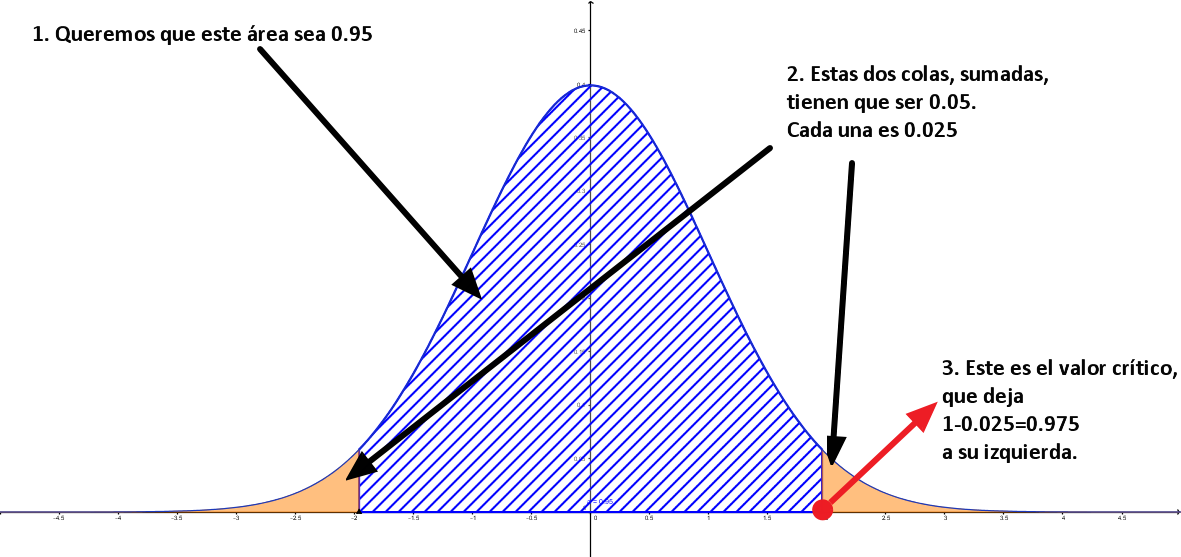
\includegraphics[width=16cm]{../fig/Tut06-08-IntervaloConfianzaz.png}
    \end{center}
Esta cuenta, el hecho de que empezamos con $0.95$, pero terminamos preguntando por el valor $0.975$ es de las que, inicialmente, más dificultades causan. Con la práctica, y dibujando siempre lo que queremos, las cosas irán quedando más y más claras.

Vamos a continuación a ver cómo calcular ese valor $z_{\alpha/2}=z_{0.025}$, y los correspondientes intervalos de confianza, usando R y algunos otros programas. Nuestra recomendación es que te acostumbres a usar R.

\subsection{Usando la función {\tt qnorm de } R.}
\label{tut06:subsec:IntConfMediaZConQnorm}

Para calcular el valor $z_{\alpha/2}=z_{0.025}$ en R, basta con ejecutar el comando:
\begin{knitrout}
\definecolor{shadecolor}{rgb}{0.969, 0.969, 0.969}\color{fgcolor}\begin{kframe}
\begin{alltt}
    \hlkwd{qnorm}\hlstd{(}\hlnum{0.975}\hlstd{)}
\end{alltt}
\begin{verbatim}
## [1] 1.96
\end{verbatim}
\end{kframe}
\end{knitrout}
Pero esta forma de proceder tiene el inconveniente de que nos obliga a hacer nosotros mismos la cuenta desde el nivel de confianza $nc=0.95$ hasta ese valor $1-\alpha/2=0.975$. Si cambiamos el nivel de confianza a $nc=0.90$ tenemos que repetir las cuentas, y corremos el riesgo de equivocarnos en algún paso. Es mejor automatizar, así que haremos que R haga toda la cuenta por nosotros:
\begin{knitrout}
\definecolor{shadecolor}{rgb}{0.969, 0.969, 0.969}\color{fgcolor}\begin{kframe}
\begin{alltt}
    \hlstd{nc}\hlkwb{=}\hlnum{0.95}
    \hlstd{(alfa}\hlkwb{=}\hlnum{1}\hlopt{-}\hlstd{nc)}
\end{alltt}
\begin{verbatim}
## [1] 0.05
\end{verbatim}
\begin{alltt}
    \hlstd{(alfa2}\hlkwb{=}\hlstd{alfa}\hlopt{/}\hlnum{2}\hlstd{)}
\end{alltt}
\begin{verbatim}
## [1] 0.025
\end{verbatim}
\begin{alltt}
    \hlstd{(z_alfa2}\hlkwb{=}\hlkwd{qnorm}\hlstd{(}\hlnum{1}\hlopt{-}\hlstd{alfa2) )}
\end{alltt}
\begin{verbatim}
## [1] 1.96
\end{verbatim}
\end{kframe}
\end{knitrout}
También podrías usar {\tt qnorm} con la opción {\tt lower.tail = FALSE}. Es en el fondo una cuestión de gustos.

Usando este tipo de código, es muy fácil elaborar un fichero con todas las instrucciones necesarias para automatizar casi por completo la tarea de calcular el intervalo de confianza. Hay dos casos posibles, que hemos visto en las Secciones \ref{curso-cap06:sec:IntervaloConfianzaMediaPoblacionNormal} y \ref{curso-cap06:sec:DesviacionTipicaMuestral} del libro:
\begin{itemize}
  \item Cuando podemos suponer que $X$ es normal y la varianza de la población es conocida, la fórmula del intervalo es (Ecuación \ref{curso-cap06:ecu:IntervaloConfianzaMediaSigmaConocida}, pág. \pageref{curso-cap06:ecu:IntervaloConfianzaMediaSigmaConocida} del libro):
      \[
        \bar X-z_{\alpha/2}\dfrac{\sigma_X}{\sqrt{n}}\leq \mu_X \leq \bar X+z_{\alpha/2}\dfrac{\sigma_X}{\sqrt{n}}.
      \]

  \item Si la varianza de la población es desconocida, pero el tamaño de la muestra es grande (en
      este curso estamos usando $n>30$), entonces la fórmula del intervalo es (Ecuación
      \ref{curso-cap06:ecu:EstadisticoMediaMuestralSigmaDesconocidaMuestraGrande}, pág.
      \pageref{curso-cap06:ecu:IntervaloConfianzaMediaMuestraGrande} del libro):
       \[
       \bar X-z_{\alpha/2}\dfrac{s}{\sqrt{n}}\leq \mu_X \leq \bar X+z_{\alpha/2}\dfrac{s}{\sqrt{n}}.
       \]

\end{itemize}
Las expresiones de ambos intervalos son muy parecidas, simplemente hay que cambiar $\sigma$ por $s$. Así que, {\bf teniendo siempre en cuenta las condiciones teóricas}, podemos usar el mismo código R para ambos casos. el código es muy simple, porque no hay que tomar decisiones: introducimos los datos del problema, y calculamos por orden todos los ingredientes del intervalo.

Pero todavía debemos tener en cuenta otro detalle: cómo recibimos los datos de la muestra. Podemos haber recibido la muestra {\em en bruto}, como un vector de datos (por ejemplo, en un fichero de tipo {\tt csv}), o podemos tener directamente los valores $\bar X$, $n$, $s$, etc. Esta última situación es típica de los {\em problemas de libro de texto}, mientras que la primera es una situación más frecuente en los que llamaremos {\em problemas del mundo real}, en los que los datos no vienen preparados.

En consecuencia, vamos a presentar dos ficheros {\em ``plantilla''}, uno para cada una de estas situaciones. El código está en los ficheros:
\begin{center}
\fichero{./code/Tut06-IntConf-Media-UsandoZ-Estadisticos.R}{Tut06-IntConf-Media-UsandoZ-Estadisticos.R}
\end{center}
y
\begin{center}
\fichero{./code/Tut06-IntConf-Media-UsandoZ-MuestraEnBruto.R}{Tut06-IntConf-Media-UsandoZ-MuestraEnBruto.R}
\end{center}
que aparecen en las Tablas \ref{tut05:tabla:Tut06-IntConf-Media-UsandoZ-Estadisticos.R} y \ref{tut05:tabla:Tut06-IntConf-Media-UsandoZ-MuestraEnBruto.R}, respectivamente. Échales un vistazo antes de seguir leyendo.

Cuando vayas a utilizar estos ficheros, especialmente las primeras veces, lee atentamente las instrucciones que aparecen en los comentarios. En particular,
\begin{itemize}
  \item Los ficheros {\bf no funcionarán} si no introduces toda la información en las líneas adecuadas de la primera parte del código. Para ayudarte a identificar donde termina la parte del fichero en la que tienes que introducir esa información, hemos incluido un bloque comentado en el código con este aspecto.
\begin{knitrout}
\definecolor{shadecolor}{rgb}{0.969, 0.969, 0.969}\color{fgcolor}\begin{kframe}
\begin{alltt}
  \hlcom{################################################}
  \hlcom{# NO CAMBIES NADA DE AQUI PARA ABAJO}
  \hlcom{################################################}
\end{alltt}
\end{kframe}
\end{knitrout}
  \item En el segundo de estos ficheros, el que trabaja con datos {\em en bruto}, existen, a su vez, dos posibilidades:
      \begin{itemize}
        \item Usar como punto de partida un vector de datos de R.
        \item Usar como punto de partida un fichero de datos, por ejemplo de tipo {\tt csv}.
      \end{itemize}
      Para indicarle a R cuál de esas dos posibilidades queremos utilizar {\bf es necesario} comentar (usando \verb/#/) la(s) línea(s) que no vamos a usar, e introducir la información necesaria en las líneas de la opción que sí usamos.
  \item En cualquier caso, es esencial tener en cuenta las {\bf condiciones teóricas de aplicabilidad} de estos ficheros. Para empezar, se supone que la población es normal. Pero incluso así, si la muestra es pequeña (pongamos $n < 30$) y no conoces $\sigma$, entonces {\bf no debes usar estos ficheros}.
  \item Para usar estos ficheros, no utilices {\em copiar y pegar} a partir de este pdf. Descarga los ficheros adjuntos en tu ordenador y ábrelos directamente con RStudio.
\end{itemize}

\begin{table}[p]
\lstinputlisting[numbers=none, language=R]{./code/Tut06-IntConf-Media-UsandoZ-Estadisticos.R}
\caption{Código R del fichero \fichero{./code/Tut06-IntConf-Media-UsandoZ-Estadisticos.R}{Tut06-IntConf-Media-UsandoZ-Estadisticos.R}}
\label{tut05:tabla:Tut06-IntConf-Media-UsandoZ-Estadisticos.R}
\end{table}

\begin{table}[p]
\lstinputlisting[numbers=none, basicstyle=\small ]{./code/Tut06-IntConf-Media-UsandoZ-MuestraEnBruto.R}
\caption{Código R del fichero \fichero{./code/Tut06-IntConf-Media-UsandoZ-MuestraEnBruto.R}{Tut06-IntConf-Media-UsandoZ-MuestraEnBruto.R}}
\label{tut05:tabla:Tut06-IntConf-Media-UsandoZ-MuestraEnBruto.R}
%\centering ¡¡Continúa en la siguiente página!!
\end{table}
Para que puedas practicar el funcionamiento de estos ficheros, aquí tienes un ejercicio con unos cuantos apartados, que cubren, esencialmente, todas las situaciones en las que te puedes encontrar.

\begin{ejercicio}
\label{tut06:ejercicio06}
%{\bf (Continúan en la página \pageref{tut06:parag:continuacionEjercicio06}.)}
\begin{enumerate}
  \item[]

  \item Una muestra de $n= 10$ elementos de una población normal con desviación típica conocida $\sigma=2.3$, tiene media muestral $\bar X=132.5$. Calcula intervalos  de confianza al 90\%, 95\% y 99\% para la media $\mu$. ¿Cómo son las anchuras de esos intervalos?

  \item Una muestra de $10$ elementos de una población normal tiene cuasidesviación típica $s=2.3$, y media muestral $\bar X=132.5$. Calcula un intervalo  de confianza al 95\% para la media $\mu$.

  \item Una muestra de $n = 450$ elementos de una población normal tiene cuasidesviación típica $s=2.3$, y media muestral $\bar X=132.5$. Calcula un intervalo de confianza al 99\% para la media $\mu$.

%  \newpage
%  \subsubsection*{}\label{tut06:parag:continuacionEjercicio06}
%  \item[] {\bf Continuación del Ejercicio \ref{tut06:ejercicio06}, pág. \pageref{tut06:ejercicio06}.}
  \item Dado este vector de datos,
\begin{knitrout}
\definecolor{shadecolor}{rgb}{0.969, 0.969, 0.969}\color{fgcolor}\begin{kframe}
\begin{alltt}
\hlstd{datos} \hlkwb{=} \hlkwd{c}\hlstd{(}\hlnum{3.09}\hlstd{,}\hlnum{3.06}\hlstd{,}\hlnum{2.79}\hlstd{,}\hlnum{2.44}\hlstd{,}\hlnum{2.54}\hlstd{,}\hlnum{3.52}\hlstd{,}\hlnum{3.07}\hlstd{,}\hlnum{2.67}\hlstd{,}\hlnum{2.99}\hlstd{,}\hlnum{2.82}\hlstd{,}\hlnum{2.94}\hlstd{,}\hlnum{3.57}\hlstd{,}\hlnum{2.38}\hlstd{,}\hlnum{3.24}\hlstd{,}
\hlnum{3.16}\hlstd{,}\hlnum{3.45}\hlstd{,}\hlnum{3.24}\hlstd{,}\hlnum{2.97}\hlstd{,}\hlnum{3.39}\hlstd{,}\hlnum{2.97}\hlstd{,}\hlnum{2.68}\hlstd{,}\hlnum{2.91}\hlstd{,}\hlnum{2.84}\hlstd{,}\hlnum{3.15}\hlstd{,}\hlnum{3.15}\hlstd{)}
\end{alltt}
\end{kframe}
\end{knitrout}
  del que sabemos que procede de una población normal con $\sigma=0.5$, calcula un intervalo de confianza al 95\% para la media $\mu$ de esa población.

  \item El fichero adjunto \fichero{../datos/Tut06-IntConf-Media-UsandoZ-datos.csv}{Tut06-IntConf-Media-UsandoZ-datos.csv} contiene una muestra de cierta población. Utiliza esos datos para calcular un intervalos  de confianza al 95\% para la media $\mu$ de esa población.

  \item Usa R para comprobar los resultados del Ejemplo \ref{curso-cap06:ejem:IntConfMediaSigmaConocida} del libro (pág. \pageref{curso-cap06:ejem:IntConfMediaSigmaConocida}).

\end{enumerate}
Soluciones en la página \pageref{tut06:ejercicio06:sol}.
\qed
\end{ejercicio}

\newpage

\subsection{Otros programas.}
\label{tut06:subsec:IntConfMediaZOtrosProgramas}
Vamos a ver brevemente las herramientas que nos ofrecen otros programas pra calcular intevalos de confianza para $\mu$, usando $Z$.

\subsubsection*{GeoGebra.}

En GeoGebra disponemos, en primer lugar, de la función
  \begin{center}
    \verb&IntervaloMediaZ[ <Media (muestra)>, <&$\sigma$\verb&>, <Tamaño (muestra)>, <Nivel> ]&
  \end{center}
donde los nombres de los argumentos entre los símbolos {\tt <} y {\tt >} indican en que orden debemos introducir los datos del problema. Por ejemplo, para obtener el intervalo de confianza del apartado 3 del Ejercicio \ref{tut06:ejercicio06} usaríamos la función de esta manera (en la {\em Línea de entrada}):
  \begin{verbatim}
    IntervaloMediaZ[132.5, 2.3, 450, 0.99]
  \end{verbatim}
y GeoGebra contesta con una {\em lista}, que contiene los dos extremos del intervalo.

Si lo que tenemos es un vector de datos, con un número no demasiado grande de elementos, podemos usar esta misma función de otra manera, siguiendo esta sintaxis:
  \begin{center}
    \verb&IntervaloMediaZ[ <Lista de datos (muestra)>, <&$\sigma$\verb&>, <Nivel> ]&
  \end{center}
Para ver como funciona, usaremos como ejemplo el apartado 4 del Ejercicio \ref{tut06:ejercicio06}. En primer lugar, creamos una lista en GeoGebra con los datos del problema, ejecutando este comando (tendrás que copiar cada línea por separado, para pegarlas formando  una única línea de entrada en GeoGebra):
  \begin{verbatim}
    datos = {3.09, 3.06, 2.79, 2.44, 2.54, 3.52, 3.07, 2.67, 2.99, 2.82, 2.94, 3.57,
    2.38, 3.24, 3.16, 3.45, 3.24, 2.97, 3.39, 2.97, 2.68, 2.91, 2.84, 3.15, 3.15}
  \end{verbatim}
Una vez hecho esto, calculamos el intervalo mediante:
\begin{verbatim}
    IntervaloMediaZ[datos, 0.5, 0.95]
\end{verbatim}
Como puedes ver, es difícil utilizar de forma práctica esta función cuando partimos de los datos {\em en bruto} de una muestra grande.
\begin{ejercicio}
\label{tut06:ejercicio07}
Usa GeoGebra para hacer el apartado 1 del Ejercicio \ref{tut06:ejercicio06}. Solución en la página \pageref{tut06:ejercicio07:sol}.
\qed
\end{ejercicio}

\subsubsection*{Interpretación probabilística del intervalo de confianza, usando GeoGebra.}
\label{tut06:subsubsec:InterpretacionProbabilisticaIntConfGeoGebra}

Antes de pasar a otros programas, queremos señalar que la Figura \ref{curso-cap06:fig:InterpretacionProbabilisticaIntervalosConfianza} del libro (pág. \pageref{curso-cap06:fig:InterpretacionProbabilisticaIntervalosConfianza}), que ilustra la interpretación probabilística de los intervalos de confianza, se ha obtenido con este fichero de GeoGebra:
\begin{center}
  \fichero{../ggb/Tut06-InterpretacionIntervalosConfianza.ggb}{Tut06-InterpretacionIntervalosConfianza.ggb}
\end{center}
Al abrirlo verás una ventana de GeoGebra similar a la de esta figura:
    \begin{center}
        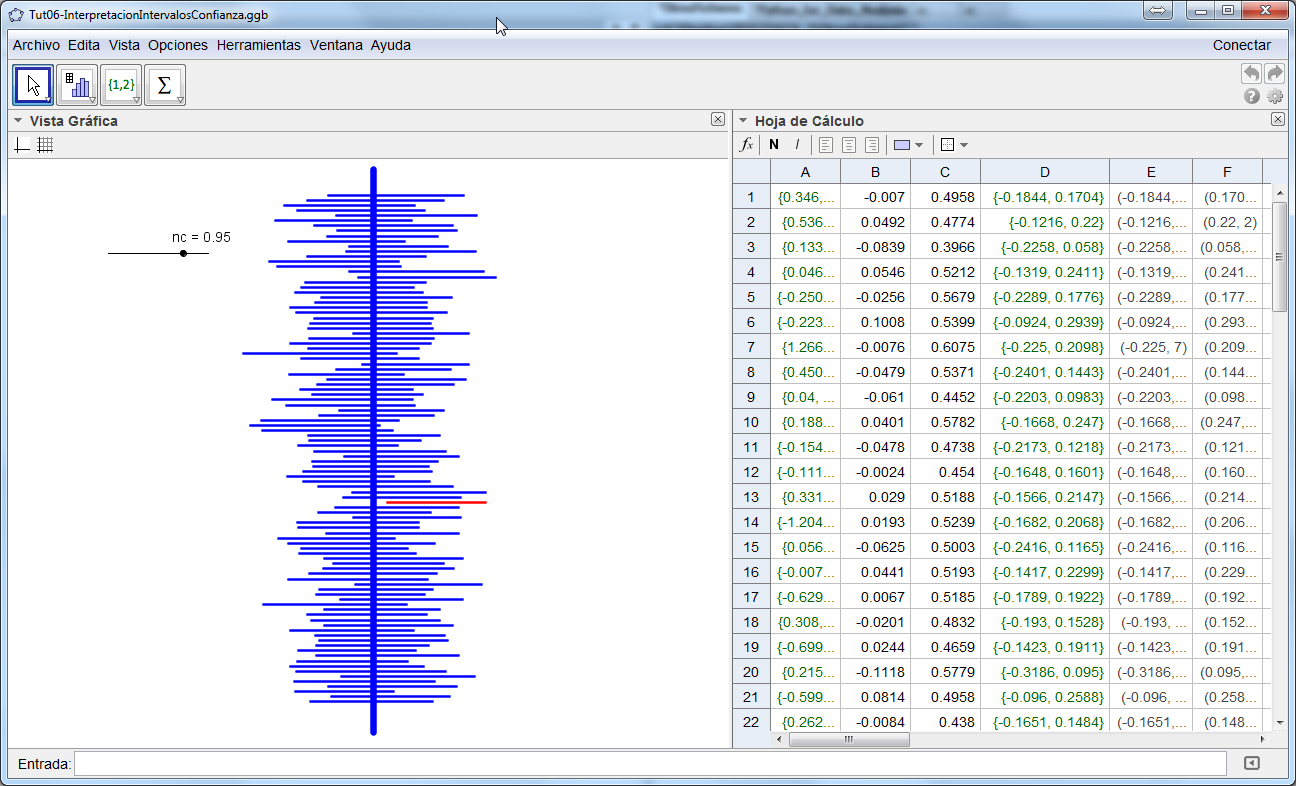
\includegraphics[width=15.5 cm]{../fig/Tut06-19.png}
    \end{center}
La parte izquierda contiene la {\em Vista Gráfica}, con una colección de $100$ intervalos de confianza, correspondientes a $100$ muestras distintas extraídas todas de la misma población normal. La parte derecha es la {\em Vista de hoja de cálculo}. Esta parte de GeoGebra tiene un comportamiento similar al de una hoja de cálculo como Calc. La diferencia fundamental es que las celdas de esta hoja de cálculo pueden guardar objetos geométricos, funciones, etc. Por ejemplo, puedes tener una columna llena de parábolas, por decir algo. En nuestro caso, la columna {\tt A} contiene las $100$ muestras, las columnas {\tt B} y {\tt C} contienen, respectivamente, las medias y cuasidesviaciones típicas de esas muestras y la columna {\tt D} contiene los intervalos de confianza. El resto de columnas contienen operaciones auxiliares para dibujar el gráfico, y aquí no nos detendremos en comentarlas.

Prueba a pulsar {\tt Ctrl + R} varias veces seguidas. Cada vez que lo haces, GeoGebra genera $100$ nuevos intervalos de confianza. Verás, destacados en color rojo, aquellos intervalos de confianza que no contienen a la media real de la población $\mu$, cuyo valor es $0$ y cuya posición se indica mediante el segmento vertical. Si el nivel de confianza es del $95\%$, es previsible que aparezcan alrededor de $5$ intervalos rojos. Tal vez alguno más, o alguno menos. Pero lo que significa ese nivel de confianza es que si tomamos muchas muestras, el $95\%$ de los intervalos de confianza correspondientes a esas muestras serán intervalos azules, de los que contienen a la media real de la población. Si lo deseas, puedes hacer clic con el botón derecho del ratón sobre cualquiera de los intervalos de la figura, y GeoGebra te indicará el número de fila que corresponde a ese intervalo concreto. Con ese número de fila puedes localizar el intervalo en la columna {\tt D} de la {\em Hoja de Cálculo}. Si el intervalo es rojo, podrás comprobar que $\mu=0$ no pertenece al intervalo, y a la recíproca en el caso de intervalos azules.

\subsubsection*{Wolfram Alpha.}
\label{tut06:subsubsec:IntConfMediaZWolframAlpha}

Para calcular intervalos de confianza como estos con Wolfram Alpha prueba a introducir  esta frase en el campo de entrada del programa:
\begin{verbatim}
    confidence interval for population mean
\end{verbatim}
Al hacerlo Wolfram Alpha abre una página con una serie de campos en los que podemos introducir los valores necesarios para la construcción del intervalo. La siguiente figura muestra esa página, en la que hemos introducido los valores correspondientes al apartado 1 del Ejercicio\ref{tut06:ejercicio06}. También se muestra el resultado que ha producido Wolfram Alpha.
    \begin{center}
        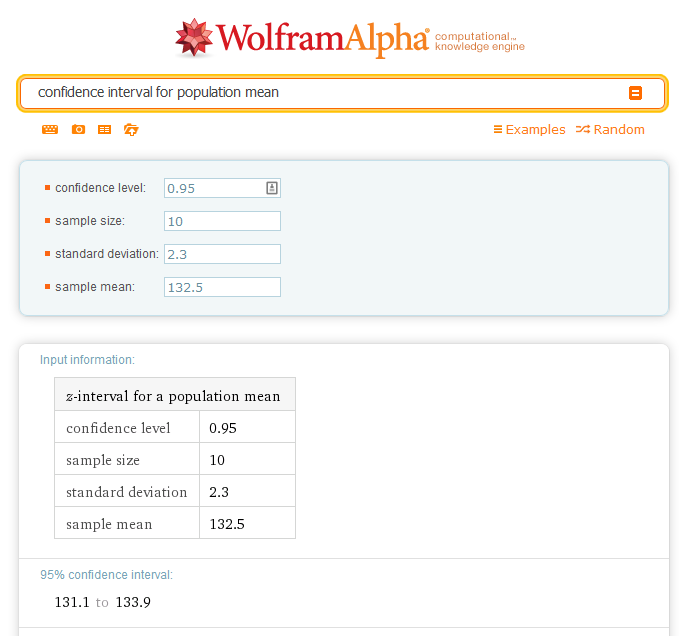
\includegraphics[width=15cm]{../fig/Tut06-18.png}
    \end{center}
En la versión gratuita de Wolfram Alpha que estamos usando no hay opciones para calcular un intervalo de confianza a partir de una muestra {\em en bruto} (esas opciones sí existen en la versión de pago).
Alternativamente, también puedes obtener el intervalo de confianza para la media usando un comando como este (es un ejemplo de la propia Web de Wolfram Alpha):
\begin{verbatim}
    z-interval mean 27, standard deviation 9,  sample size 100
\end{verbatim}
El resultado $(25.24,28.76)=27\pm 1.76397$, se muestra en una ventana como la que hemos visto arriba.
%    \begin{center}
%    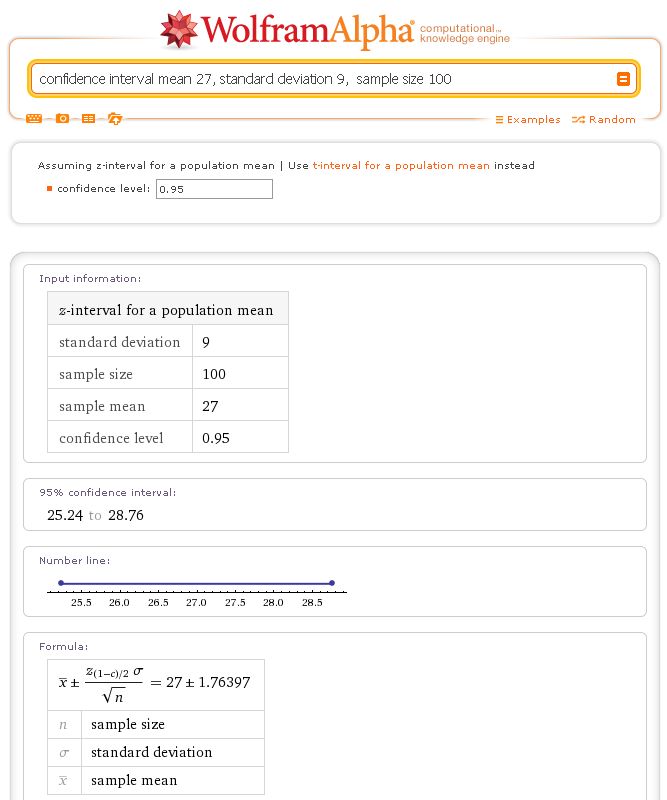
\includegraphics[height=10cm]{../fig/Tut06-15.png}
%    \end{center}
%

\subsubsection*{Calc.}
\label{tut06:subsubsec:IntConfMediaZCalc}

En Calc, para calcular los cuantiles de la distribución normal estándar $Z$ disponemos de la función
\begin{verbatim}
    DISTR.NORM.ESTAND.INV
\end{verbatim}
En la siguiente figura puedes ver el cuadro de diálogo correspondiente a esta función, que hemos ilustrado en el caso del cálculo de $z_{\alpha/2}$, para un nivel de confianza $nc=0.95$. Calc utiliza, en este caso al igual que R, la cola izquierda de $Z$.

Hemos indicado con las dos flechas rojas el valor de probabilidad (de la cola izquierda) que hemos introducido, y la respuesta que Calc va a producir. A partir de esta función es muy fácil elaborar una hoja de Calc que nos permita automatizar el cálculo del intervalo de confianza a partir de los datos de una muestra, como hemos hecho en el fichero:
\begin{center}
\fichero{../ods/Tut06-IntConf-Media-UsandoZ.ods}{Tut06-IntConf-Media-UsandoZ.ods}
\end{center}

\begin{center}
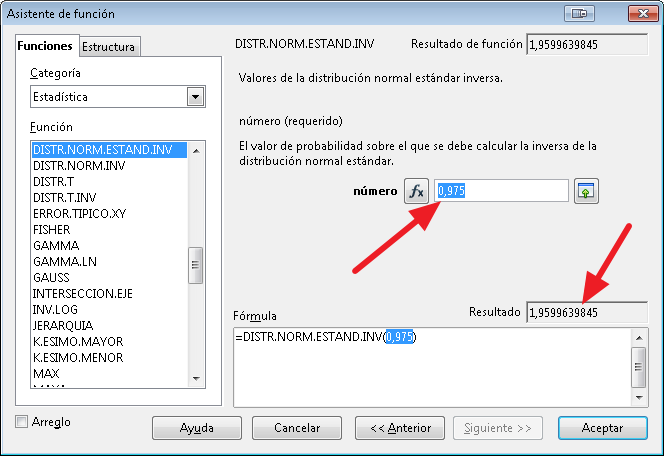
\includegraphics[width=14cm]{../fig/Tut06-09.png}
\end{center}
\vspace{3mm}

\begin{ejercicio}
\label{tut06:ejercicio08}
Usa este fichero para tratar de calcular los intervalos de confianza de los apartados 1 y 3 del Ejercicio \ref{tut06:ejercicio06} (pág. \pageref{tut06:ejercicio06}). ¿Qué dificultades encuentras? Solución en la página \pageref{tut06:ejercicio08:sol}.
\qed
\end{ejercicio}



Antes de seguir adelante, vamos a aprovechar nuestro paso por aquí para comentar los recursos que Calc ofrece para trabajar con distribuciones normales, tanto para problemas directos como inversos. Ya hemos comentado la función {\tt DISTR.NORM.ESTAND.INV}. Pero, además de esta, en Calc disponemos de las siguientes funciones:

\begin{itemize}
  \item {\tt DISTR.NORM.INV}. Sirve para problemas {\em inversos} en distribuciones normales no necesariamente iguales a $Z$. En la siguiente figura puedes ver el cuadro de diálogo en el que estamos usando esta función para resolver el problema inverso:
      \[P(X<K) = 0.8, \]
      en una normal $X$ de tipo $N(\mu=6.3, \sigma=0.23)$. Usamos
      {\tt DISTR.NORM.INV(0,80;6,3;0,23)} para obtener $6.4935728837$.
            \begin{center}
            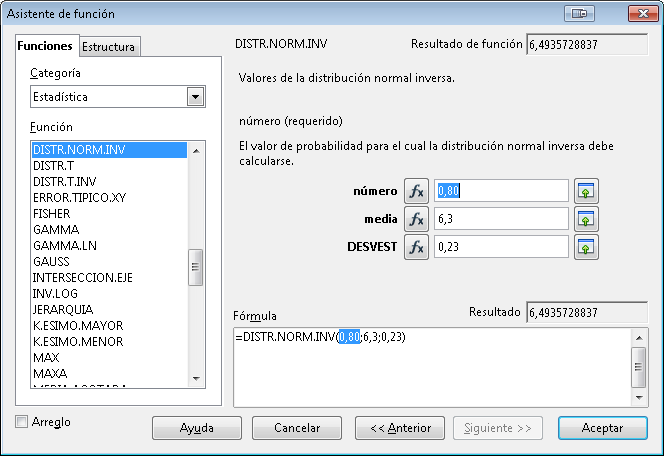
\includegraphics[width=13.52cm]{../fig/Tut06-10.png}
            \end{center}

  \item {\tt DISTR.NORM}. Sirve para problemas {\em directos} en distribuciones normales no necesariamente iguales a $Z$. La siguiente figura muestra el cuadro de diálogo en el que estamos usando esta función para resolver el problema directo:
      \[P(X<4.2) = ??, \]
      en una normal $X$ de tipo $N(\mu=3.2, \sigma=1.15)$. Usamos {\tt DISTR.NORM(4,2;3,2;1,15;1)} para obtener $0,8077309735$.
            \begin{center}
            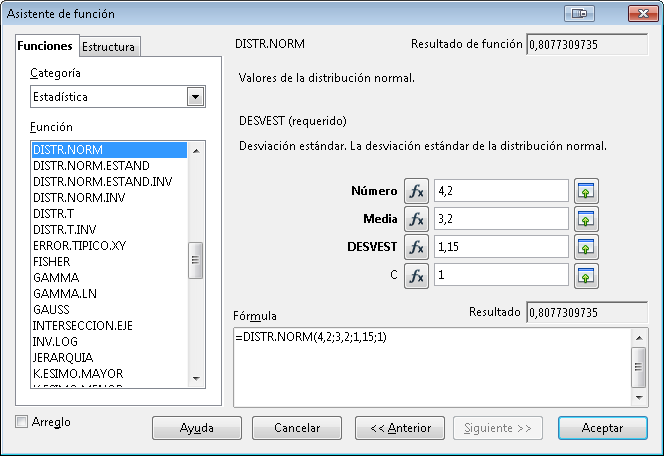
\includegraphics[width=13.5cm]{../fig/Tut06-11.png}
            \end{center}
      En el caso de esta función debemos introducir un parámetro adicional, que Calc llama {\tt C}, que puede ser $C=1$ o $C=0$. El valor $C=1$ sirve para calcular la función de distribución de la normal (como {\tt pnorm} en R, y también con la cola izquierda). El valor $C=0$ devuelve valores de la función de densidad de la normal (como {\tt dnorm} en R), y apenas lo vamos a utilizar en este curso.

  \item {\tt DISTR.NORM.ESTAND} Finalmente, esta función se usa para problemas {\em directos} en la distribución normal estándar $Z$. En este caso siempre se calcula la función de distribución ({\tt pnorm}, cola izquierda), y el único argumento es el valor del que sea calcular la probabilidad de su cola izquierda. Por ejemplo, para resolver
      \[P(Z<2.1)\]
      usaríamos {\tt DISTR.NORM(2,1)} para obtener $0,9821355794$.
\end{itemize}


\section{Muestras pequeñas. La $t$ de Student.}
\label{tut06:sec:IntervalosConfianzaMediaStudent}

En esta sección vamos a ver cómo utilizar los programas que conocemos para trabajar en problemas en los que interviene la distribución $t$ de Student.

\subsection{Relación entre la $t$ de Student y la normal $Z$, usando GeoGebra.}
\label{tut06:subsec:RelacionStudentZUsandoGeoGebra}

Al principio de la Sección \ref{curso-cap06:sec:tStudent} del libro hemos explicado que si $T_k$ es una distribución tipo $t$ de Student,  con $k$ grados de libertad, entonces a medida que $k$ aumenta la distribución se parece cada vez más a la normal estándar $Z$, de manera que a partir de $k=30$ las gráficas de las densidades de ambas distribuciones son prácticamente idénticas. Para ilustrar esto te hemos preparado un fichero GeoGebra muy sencillo:
\begin{center}
  \fichero{../ggb/Tut06-ZvsT.ggb}{Tut06-ZvsT.ggb}
\end{center}
Al abrirlo verás algo como esto:
  \begin{center}
        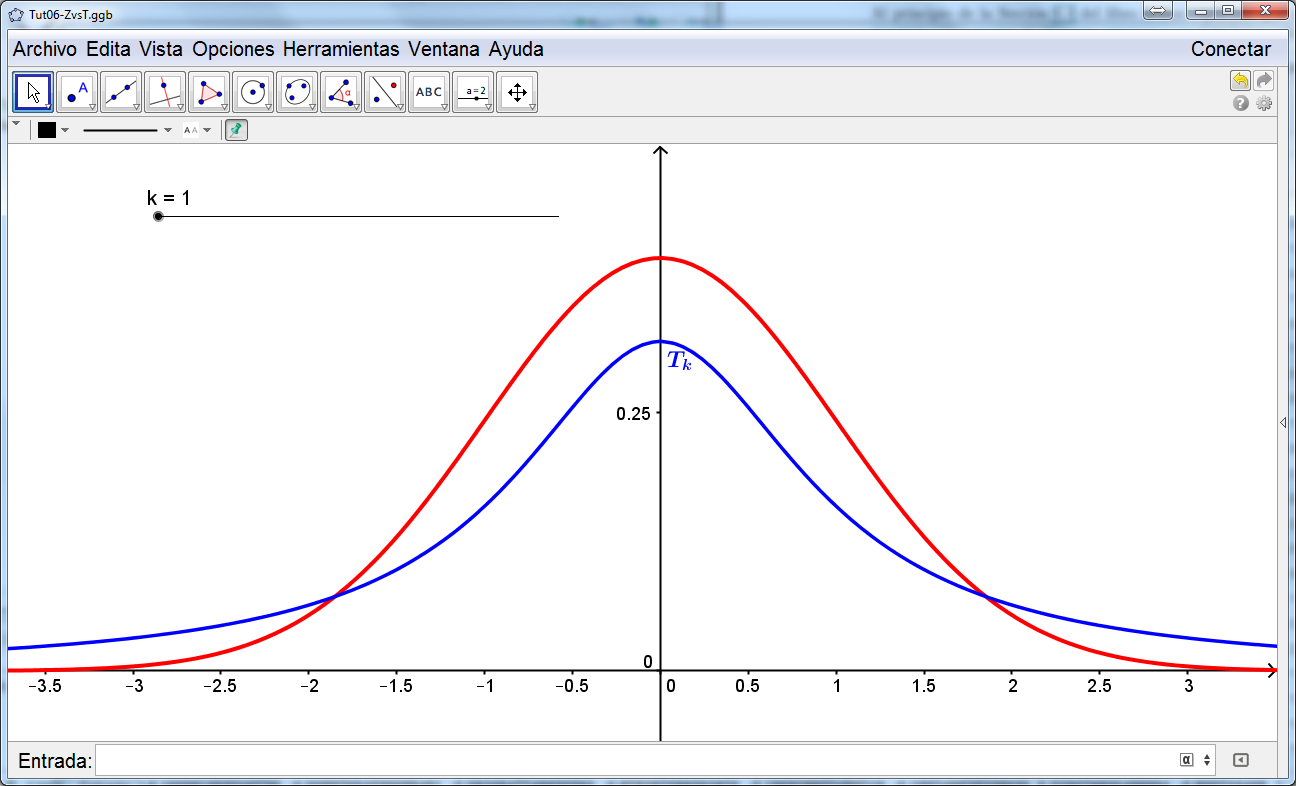
\includegraphics[width=14cm]{../fig/Tut06-28.png}
  \end{center}


El fichero muestra las dos funciones de densidad, $Z$ en rojo y $T_k$ en azul, y un deslizador que permite ir variando el valor de $k$, entre $1$ y $100$, para que puedas ver lo que sucede. Para dibujar las dos curvas hemos usado estos comandos de GeoGebra:
\begin{verbatim}
  DistribuciónT[k, x ]
  Normal[0, 1, x ]
\end{verbatim}

\subsection{Cálculos de probabilidad para la $t$ de Student en R.}
\label{tut06:subsec:CalculosProbabilidadtStudentConR}

Una ventaja de trabajar con R, como ya hemos comentado anteriormente, es la homogeneidad en la sintaxis para todas las distribuciones de probabilidad. Concretamente, el trabajo con la $t$ de Student es prácticamente igual al que hemos visto con la normal estándar $Z$, salvo por el detalle de los grados de libertad. Si en el caso de $Z$ teníamos las funciones {\tt dnorm}, {\tt pnorm}, {\tt qnorm}, y {\tt rnorm}, ahora tenemos sus análogas {\tt dt}, {\tt pt}, {\tt qt} y {\tt rt}, con los significados evidentes. La primera de ellas, {\tt dt}, sirve para calcular la función de densidad, y apenas la usaremos. La última, {\tt rt}, permite calcular valores aleatorios, distribuidos según la $t$ de Student. La usaremos sobre todo para hacer simulaciones. Las dos restantes, {\tt pt} y {\tt qt} llevarán el peso de nuestro trabajo con esta distribución. Vamos a presentarlas brevemente, antes de ponerlas a trabajar.

\subsubsection*{Las funciones {\tt pt} y {\tt qt}.}
\label{tut06:subsubsec:funcion_pt}

La función {\tt pt} calcula la probabilidad de la cola izquierda (como siempre) de una distribución $t$ de Student. Por ejemplo, si $T_{18}$ es una distribución $t$ de Student con $k=18$ grados de libertad, el problema directo de probabilidad:
\[P(T_{18} < 2.3)\]
se resuelve mediante este comando en R:
\begin{knitrout}
\definecolor{shadecolor}{rgb}{0.969, 0.969, 0.969}\color{fgcolor}\begin{kframe}
\begin{alltt}
\hlkwd{pt}\hlstd{(}\hlnum{2.3}\hlstd{,} \hlkwc{df} \hlstd{=} \hlnum{18}\hlstd{)}
\end{alltt}
\begin{verbatim}
## [1] 0.98319
\end{verbatim}
\end{kframe}
\end{knitrout}
Los grados de libertad se indican, como ves, con el argumento {\tt df} (del inglés {\em degrees of freedom}). Si deseas usar la cola derecha dispones, como siempre, de la opción {\tt lower.tail=FALSE}. Para calcular en una $T_{12}$ (es decir, una distribución $t$ de Student con $12$ grados de libertad) la probabilidad
\[P\left(T_{12}> 3.1 \right)\]
podemos usar indistintamente estos dos comandos:
\begin{knitrout}
\definecolor{shadecolor}{rgb}{0.969, 0.969, 0.969}\color{fgcolor}\begin{kframe}
\begin{alltt}
\hlnum{1} \hlopt{-} \hlkwd{pt}\hlstd{(}\hlnum{3.1}\hlstd{,} \hlkwc{df} \hlstd{=} \hlnum{12}\hlstd{)}
\end{alltt}
\begin{verbatim}
## [1] 0.004595
\end{verbatim}
\begin{alltt}
\hlkwd{pt}\hlstd{(}\hlnum{3.1}\hlstd{,} \hlkwc{df} \hlstd{=} \hlnum{12}\hlstd{,} \hlkwc{lower.tail}\hlstd{=}\hlnum{FALSE}\hlstd{)}
\end{alltt}
\begin{verbatim}
## [1] 0.004595
\end{verbatim}
\end{kframe}
\end{knitrout}

La función {\tt qt}, por su parte, permite calcular los cuantiles, y por tanto resolver problemas inversos de probabilidad asociados con la $t$ de Student. Como siempre, por defecto, se usa la cola izquierda de la distribución, salvo que usemos {\tt lower.tail=FALSE}. Es decir, que para resolver un problema como el de encontrar el valor $K$ tal que
\[P(T_{24} < K) = 0.87\]
usaríamos este comando de R:
\begin{knitrout}
\definecolor{shadecolor}{rgb}{0.969, 0.969, 0.969}\color{fgcolor}\begin{kframe}
\begin{alltt}
\hlkwd{qt}\hlstd{(}\hlnum{0.87}\hlstd{,} \hlkwc{df} \hlstd{=} \hlnum{24}\hlstd{)}
\end{alltt}
\begin{verbatim}
## [1] 1.1537
\end{verbatim}
\end{kframe}
\end{knitrout}

Vamos a practicar el uso de ambas funciones con unos cuantos ejercicios.

\begin{ejercicio}
\label{tut06:ejercicio09}
Sea $T_{15}$ una variable aleatoria de tipo $t$ de Student, con $k=15$ grados de libertad. Calcular los siguientes valores. {\bf Es muy recomendable} hacer un dibujo esquemático de la situación en cada uno de los apartados.
    \begin{enumerate}
        \item $P(T_{15}\leq -1.341)$
        \item $P(T_{15}\geq 2.602)$
        \item $P(-1.753\leq T_{15}\leq 1.753)$
        \item Valor de $t$ tal que $P(T_{15}\leq t)=0.95$.
        \item Valor de $t$ tal que $P(T_{15}\geq t)=0.025$.
        \item Valor de $t$ tal que $P(T_{15}\leq t)=0.05$.
        \item Valor de $t$ tal que $P(T_{15}\geq t)=0.975$.
        \item Valor de $t$ tal que $P(-t\leq T_{15}\leq t)=0.95$.
        \item Valor de $t$ tal que $P(-t\leq T_{15}\leq t)=0.93$.
    \end{enumerate}
Soluciones en la página \pageref{tut06:ejercicio09:sol}.
\qed
\end{ejercicio}
Los dos últimos apartados de este ejercicio son ejemplos del tipo de cálculo que necesitamos para obtener los valores críticos que se usan en un intervalo de confianza, como los que vamos a construir a continuación.

\subsection{La $t$ de Student en GeoGebra, Wolfram Alpha y Calc.}
\label{tut06:subsec:tStudentConR}

\subsubsection{GeoGebra.}

La {\em Calculadora de Probabilidades} de GeoGebra permite trabajar con la distribución $t$ de Student de forma muy parecida a lo que vimos en el caso de la distribución normal. Basta con seleccionar {\tt Student} en el menú desplegable que se sitúa bajo la gráfica.

Aparte de esto, puedes usar directamente algunas funciones en la {\em Línea de Entrada} de GeoGebra. Por ejemplo
\begin{verbatim}
    DistribuciónT[k, x]
\end{verbatim}
produce como resultado la probabilidad de la cola izquierda de $x$ en la distribución $T_k$:
\[P(T_k \leq x)\]
Es decir, el mismo efecto que si en R utilizaras $pt(x, df=k)$. Recuerda que los resultados se obtienen en el panel de {\em Vista Algebraica}, a la izquierda (si no es visible, usa el menú {\em Vista} para hacerlo aparecer).


En la versión actual de GeoGebra, para conseguir la probabilidad de una cola derecha hay que usar el truco de $1-p$. Es decir,
\begin{verbatim}
  1 - DistribuciónT[k, x]
\end{verbatim}
produce, como cabe esperar, el valor
\[P(T_k > x).\]
Para los problemas inversos de probabilidad disponemos de la función
\begin{verbatim}
  DistribuciónTInversa[k, p]
\end{verbatim}
cuyo resultado es el valor $x$ tal que:
\[P(T_k \leq x) = p.\]
Es decir el cuantil $p$ de $T_k$, que en R calcularíamos con {\tt qt(p, df=k)}. De nuevo, si deseas localizar el valor cuya cola derecha  representa una probabilidad $p$, usa un truco como:
\begin{verbatim}
  DistribuciónTInversa[k, 1- p]
\end{verbatim}

\begin{ejercicio}
\label{tut06:ejercicio10}
Usa estas funciones, o la {\em Calculadora de Probabilidades} de GeoGebra para repetir el Ejercicio \ref{tut06:ejercicio09}.
\qed
\end{ejercicio}

\subsubsection{Wolfram Alpha.}

La sintaxis de Wolfram Alpha es, como siempre, algo más peculiar. Seguramente existen otras formas de calcular estas cantidades, pero las que incluimos aquí son las más sencillas que conocemos.

Vamos a resolver, en primer lugar un problema directo de probabilidad. Concretamente, dada una distribución $T_{21}$, vamos a calcular la probabilidad:
\[P(T_{21}>2.7)\]
Para ello, en Wolfram Alpha ejecutamos el comando:
\begin{verbatim}
    P[X > 2.3] for X student t with 21 dof
\end{verbatim}
y obtenemos como resultado aproximado $0.0159011$. Si lo que deseas es la probabilidad de un intervalo, como en este ejemplo (procede de la propia página de Wolfram Alpha)
\[P(-1.2 < T_{12} < 2.3)\]
puedes usar una sintaxis como esta:
\begin{center}
\begin{verbatim}
    P[-1.2 < X < 2.3] for X student t with 12 dof
\end{verbatim}
\end{center}
y obtendrás el valor aproximado $0.853254$.

\begin{ejercicio}
\label{tut06:ejercicio11}
Usa R o GeoGebra (o, aún mejor, ambos) para comprobar estos resultados. Solución en la página \pageref{tut06:ejercicio11:sol}.
\qed
\end{ejercicio}

Los problemas inversos se pueden resolver reduciéndolos manualmente a problemas sobre la cola izquierda de la distribución $T_k$. Por ejemplo, para encontrar el valor $x$ tal que (es una cola derecha)
\[P(T_{12} > x) = 0.07\]
hacemos un pequeño esquema gráfico que nos ayude a entender que esto es lo mismo que buscar el valor $x$ tal que
\[P(T_{12} < x) = 0.93.\]
Y ahora podemos pedirle a Wolfram Alpha que nos diga cuál es ese valor usando esta sintaxis:
\begin{center}
  \begin{verbatim}
    93th percentile  for student t with 12 dof
  \end{verbatim}
\end{center}
El resultado aproximado es $1.5804$.

\begin{ejercicio}
\label{tut06:ejercicio12}
Usa R o GeoGebra (o, aún mejor, ambos) para comprobar este resultado. Solución en la página \pageref{tut06:ejercicio12:sol}.
\qed
\end{ejercicio}

\subsubsection{Calc.}
\label{tut06:subsubsec:StudentConCalc}

En Calc, las funciones {\tt DISTR.T} y {\tt DISTR.T.INV} permiten resolver problemas directos e inversos de probabilidad para la distribución $t$ de Student, de modo parecido a lo que hemos visto para la distribución normal. Pero es importante entender las diferencias. Empecemos, en este caso, por los problemas directos. El cuadro de diálogo que aparece, al utilizar la función {\tt DISTR.T} para resolver, usando la distribución $T_{3}$ (con $k=3$ grados de libertad) un problema directo, es este:
    \begin{center}
    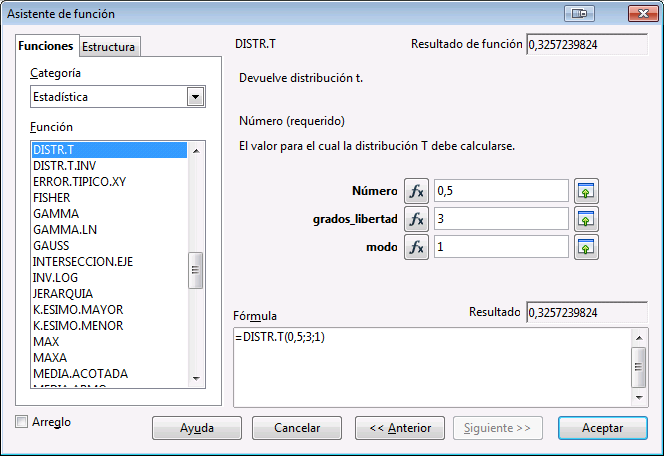
\includegraphics[width=15cm]{../fig/Tut06-13.png}
    \end{center}
La función tiene un parámetro {\tt modo}, que puede tomar los valores 1 o 2. Ese valor indica el número de colas de la distribución que se utilizan. Si ${\tt modo = 2}$, entonces Calc obtiene el resultado repartiendo la probabilidad entre las dos colas de la distribución $t$ (que es justo lo que se utiliza para construir el intervalo de confianza). Pero si ${\tt modo = 1}$, entonces Calc sólo utiliza una de las dos colas.

\begin{ejercicio}
\label{tut06:ejercicio13}
\begin{enumerate}
  \item[]
  \item Observa los datos del ejemplo que aparecen en ese cuadro de diálogo. Es decir,
    \begin{verbatim}
    Número = 0,5
    grados_libertad = 3
    modo = 1
    \end{verbatim}
    Y el resultado que es aproximadamente $0.3257$.  Teniendo en cuenta este ejemplo, ¿qué cola de la distribución $t$ usa Calc cuando {\tt modo = 1}? Una representación gráfica puede ayudarte con esta pregunta.
  \item Para confirmar que lo has entendido, usa R para calcular este mismo valor.
\end{enumerate}
Solución en la página \pageref{tut06:ejercicio13:sol}.
\qed
\end{ejercicio}

\quad\\
\vspace{1cm}
\begin{center}
\textcolor{red}{\bf\LARGE ¡No sigas, si no has hecho este ejercicio!}
\end{center}

\newpage

Puesto que la distribución $T$ tiene (como la normal estándar $Z$) una forma de campana simétrica, centrada en el 0, si tomamos un valor situado a la derecha del cero (como el $0,5$ del ejercicio), su cola derecha tiene que valer menos de $\frac{1}{2}$, y su cola izquierda más de $\frac{1}{2}$. Viendo el resultado de Calc en este ejemplo concluimos que (lamentablemente, desde nuestro punto de vista):
    \begin{center}
    \fcolorbox{black}{Gris025}{
    \begin{minipage}{12.5cm}
        \begin{center}
        La función  {\tt DISTR.T} de Calc, con {\tt modo = 1}, usa la \underline{\bf cola derecha} de la distribución $t$ de Student.
        \end{center}
    \end{minipage}}
    \end{center}
Es decir que el resultado de un comando como:
    \begin{center}
    {\tt DISTR.T(a; k; 1)}
    \end{center}
es
    \[P(T_k > a)\]
Si se usa $modo = 2$ se obtiene el área de ambas colas. Es decir, se calcula
\[P( T_k < -a) + P(T_k > a),\]
o, lo que es lo mismo, $P(|T_k| > a)$).

El ejemplo que hemos visto antes, con
    \[\mbox{\tt DISTR.T(0,5; 3; 1) = 0,3257239824}\]
corresponde al cálculo de:
\[P\left(T_3 > \frac{1}{2}\right),\]
que se ilustra en esta figura
    \begin{center}
    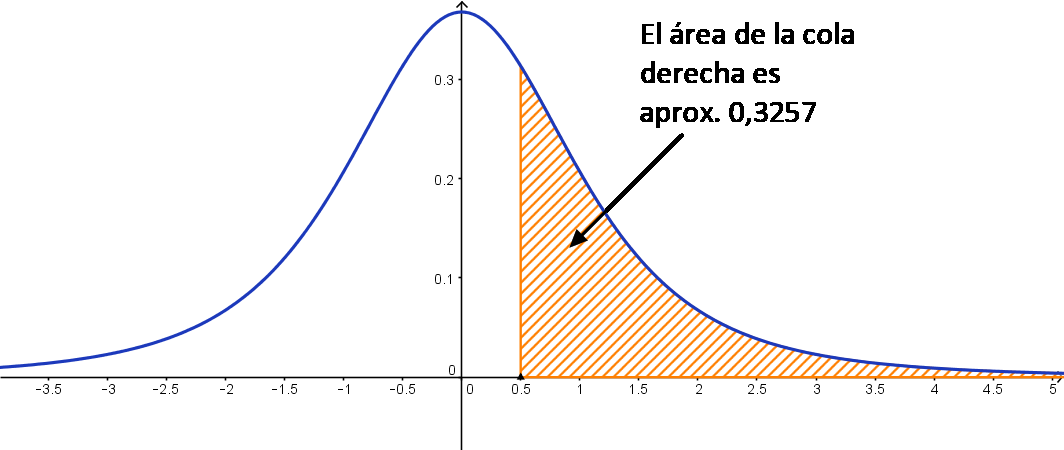
\includegraphics[width=14cm]{../fig/Tut06-12.png}
    \end{center}
Si lo que queremos es calcular una cola izquierda, como en $P(T_3 < \frac{1}{2})$, debemos utilizar el truco de $1 - p$:
    \[\mbox{\tt 1 - DISTR.T(0,5;3;1) = 0,6742760176}\]

Para los problemas inversos de probabilidad y, por lo tanto, para obtener los valores críticos necesarios para los intervalos de confianza, la hoja de cálculo incluye la función {\tt DISTR.T.INV}. Y aquí, de nuevo, hay que ir con cuidado, porque el resultado de
    \[\mbox{\tt DISTR.T.INV(p; k)}\]
es el valor $x$ tal que
    \[P(T_k < -x) + P(T_k > x)  = p,\]
Es decir:
    \begin{center}
    \fcolorbox{black}{Gris025}{
    \begin{minipage}{12.5cm}
        \begin{center}
         La función {\tt DISTR.T.INV} {\sf siempre usa el área de
         \underline{las dos colas, derecha e izquierda}}.
        \end{center}
    \end{minipage}}
    \end{center}
Por ejemplo, para calcular el $x$ tal que
    \[\underbrace{P(T_3 < -x)}_{\mbox{\tiny cola izda.}}+\underbrace{P(T_3 > x)}_{\mbox{\tiny cola dcha.}}=\frac{1}{2},\]
usamos
         \[\mbox{\tt DISTR.T.INV(0,5; 3) = 0,7648923284},\]
El problema se ilustra en esta figura
    \begin{center}
    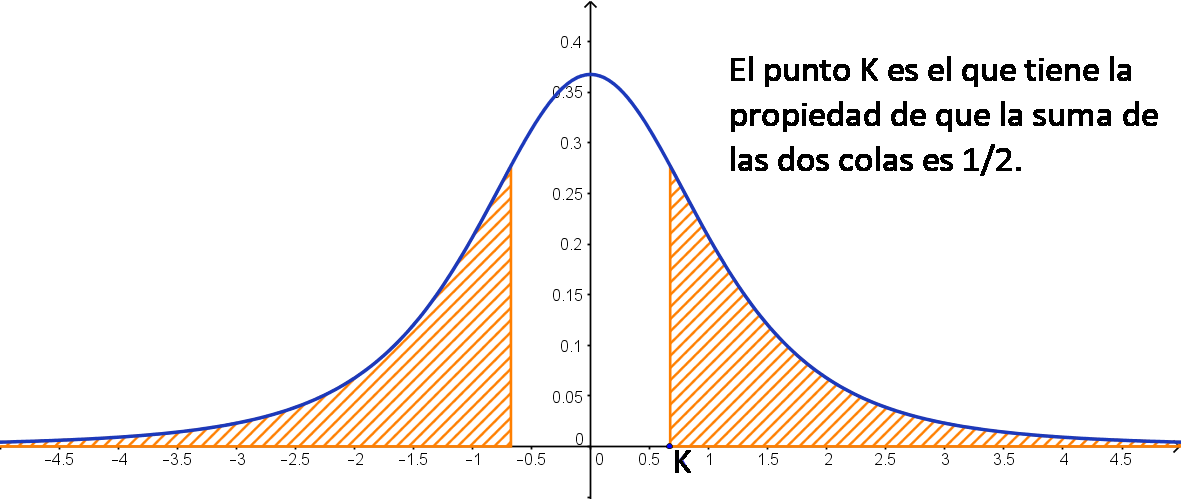
\includegraphics[width=15cm]{../fig/Tut06-14.png}
    \end{center}
A pesar de la confusión que, probablemente genera, la ventaja de esto es que, si lo que quiero es encontrar el valor crítico para construir un intervalo de confianza, entonces a partir del nivel de confianza $1-\alpha$, precisamente lo que necesitamos saber es cuál es el valor de $K$ tal que
    \[P(X>K)+P(X<-K)=\alpha\]
y eso, directamente, es lo que nos da {\tt DISTR.T.INV}. Por ejemplo, con $3$ grados de libertad, el valor crítico para un intervalo de confianza  para la media al $95\%$ (es decir $\alpha=0.05$), que es $t_{k;\alpha/2}=t_{3;0.025}$, se obtiene con
    \[\mbox{\tt DISTR.T.INV(0,05;3)=3,1824463053},\]


Como resumen final, nuestra opinión es que la falta de coherencia entre las distintas funciones de Calc (a veces cola izquierda, a veces derecha, a veces las dos...) aconseja ser muy prudentes a la hora de usar el programa. Afortunadamente, creemos haber presentado suficientes alternativas como para hacer esencialmente innecesario el uso de Calc en estos problemas.


\section{Intervalos de confianza para la media usando $t$.}
\label{tut06:sec:IntConfMediaUsandoT}

Empecemos recordando que la $t$ de Student se usa para calcular intervalos de confianza cuando se cumplen estas condiciones:
    \[\begin{cases}
     \mbox{(1) La población original es normal (o, al menos, aproximadamente normal).}\\[3mm]
     \mbox{(2) Desconocemos la varianza de la población $\sigma^2_X$}.\\[3mm]
     \mbox{(3) El tamaño de la muestra es pequeño ($n<30$ sirve de referencia).}
     \end{cases}
     \]
La fórmula del intervalo (Ecuación \ref{curso-cap06:ecu:IntervaloConfianzaMediaUsandoT} del libro, pág. \pageref{curso-cap06:ecu:IntervaloConfianzaMediaUsandoT}) es:
       \[
       \bar X-t_{k;\alpha/2}\dfrac{s}{\sqrt{n}}\leq \mu_X \leq \bar X+t_{k;\alpha/2}\dfrac{s}{\sqrt{n}}.
       \]
Es decir, es prácticamente igual a la del caso en que usábamos $Z$, pero sustituyendo $z_{\alpha/2}$ por $t_{k;\alpha/2}$ (donde $k = n-1$, recuérdalo).  En esta sección vamos a ver como usar distintos programas para calcular los intervalos de confianza en esos casos.

\subsection{Usando R, primera versión: ficheros plantilla.}
\label{tut06:subsec:IntConfMediaUsandoTConRPlantillas}

Para construir intervalos de confianza usando $t$ en R disponemos de dos ficheros ``plantilla'', casi idénticos a los que vimos para la normal:
\begin{center}
\begin{tabular}{ll}
Datos resumidos: & \fichero{./code/Tut06-IntConf-Media-UsandoT-Estadisticos.R}{Tut06-IntConf-Media-UsandoT-Estadisticos.R}\\[2mm]
Datos {\em en bruto}&
\fichero{./code/Tut06-IntConf-Media-UsandoT-MuestraEnBruto.R}{Tut06-IntConf-Media-UsandoT-MuestraEnBruto.R}
\end{tabular}
\end{center}
El primero de estos ficheros se usa para los ejercicios {\em `` de libro de texto''}, en los que en lugar de usar como punto de partida los datos de la muestra, disponemos de los valores de $n, \bar X$ y $s$, calculados previamente. El segundo, en cambio, es el adecuado cuando partimos de la muestra completa, en un vector de R, o en un fichero {\tt csv} en la página \pageref{tut06:subsubsec:CocinandoMuestras} veremos que esa diferencia no es tan relevante).

El uso de estos ficheros es prácticamente idéntico al que vimos en el caso en el que se usaba $Z$. La  única diferencia reseñable es que aquí {\em siempre} se va a usar $s$, la cuasidesviación típica muestral, porque se supone que desconocemos $\sigma$ (¡de otro modo usaríamos $Z$!). Lo mejor es, simplemente, practicar haciendo algunos ejercicios.

\begin{ejercicio}
\label{tut06:ejercicio14}
\begin{enumerate}
  \item[]
  \item El {\em ``ejercicio trampa''}, del apartado 2 del Ejercicio \ref{tut06:ejercicio06} (pág. \pageref{tut06:ejercicio06}). Una muestra de $10$ elementos de una población normal, tiene cuasidesviación típica $s=2.3$, y una media muestral $\bar X=132.5$. Calcula un intervalo  de confianza al $95\%$ para la media $\mu$.

  \item Los siguientes $15$ valores proceden de una población normal. Calcula un intervalo de confianza al $95\%$ para la media de esa población.
    \begin{verbatim}
    3.14, 3.71, 2.77, 4.08, 4.18, 1.51, 3.65, 3.41, 4.51, 2.27, 3.28,
    2.26, 2.80, 2.54, 3.77
    \end{verbatim}

  \item La $t$ de Student se usa (principalmente) con muestras pequeñas. Por esa razón puede que pienses que aprender a trabajar a partir de ficheros {\tt csv} no es, en este caso, tan necesario.  Para intentar persuadirte de que puede merecer la pena, aquí tienes un fichero {\tt csv} con $20$ valores procedentes de una distribución normal:
      \begin{center}
        \fichero{../datos/Tut06-DatosIntConfConStudent.csv}{Tut06-DatosIntConfConStudent.csv}
      \end{center}
      Usa R para calcular un intervalo de confianza al $95\%$ para estos datos.

Yo, desde luego, prefiero leer este fichero usando {\tt read.table} (y la opción \verb/dec=","/ para gestionar la coma como separador de decimales). De esa forma, los datos se leen en una sola línea de código en R, en lugar de hacer operaciones de {\em copia/pega}, reemplazar comas por puntos, etc.

  \item {\bf IMPORTANTE:} la distribución $t$ de Student es muy útil para trabajar con muestras pequeñas. Pero eso no significa que no pueda usarse con muestras grandes. Para ver lo que sucede, repite el apartado 3 del Ejercicio \ref{tut06:ejercicio06} (en el que $n=450$).

  \item Comprueba con R la solución del Ejemplo \ref{curso-cap06:ejem:IntConfMediaConTBacterias} del libro (pág. \pageref{curso-cap06:ejem:IntConfMediaConTBacterias}).

\end{enumerate}
Solución en la página \pageref{tut06:ejercicio14:sol}.
\qed
\end{ejercicio}

\subsection{Usando R, segunda versión: la función {\tt t.test} y similares.}
\label{tut06:subsec:IntConfMediaUsandoTConTtest}

Aparte de las plantillas que hemos descrito en la sección precedente, R incluye una función propia, la función {\tt t.test}, que puede usarse para calcular intervalos de confianza con la $t$ de Student.
En realidad, el objetivo principal de esta función es realizar un Contraste de Hipótesis, una técnica que se explica en el Capítulo \ref{curso-cap:ContrasteHipotesis} del libro. Cuando estudiemos ese tema volveremos a visitar esta función {\tt t.test} para conocerla con más detalle (y todavía tendremos ocasión de volver sobre ella más adelante en el curso). Pero, como aperitivo, aquí vamos a ver cómo se puede usar esta función para obtener el intervalo de confianza.

La función {\tt t.test}, como muchas otras funciones de R, está pensada para trabajar directamente sobre un vector de datos. El motivo por el que esto es así es que R se diseñó para un uso profesional, para tratar los que antes hemos llamado {\em problemas del mundo real}, para marcar la diferencia con los {\em problemas de libro de texto}. Recuerda que, en un {\em problema de libro de texto} partimos de los valores estadísticos ya calculados de la muestra ($n$, $\bar X$, $s$).  Pero en un {\em problema del mundo real} el punto de partida es un conjunto de datos sin procesar, {\em en bruto}.

En la Sección previa hemos visto dos ficheros de código R para calcular intervalos de confianza para la media, usando la $t$ de Student. Pues bien, lo que estamos diciendo es que {\tt t.test} se parece al que usa la muestra {\em en bruto}. Veamos, por ejemplo, cómo usar {\tt t.test} para obtener el intervalo de confianza del apartado 2 del Ejercicio \ref{tut06:ejercicio14}.

\begin{knitrout}
\definecolor{shadecolor}{rgb}{0.969, 0.969, 0.969}\color{fgcolor}\begin{kframe}
\begin{alltt}
\hlstd{datos}\hlkwb{=}\hlkwd{c}\hlstd{(}\hlnum{3.14}\hlstd{,}\hlnum{3.71}\hlstd{,}\hlnum{2.77}\hlstd{,}\hlnum{4.08}\hlstd{,}\hlnum{4.18}\hlstd{,}\hlnum{1.51}\hlstd{,}\hlnum{3.65}\hlstd{,}\hlnum{3.41}\hlstd{,}\hlnum{4.51}\hlstd{,}\hlnum{2.27}\hlstd{,}\hlnum{3.28}\hlstd{,}\hlnum{2.26}\hlstd{,}\hlnum{2.80}\hlstd{,}\hlnum{2.54}\hlstd{,}\hlnum{3.77}\hlstd{)}
\hlkwd{t.test}\hlstd{(datos,} \hlkwc{conf.level}\hlstd{=}\hlnum{0.95}\hlstd{)}
\end{alltt}
\begin{verbatim}
## 
## 	One Sample t-test
## 
## data:  datos
## t = 14.9, df = 14, p-value = 5.7e-10
## alternative hypothesis: true mean is not equal to 0
## 95 percent confidence interval:
##  2.7316 3.6524
## sample estimates:
## mean of x 
##     3.192
\end{verbatim}
\end{kframe}
\end{knitrout}
De la salida del comando sólo nos interesa, por el momento, la parte en la que aparece el intervalo, que resulta ser $(2.731598, 3.652402)$.  Puedes comprobar que este resultado es el mismo que aparece en la solución del Ejercicio \ref{tut06:ejercicio14}, con el fichero {\tt Tut06-IntConf-Media-UsandoT-MuestraEnBruto.R}.

Si lo único que queremos es ver cuál es el intervalo, no hay ningún problema en usar la función {\tt t.test} de esta manera. Pero si queremos usar los extremos del intervalo para hacer alguna otra operación con ellos (por ejemplo, ¿cuánto vale la semianchura de ese intervalo?), entonces tenemos que aprender a separar el intervalo del resto de resultados de {\tt t.test} (en el Tutorial05 nos sucedió algo parecido, con el comando para calcular integrales). Afortunadamente, esto es fácil. Basta con guardar el resultado de {\tt t.test} en una variable (la hemos llamado {\tt TtestDatos}):
\begin{knitrout}
\definecolor{shadecolor}{rgb}{0.969, 0.969, 0.969}\color{fgcolor}\begin{kframe}
\begin{alltt}
\hlstd{datos}\hlkwb{=}\hlkwd{c}\hlstd{(}\hlnum{3.14}\hlstd{,}\hlnum{3.71}\hlstd{,}\hlnum{2.77}\hlstd{,}\hlnum{4.08}\hlstd{,}\hlnum{4.18}\hlstd{,}\hlnum{1.51}\hlstd{,}\hlnum{3.65}\hlstd{,}\hlnum{3.41}\hlstd{,}\hlnum{4.51}\hlstd{,}\hlnum{2.27}\hlstd{,}\hlnum{3.28}\hlstd{,}\hlnum{2.26}\hlstd{,}\hlnum{2.80}\hlstd{,}\hlnum{2.54}\hlstd{,}\hlnum{3.77}\hlstd{)}
\hlstd{TtestDatos} \hlkwb{=} \hlkwd{t.test}\hlstd{(datos,} \hlkwc{conf.level}\hlstd{=}\hlnum{0.95}\hlstd{)}
\end{alltt}
\end{kframe}
\end{knitrout}
y ahora usar la notación \verb/$/ para extraer las {\em piezas} que componen la respuesta de R (en RStudio puedes escribir \verb/TtestDatos$/ y pulsar el tabulador para ver la lista de piezas). En particular, el intervalo se extrae usando:
\begin{knitrout}
\definecolor{shadecolor}{rgb}{0.969, 0.969, 0.969}\color{fgcolor}\begin{kframe}
\begin{alltt}
\hlstd{TtestDatos}\hlopt{$}\hlstd{conf.int}
\end{alltt}
\begin{verbatim}
## [1] 2.7316 3.6524
## attr(,"conf.level")
## [1] 0.95
\end{verbatim}
\end{kframe}
\end{knitrout}
({\tt conf.int} es la abreviatura de {\em confidence interval}). El resultdo es un vector. No te preocupes por la parte que empieza por {\tt attr}. R a veces añade {\em atributos} (en inglés, {\em attributes}) a los vectores, para conservar alguna información relevante sobre ellos. En este caso, el atributo del intervalo es el nivel de confianza que se ha usado para calcularlo. Pero, como decíamos, el resultado es un vector de R que contiene los extremos del intervalo, y con el que podemos trabajar sin problemas. Por ejemplo, para calcular la semianchura hacemos:

\begin{knitrout}
\definecolor{shadecolor}{rgb}{0.969, 0.969, 0.969}\color{fgcolor}\begin{kframe}
\begin{alltt}
\hlstd{(intervalo} \hlkwb{=} \hlstd{TtestDatos}\hlopt{$}\hlstd{conf.int)}
\end{alltt}
\begin{verbatim}
## [1] 2.7316 3.6524
## attr(,"conf.level")
## [1] 0.95
\end{verbatim}
\begin{alltt}
\hlstd{(extremoInf} \hlkwb{=} \hlstd{intervalo[}\hlnum{1}\hlstd{])}
\end{alltt}
\begin{verbatim}
## [1] 2.7316
\end{verbatim}
\begin{alltt}
\hlstd{(extremoSup} \hlkwb{=} \hlstd{intervalo[}\hlnum{2}\hlstd{])}
\end{alltt}
\begin{verbatim}
## [1] 3.6524
\end{verbatim}
\begin{alltt}
\hlstd{(semianchura} \hlkwb{=} \hlstd{(extremoSup} \hlopt{-} \hlstd{extremoInf)} \hlopt{/} \hlnum{2}\hlstd{)}
\end{alltt}
\begin{verbatim}
## [1] 0.4604
\end{verbatim}
\end{kframe}
\end{knitrout}

\begin{ejercicio}
\label{tut06:ejercicio15}
Usa {\tt t.test} para repetir el apartado3 del Ejercicio \ref{tut06:ejercicio14}. Solución en la página \pageref{tut06:ejercicio15:sol}.
\qed
\end{ejercicio}


\subsubsection*{¿Plantillas o {\tt t.test}, cuál debo usar?}

La función {\tt t.test} es muy ágil, y permite obtener respuestas tecleando muy poco. De hecho, una vez definido el vector {\tt datos}, podemos realizar el cálculo del intervalo de confianza en una sola línea:
\begin{knitrout}
\definecolor{shadecolor}{rgb}{0.969, 0.969, 0.969}\color{fgcolor}\begin{kframe}
\begin{alltt}
\hlkwd{t.test}\hlstd{(datos,} \hlkwc{conf.level}\hlstd{=}\hlnum{0.95}\hlstd{)}\hlopt{$}\hlstd{conf.int}
\end{alltt}
\begin{verbatim}
## [1] 2.7316 3.6524
## attr(,"conf.level")
## [1] 0.95
\end{verbatim}
\end{kframe}
\end{knitrout}
Los usarios experimentados de R trabajan así, porque les permite obtener los resultados muy rápido. Los usuarios {\em muy experimentados} de R, en cambio, tienden a ser más cuidadosos, y a trabajar aplicando ese sabio refrán que dice ``vísteme despacio, que tengo prisa''. Pero la sabiduría sólo llega con la experiencia,  y cada uno de nosotros va descubriendo con el tiempo y la práctica cuál es la forma de trabajo que más conviene a cada tarea. Te aconsejamos, en tanto que principiante, que incialmente uses las plantillas que te hemos proporcionado. Tienen la virtud de mostrar paso a paso todos los ingredientes de la construcción del intervalo de confianza. De esa forma, si te equivocas en algo (y, al principio, te equivocarás a menudo), es más fácil que puedas localizar el fallo y corregirlo. Cuando ganes en experiencia y seguridad, empezarás a usar {\tt t.test} más a menudo.

\subsubsection*{¿Y si no tengo el vector de datos? Cocinando muestras.}
\label{tut06:subsubsec:CocinandoMuestras}

La función {\tt t.test}, como decimos, permite trabajar de una forma muy ágil en los casos en los que partimos de  {\em datos en bruto}. ¿Pero qué podemos hacer si el punto de partida no es el vector de datos, sino (como sucede a menudo en los ejercicios de {\em libro de texto}), la media muestral $\bar X$, la cuasidesviación $s$, etc.?

Afortunadamente hay un remedio, que consiste en pedirle a R que, a partir de los valores $n$, $\bar X$, $s$,  {\em ``cocine''} para nosotros una muestra de una población normal que tenga precisamente esas características. Esto se hace usando la función {\tt mvrnorm} de la librería {\tt MASS}.  Por ejemplo, en el apartado 1 del Ejercicio \ref{tut06:ejercicio14} hemos hablado de una muestra de una población normal con estas características:
\[n = 10, \qquad, \bar X = 132.5, \qquad s=2.3.\]
El código necesario para fabricar la muestra que queremos con {\tt mvrnorm}, a partir de esos valores, es este:
\begin{knitrout}
\definecolor{shadecolor}{rgb}{0.969, 0.969, 0.969}\color{fgcolor}\begin{kframe}
\begin{alltt}
\hlkwd{library}\hlstd{(MASS)}
\hlstd{n} \hlkwb{=} \hlnum{10}
\hlstd{media_muestral} \hlkwb{=} \hlnum{132.5}
\hlstd{s} \hlkwb{=} \hlnum{2.3}
\hlstd{(muestra} \hlkwb{=} \hlkwd{as.vector}\hlstd{(}\hlkwd{mvrnorm}\hlstd{(n,} \hlkwc{mu}\hlstd{=media_muestral,} \hlkwc{Sigma}\hlstd{=s}\hlopt{^}\hlnum{2}\hlstd{,} \hlkwc{empirical}\hlstd{=T)))}
\end{alltt}
\begin{verbatim}
##  [1] 130.72 134.65 129.01 135.59 133.77 133.80 131.73 128.96 133.62 133.15
\end{verbatim}
\end{kframe}
\end{knitrout}
Usamos {\tt as.vector} para convertir el resultado en un vector, porque {\tt mvrnorm} devuelve como resultado una matriz. Fíjate en que tenemos que utilizar \verb/Sigma=s^2/ porque la función espera la cuasivarianza muestral (la notación {\tt Sigma} es desafortunada...). Además el argumento {\tt empirical=TRUE} sirve para garantizar que la muestra tendrá las características deseadas. Comprobémoslo:
\begin{knitrout}
\definecolor{shadecolor}{rgb}{0.969, 0.969, 0.969}\color{fgcolor}\begin{kframe}
\begin{alltt}
\hlkwd{length}\hlstd{(muestra)}
\end{alltt}
\begin{verbatim}
## [1] 10
\end{verbatim}
\begin{alltt}
\hlkwd{mean}\hlstd{(muestra)}
\end{alltt}
\begin{verbatim}
## [1] 132.5
\end{verbatim}
\begin{alltt}
\hlkwd{sd}\hlstd{(muestra)}
\end{alltt}
\begin{verbatim}
## [1] 2.3
\end{verbatim}
\end{kframe}
\end{knitrout}
Como ves, R ha cocinado la muestra a la medida de lo que queríamos. Una vez hecho esto, podemos usar la función {\tt t.test} sobre el vector {\tt muestra}, para obtener el intervalo de confianza, como en el caso anterior.

Hay un detalle que nos parece importante aclarar. El lector puede estar preguntándose: ¿no puedo usar {\tt rnorm} para esto? Por ejemplo, haciendo:

\begin{knitrout}
\definecolor{shadecolor}{rgb}{0.969, 0.969, 0.969}\color{fgcolor}\begin{kframe}
\begin{alltt}
\hlstd{n} \hlkwb{=} \hlnum{10}
\hlstd{media_muestral} \hlkwb{=} \hlnum{132.5}
\hlstd{s} \hlkwb{=} \hlnum{2.3}
\hlkwd{set.seed}\hlstd{(}\hlnum{2014}\hlstd{)}
\hlstd{(muestra2} \hlkwb{=} \hlkwd{rnorm}\hlstd{(n,} \hlkwc{mean}\hlstd{=media_muestral,} \hlkwc{sd}\hlstd{=s))}
\end{alltt}
\begin{verbatim}
##  [1] 131.20 133.24 132.79 135.61 129.54 133.24 133.11 133.42 133.56 137.45
\end{verbatim}
\end{kframe}
\end{knitrout}
Pero esto no sirve, porque si tomas una muestra {\em aleatoria} de una población con media $\mu$, la media muestral $\bar X$ de esa muestra se {\em parecerá} a $\mu$, pero no será exactamente $\mu$. ¡Al fin y al cabo por eso hemos tenido que empezar el Capítulo \ref{curso-cap:IntervalosConfianza} del libro estudiando la distribución de la media muestral! Y lo mismo sucede con $s$, claro. Para verlo en este ejemplo:
\begin{knitrout}
\definecolor{shadecolor}{rgb}{0.969, 0.969, 0.969}\color{fgcolor}\begin{kframe}
\begin{alltt}
\hlkwd{length}\hlstd{(muestra2)}
\end{alltt}
\begin{verbatim}
## [1] 10
\end{verbatim}
\begin{alltt}
\hlkwd{mean}\hlstd{(muestra2)}
\end{alltt}
\begin{verbatim}
## [1] 133.32
\end{verbatim}
\begin{alltt}
\hlkwd{sd}\hlstd{(muestra2)}
\end{alltt}
\begin{verbatim}
## [1] 2.1468
\end{verbatim}
\end{kframe}
\end{knitrout}
Como ves, al usar {\tt rnorm} la media muestral y la cuasidesviación típica de la muestra no coinciden con los valores $132.5$ y $2.3$, respectivamente, que deseábamos. Eso es lo que hace necesario el uso de {\tt mvrnorm} para {\em ``cocinar''} las muestras.

\subsection{Intervalos de confianza para la media usando GeoGebra y Wolfram Alpha.}
\label{tut06:subsec:IntConfMediaUsandoTConGgbWolfram}


\subsubsection*{GeoGebra.}

En GeoGebra disponemos de la función {\tt IntervaloMediaT}, que se puede usar de esta forma:
{\small
\begin{verbatim}
    IntervaloMediaT[ Media Muestral, Cuasidesviación , Tamaño muestra, Nivel de confianza ]
\end{verbatim}
}
o de esta otra
{\small
\begin{verbatim}
    IntervaloMediaT[ Lista de datos, Nivel de confianza ]
\end{verbatim}
}
que se corresponden, aproximadamente, como ves, con los dos ficheros ``plantilla'' de R que hemos visto antes. El uso de ambas versiones de la función no tiene ninguna complicación. Es aconsejable, en el segundo caso, definir previamente una lista que contenga los valores de la muestra, y usar el nombre de esa lista al ejecutar {\tt IntervaloMediaT}.

\begin{ejercicio}
\label{tut06:ejercicio16}
Usa estas funciones para repetir los apartados 1 y 2 del Ejercicio \ref{tut06:ejercicio14}.
Solución en la página \pageref{tut06:ejercicio16:sol}.
\qed
\end{ejercicio}

\subsubsection*{Wolfram Alpha.}

En Wolfram Alpha, para calcular el intervalo de confianza del primer apartado del Ejercicio \ref{tut06:ejercicio14} puedes usar sintaxis como esta (es un ejemplo de la propia página de Wolfram Alpha)
\begin{verbatim}
t-interval xbar=132.5, s=2.3, n=10, confidence level=0.95
\end{verbatim}
Pero también puedes usar algo parecido introduciendo entre llaves los valores de la muestra:
{\small
\begin{verbatim}
t-interval {3.14, 3.71, 2.77, 4.08, 4.18, 1.51, 3.65, 3.41, 4.51, 2.27, 3.28, 2.26, 2.80, 2.54, 3.77}
\end{verbatim}
}
Lo que sucede es que en este caso no resulta tan fácil indicar el nivel de confianza, y Wolfram Alpha usa $95\%$ por defecto. Naturalmente, siempre podríamos pedirle a Wolfram Alpha que calcule la media y cuasidesviación típica de esa muestra, y entonces usar el primer método... aunque esa solución no resulte muy cómoda (la versión de pago de Wolfram Alpha no tiene estos inconvenientes, dicho sea de paso).

\section{La distribución $\chi^2$.}
\label{tut06:sec:DistribucionChiCuadrado}


\subsection{$\chi^2$ en GeoGebra.}
\label{tut06:subsec:Chi2EnGeoGebra}

La familia de distribuciones $\chi^2_k$ depende de un parámetro $k$, los grados de libertad, al igual que sucedía con la distribución $t$ de Student. Hemos preparado un fichero GeoGebra para que puedas explorar de forma dinámica cómo son las funciones de densidad de las distribuciones $\chi^2_k$ para distintos valores de $k$:
\begin{center}
  \fichero{../ggb/Tut06-DensidadChiCuadrado.ggb}{Tut06-DensidadChiCuadrado.ggb}
\end{center}
Cuando abras este fichero verás una imagen similar a la de la siguiente figura:
    \begin{center}
    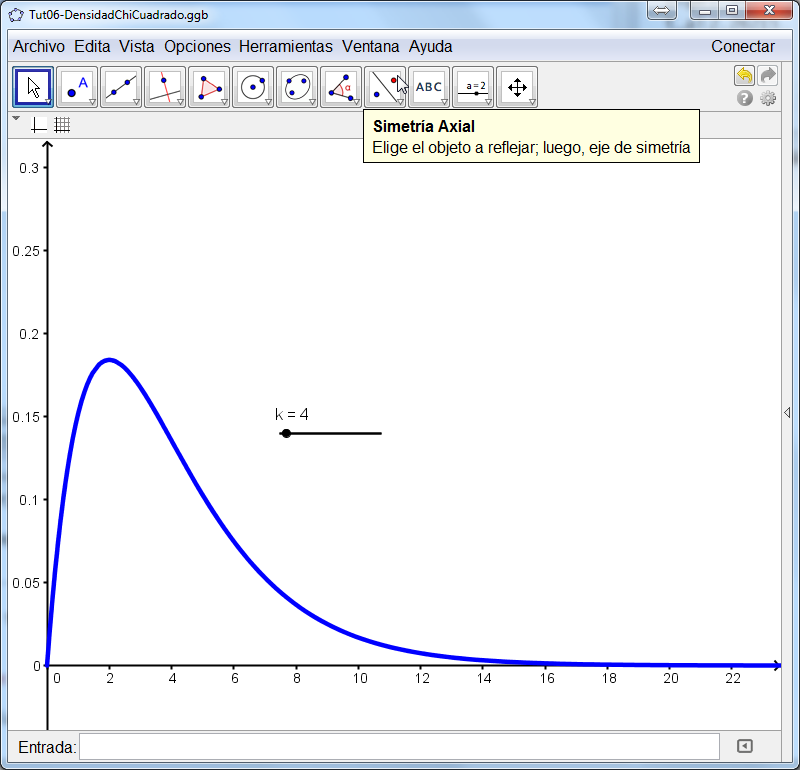
\includegraphics[width=9cm]{../fig/Tut06-36.png}
    \end{center}
Usa el deslizador para cambiar los valores de $k$ y explorar así esta familia de distribuciones. No dejes de observar el comportamiento cuando $k=1$, que es excepcional dentro de la familia. Además de esto, observa el aspecto y posición de la función de densidad cuando $k$ crece (tal vez tengas que hacer zoom para verlo). En particular comprobarás que la media de la distribución $\chi^2_k$ aumenta a medida que $k$ aumenta. Esta primera exploración debe servir para recordar dos aspectos básicos que {\bf nunca debemos olvidar} al trabajar con $\chi^2$:
\begin{itemize}
  \item La distribución sólo es distinta de cero en los valores positivos (una variable $\chi^2$ no toma valores negativos; al fin y al cabo, es un cuadrado).
  \item En consecuencia, la distribución {\bf no es simétrica} en ningún sentido.
\end{itemize}
Estas características de la distribución condicionan y complican ligeramente el trabajo que tenemos que hacer. La {\em Calculadora de Probabilidades} de GeoGebra es un buen punto de partida para empezar a trabajar con esta distribución. La siguiente figura muestra la situación que, por defecto, nos encontramos al abrir la {\em Calculadora} y seleccionar $\chi^2$ en el menú desplegable.

    \begin{center}
    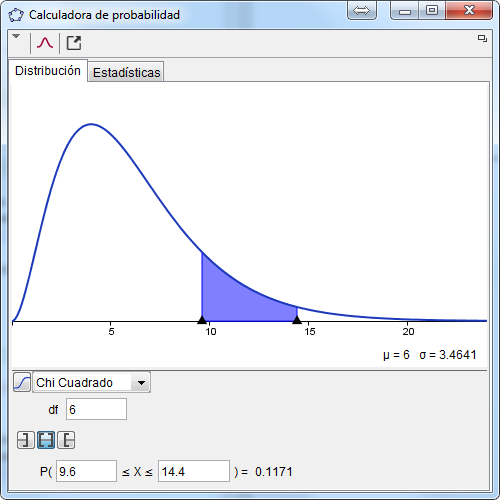
\includegraphics[width=10cm]{../fig/Tut06-29.png}
    \end{center}

La mejor manera de adentrarnos en este terreno es con una lista de problemas directos e inversos de probabilidad.

\begin{ejercicio}
\label{tut06:ejercicio17}
Sea $Y$ una variable aleatoria de tipo $\chi^2_9$ (con $k=9$ grados de libertad). Usa la Calculadora de Probabilidades de GeoGebra para calcular estos valores:
    \begin{enumerate}
        \item $P(Y\leq 2.09)$
        \item $P(Y\geq 11.4)$
        \item $P(14.7\leq Y\leq 16.9)$
        \item Valor de $y$ tal que $P(Y\geq y)=0.05$.
        \item Valor de $y$ tal que $P(Y\leq y)=0.01$.
        \item Valores $y_1, y_2$ tales que $P(y_1\leq Y\leq y_2)=0.90$ y además $P(Y\leq y_1)=P(Y\geq y_2)$.
    \end{enumerate}
Soluciones en la página \pageref{tut06:ejercicio17:sol}.
\qed
\end{ejercicio}

Aparte de la {\em Calculadora de Probabilidades}, en GeoGebra disponemos de la función {\tt ChiCuadrado} para efectuar cálculos de probabilidad, usando como en R la cola izquierda de la distribución. Por ejemplo, la respuesta del apartado 1 del Ejercicio \ref{tut06:ejercicio17} se puede obtener con:
\begin{verbatim}
    ChiCuadrado[9, 2.09]
\end{verbatim}
Recuerda que las soluciones se obtienen en la {\em Vista Algebraica} de GeoGebra. Como ves, los grados de libertad se colocan en el primer argumento de la función.  Para resolver problemas inversos dispones de la función {\tt ChiCuadradoInversa}. Con esa función el apartado 5 del Ejercicio \ref{tut06:ejercicio17} se resuelve así:
\begin{verbatim}
    ChiCuadradoInversa[9, 0.01]
\end{verbatim}

\begin{ejercicio}
\label{tut06:ejercicio18}
Usa estas funciones para comprobar las soluciones de los restantes apartados del Ejercicio \ref{tut06:ejercicio17}.
Soluciones en la página \pageref{tut06:ejercicio18:sol}.
\qed
\end{ejercicio}

\subsection{$\chi^2$ en R.}
\label{tut06:subsec:Chi2EnR}

En R disponemos, como era previsible, de cuatro funciones llamadas  {\tt dchisq}, {\tt rchisq}, {\tt pchisq} y {\tt qchisq}. El papel de cada una de estas cuatro funciones, a estas alturas, empieza a ser evidente a partir de sus nombres: {\tt dchisq} es es la función de densidad (y apenas vamos a usarla en este curso), {\tt pchisq} es la función de distribución (probabilidad de la cola izquierda), {\tt qchisq} proporciona los cuantiles (de nuevo, usando la cola izquierda) y, finalmente, {\tt rchisq} sirve para generar valores aleatorios de una variable de tipo $\chi^2_k$.  Los grados de libertad (el valor de $k$) se indican, en todas estas funciones, con el argumento {\tt df}, como sucedía en la $t$ de Student.

Como ejemplo, vamos a usar {\tt pchisq} para resolver un par de problemas directos de probabilidad asociados con $\chi^2_k$. Por ejemplo, para calcular la probabilidad de esta cola derecha
\[P(\chi^2_{14} > 7)\]
usamos uno de estos dos comandos indistintamente:
\begin{knitrout}
\definecolor{shadecolor}{rgb}{0.969, 0.969, 0.969}\color{fgcolor}\begin{kframe}
\begin{alltt}
\hlnum{1} \hlopt{-} \hlkwd{pchisq}\hlstd{(}\hlnum{7}\hlstd{,} \hlkwc{df}\hlstd{=}\hlnum{14}\hlstd{)}
\end{alltt}
\begin{verbatim}
## [1] 0.93471
\end{verbatim}
\begin{alltt}
\hlkwd{pchisq}\hlstd{(}\hlnum{7}\hlstd{,} \hlkwc{df}\hlstd{=}\hlnum{14}\hlstd{,} \hlkwc{lower.tail}\hlstd{=}\hlnum{FALSE}\hlstd{)}
\end{alltt}
\begin{verbatim}
## [1] 0.93471
\end{verbatim}
\end{kframe}
\end{knitrout}
mientras que para encontrar el valor $y$ tal que
\[P( \chi^2_3 > y ) = 0.1\]
usaríamos uno de estos comandos:
\begin{knitrout}
\definecolor{shadecolor}{rgb}{0.969, 0.969, 0.969}\color{fgcolor}\begin{kframe}
\begin{alltt}
\hlkwd{qchisq}\hlstd{(}\hlnum{1} \hlopt{-}\hlnum{0.1}\hlstd{,} \hlkwc{df}\hlstd{=}\hlnum{3}\hlstd{)}
\end{alltt}
\begin{verbatim}
## [1] 6.2514
\end{verbatim}
\begin{alltt}
\hlkwd{qchisq}\hlstd{(}\hlnum{0.1}\hlstd{,} \hlkwc{df}\hlstd{=}\hlnum{3}\hlstd{,} \hlkwc{lower.tail}\hlstd{=}\hlnum{FALSE}\hlstd{)}
\end{alltt}
\begin{verbatim}
## [1] 6.2514
\end{verbatim}
\end{kframe}
\end{knitrout}
Para que practiques el uso de estas funciones, haremos un ejercicio.
\begin{ejercicio}
\label{tut06:ejercicio19}
\begin{enumerate}
  \item[]
  \item Repite con R el Ejercicio \ref{tut06:ejercicio17}.
  \item Usa R para comprobar los resultados del Ejemplo \ref{curso-cap06:ejem:ProblemaDirectoInversoProbabilidadChi} del libro (pág. \pageref{curso-cap06:ejem:ProblemaDirectoInversoProbabilidadChi})
\end{enumerate}

Soluciones en la página \pageref{tut06:ejercicio19:sol}.
\qed
\end{ejercicio}

\subsection{$\chi^2$ en Wolfram Alpha.}
\label{tut06:subsec:Chi2EnWolframAlpha}

El trabajo con $\chi^2_k$ en Wolfram Alpha es muy parecido al que hicimos con la $t$ de Student. Por ejemplo,  este problema directo de probabilidad
\[P(10 < \chi^2_{12} < 15)\]
se resuelve con este comando:
\begin{verbatim}
    P[10 < Y < 15] for Y chi-square with 12 dof
\end{verbatim}
Y el resultado aproximado es $0.3745$. Los problemas directos son muy fáciles de resolver, pero los inversos nos darán algo más de trabajo. Para encontrar, por ejemplo, el valor $y$ tal que
\[P( \chi^2_{7} > y) = \dfrac{7}{13}\]
tenemos que comprender primero que esto es lo mismo que buscar el valor de $y$ tal que
\[P( \chi^2_{7} \leq y) = 1 - \dfrac{7}{13} = \dfrac{6}{13}\approx 0.46154,\]
y ahora usar este comando en Wolfram Alpha:
\begin{center}
    46.154th percentile  for chi-square with 7 dof
\end{center}
El resultado aproximado es $6.01105$.

\begin{ejercicio}
\label{tut06:ejercicio20}
Comprueba estos dos ejemplos con R y GeoGebra. Soluciones en la página \pageref{tut06:ejercicio20:sol}.
\qed
\end{ejercicio}

\section{Intervalos de confianza para la varianza con $\chi^2$.}
\label{tut06:sec:IntervalosConfianzaVarianzaChiCuadrado}

A la hora de construir un intervalo de confianza la asimetría de la distribución $\chi^2_k$ marca una diferencia importante con las otras distribuciones que hemos visto antes. En el trabajo con la $Z$ y la $t$ de Student, podíamos aprovechar la simetría para calcular un único valor crítico, con la seguridad de que si, por ejemplo, $z_{\alpha/2}$ deja una probabilidad igual a $\alpha/2$ a su derecha, entonces el simétrico $-z_{\alpha/2}$ deja una probabilidad $\alpha/2$ a su izquierda. Con $\chi^2$ esto no es así, y tendremos que calcular dos valores críticos, $\chi^2_{k;\alpha/2}$, pero también $\chi^2_{k;1-\alpha/2}$. Esos son los valores necesarios para construir el intervalo de confianza para $\sigma^2$  (en poblaciones normales) que hemos visto en la Ecuación \ref{curso-cap06:ecu:IntervaloConfianzaDesviacionTipica} (pág. \pageref{curso-cap06:ecu:IntervaloConfianzaDesviacionTipica}) del libro:
       \[
       \sqrt{\dfrac{(n-1)s^2}{\chi^2_{k,\alpha/2}}}\leq\sigma\leq\sqrt{\dfrac{(n-1)s^2}{\chi^2_{k,1-\alpha/2}}}.
       \]

Vamos a ver como construir estos intervalos en varios de los programas que venimos utilizando.

\subsection{Intervalo de confianza para $\sigma$ con R.}
\label{tut06:subsec:IntConfSIgmaConR}

Para fijar ideas, supongamos que tenemos una muestra, procedente de una población normal, de tamaño $n=18$ (de manera que los grados de libertad son $k=n-1=17$), en la que  $s= 2.1$, y queremos construir un intervalo de confianza para $\sigma$ a un nivel de confianza del $99\%$.  Para seguir la discusión es bueno que tengas presente la Figura \ref{curso-cap06:fig:ChiCuadradoValoresCriticosIntervalo} del libro (pág. \pageref{curso-cap06:fig:ChiCuadradoValoresCriticosIntervalo}), que reproducimos aquí por comodidad. ¡Pero atención! Esa figura se corresponde a otro valor de $k$, así que no esperes que los valores críticos estén donde indica la figura.

\begin{center}
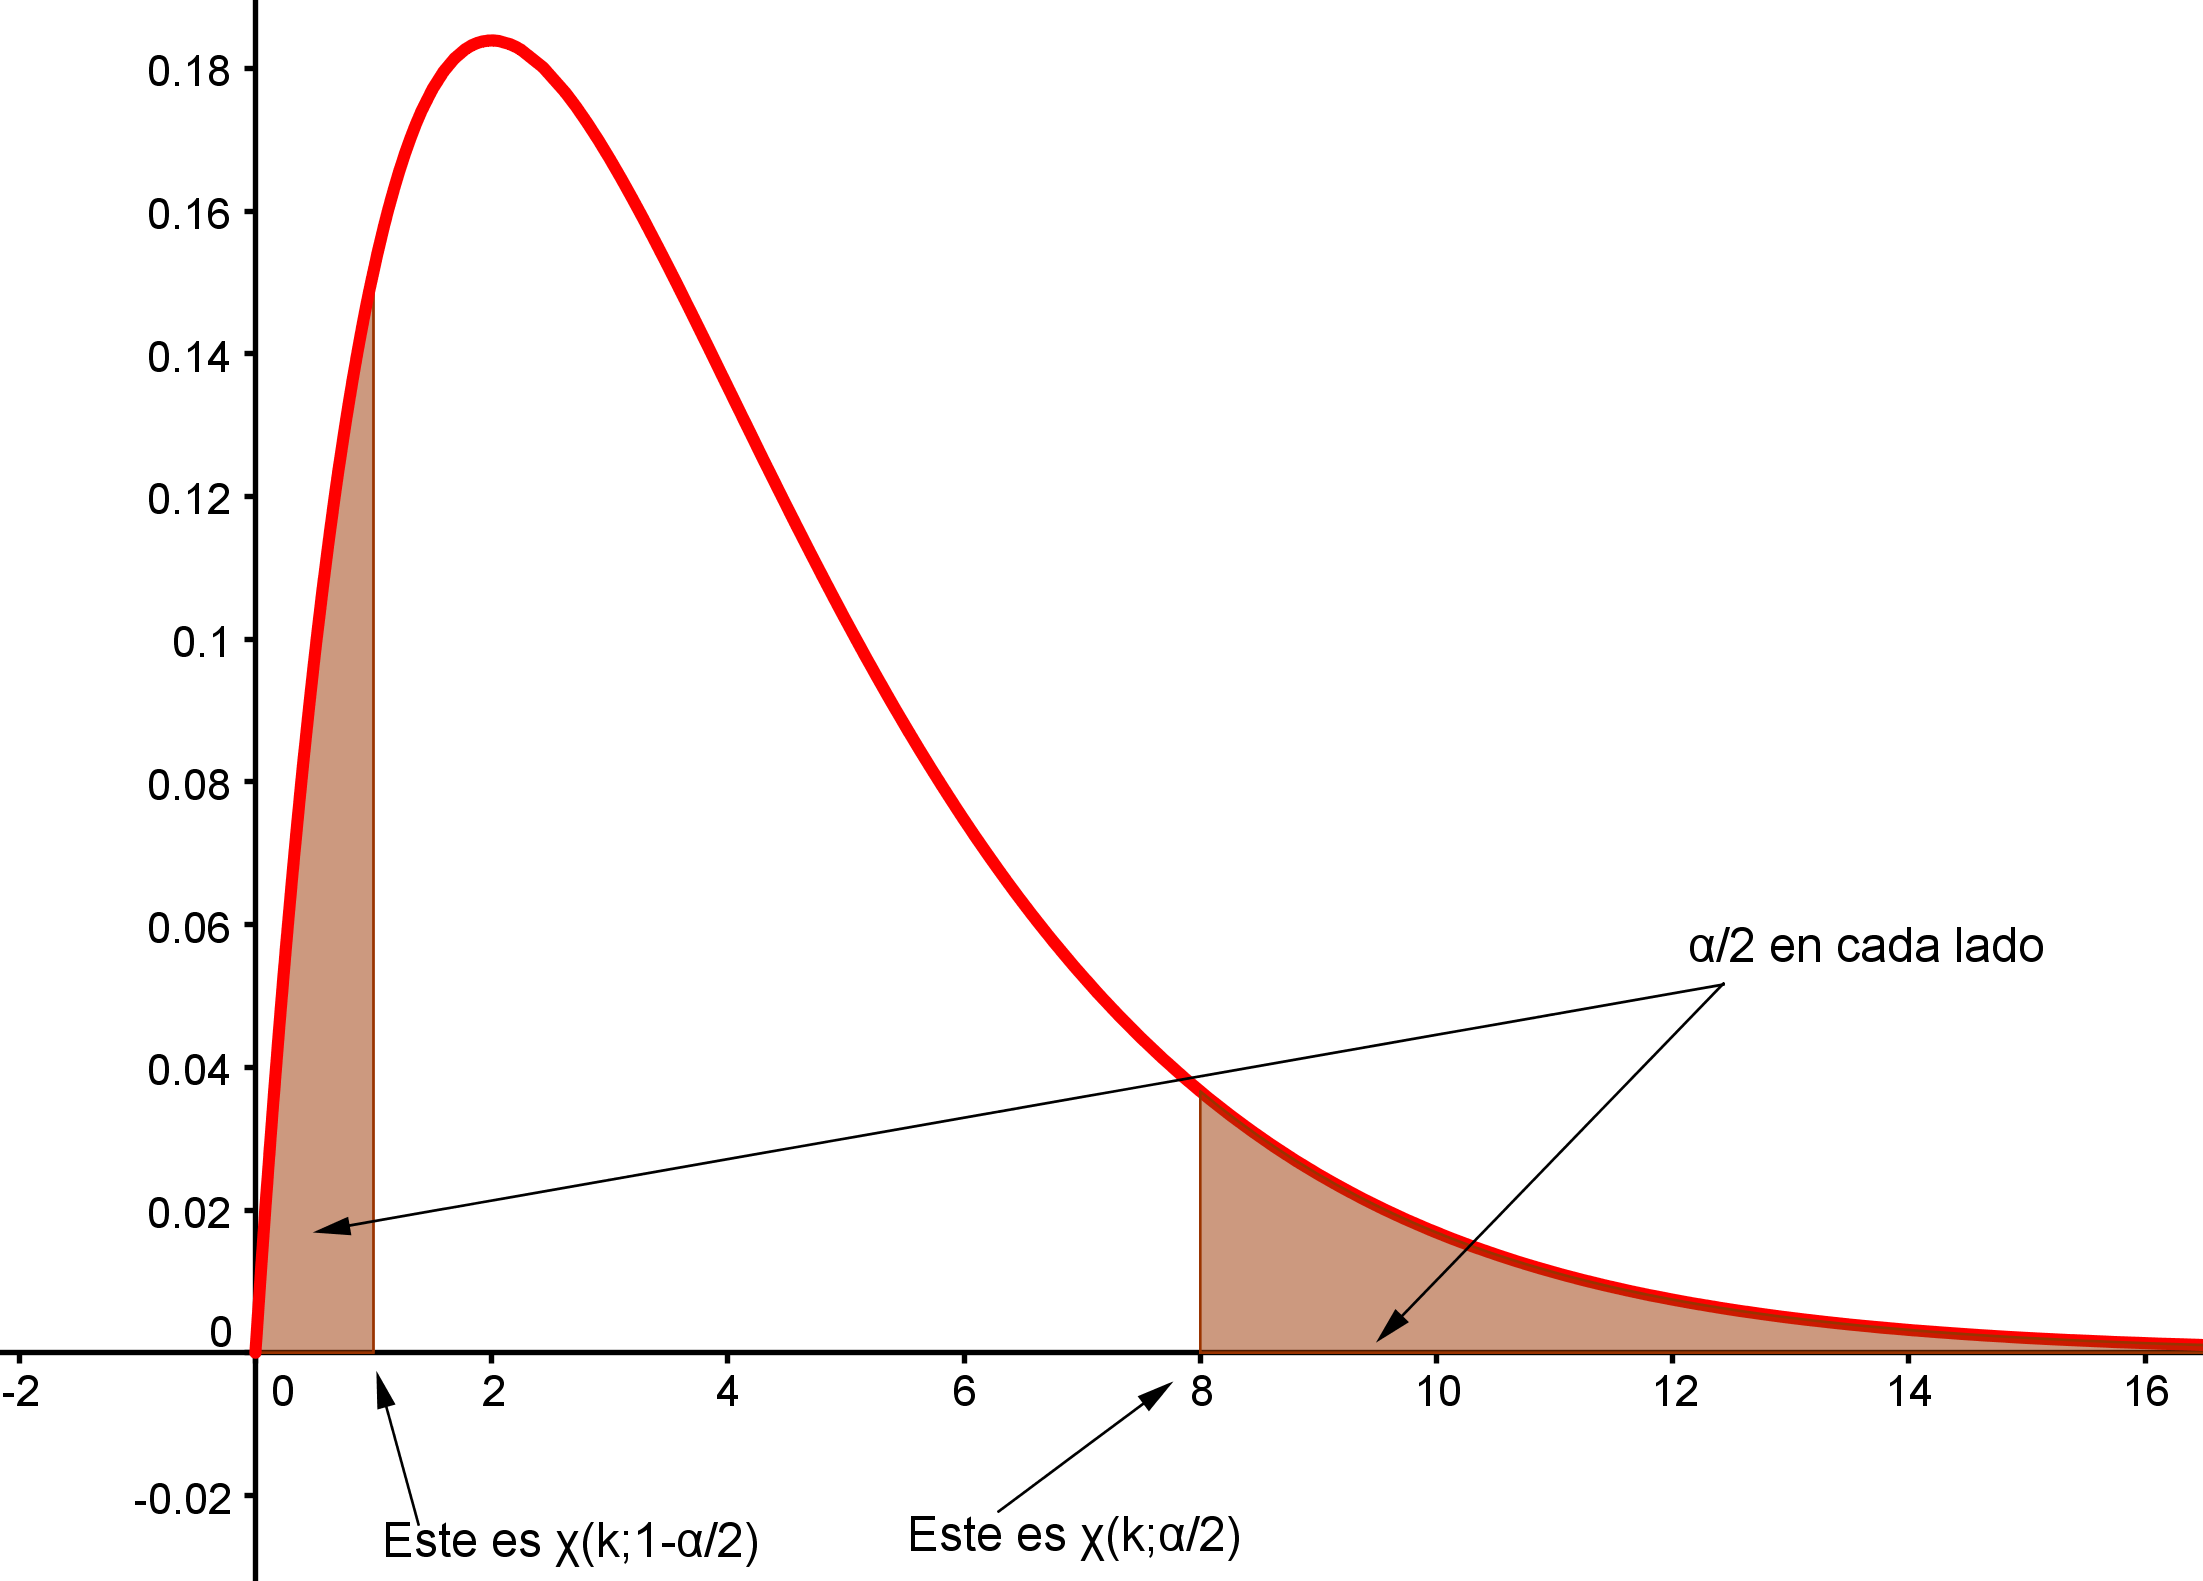
\includegraphics[width=13cm]{../fig/Cap06-ChiCuadradoValoresCriticosIntervalo.png}
\end{center}

Por lo tanto, para comenzar la búsqueda de los valores críticos hacemos en R:
\begin{knitrout}
\definecolor{shadecolor}{rgb}{0.969, 0.969, 0.969}\color{fgcolor}\begin{kframe}
\begin{alltt}
\hlstd{n} \hlkwb{=} \hlnum{17}
\hlstd{k} \hlkwb{=} \hlstd{n} \hlopt{-} \hlnum{1}
\hlstd{s} \hlkwb{=} \hlnum{2.1}

\hlstd{nc} \hlkwb{=} \hlnum{0.99}
\hlstd{(alfa} \hlkwb{=} \hlnum{1} \hlopt{-} \hlstd{nc)}
\end{alltt}
\begin{verbatim}
## [1] 0.01
\end{verbatim}
\begin{alltt}
\hlstd{(alfa2} \hlkwb{=} \hlstd{alfa} \hlopt{/}\hlnum{2}\hlstd{)}
\end{alltt}
\begin{verbatim}
## [1] 0.005
\end{verbatim}
\end{kframe}
\end{knitrout}
Para  construir el intervalo necesitamos calcular el valor crítico situado más a la derecha, que deja una probabilidad $\frac{\alpha}{2}=0.005$ en su cola derecha (y $\alpha/2 = 0.995$ en la cola izquierda que usa R), al que hemos llamado:
\[\chi^2_{k;\alpha/2} = \chi^2_{16;0.005}\]
Este valor crítico se obtiene en R con:
\begin{knitrout}
\definecolor{shadecolor}{rgb}{0.969, 0.969, 0.969}\color{fgcolor}\begin{kframe}
\begin{alltt}
\hlstd{(chiAlfa2} \hlkwb{=} \hlkwd{qchisq}\hlstd{(}\hlnum{1} \hlopt{-} \hlstd{alfa2,} \hlkwc{df}\hlstd{=k))}
\end{alltt}
\begin{verbatim}
## [1] 34.267
\end{verbatim}
\end{kframe}
\end{knitrout}
También necesitamos el otro valor crítico situado más a la izquierda, el que deja una probabilidad $\frac{\alpha}{2}=0.005$ en su cola izquierda:
\[\chi^2_{k;1 - \alpha/2} = \chi^2_{k;0.995}\]
que en R se obtiene con:
\begin{knitrout}
\definecolor{shadecolor}{rgb}{0.969, 0.969, 0.969}\color{fgcolor}\begin{kframe}
\begin{alltt}
\hlstd{(chiUnoMenosAlfa2} \hlkwb{=} \hlkwd{qchisq}\hlstd{(alfa2,} \hlkwc{df}\hlstd{=k))}
\end{alltt}
\begin{verbatim}
## [1] 5.1422
\end{verbatim}
\end{kframe}
\end{knitrout}
Lee varias veces esto si te pierdes. Sabemos que la notación $\chi^2_{k;p}$ es un poco complicada, porque $p$ se refiere a la probabilidad en la cola derecha, y R usa la cola izquierda. Pero es mejor que lo pienses detenidamente, para evitar que este pequeño embrollo notacional te juegue una mala pasada.


Una vez construidos los dos valores críticos, el intervalo es muy fácil de construir. Sólo una última advertencia: el valor crítico situado a la {\em derecha} se usa en realidad para calcular el extremo {\em izquierdo} del intervalo, y viceversa. En cualquier caso, si alguna vez te equivocas, los extremos del intervalo se intercambiarían, y eso te serviría de advertencia de que debes revisar tus cuentas para comprobar que no se debe a ningún otro error.

La construcción del intervalo se realiza mediante una operación vectorial de R, en la que obtenemos a la vez los dos extremos:
\begin{knitrout}
\definecolor{shadecolor}{rgb}{0.969, 0.969, 0.969}\color{fgcolor}\begin{kframe}
\begin{alltt}
\hlstd{(intervalo} \hlkwb{=} \hlstd{s} \hlopt{*} \hlkwd{sqrt}\hlstd{(k} \hlopt{/} \hlkwd{c}\hlstd{(chiAlfa2, chiUnoMenosAlfa2)))}
\end{alltt}
\begin{verbatim}
## [1] 1.4350 3.7043
\end{verbatim}
\end{kframe}
\end{knitrout}
Así que el intervalo de confianza para $\sigma$ al $99\%$ es:
\[1.435 < \sigma < 3.704.\]
Si lo que deseamos es un intervalo de confianza para la varianza $\sigma^2$ basta con elevar al cuadrado la desigualdad:
\[2.059 < \sigma^2 < 13.72.\]

\begin{ejercicio}
\label{tut06:ejercicio21}
Usa R para comprobar los resultados del Ejemplo \ref{curso-cap06:ejem:IntervaloConfianzaVarianzaLatasConserva}  del libro (pág. \pageref{curso-cap06:ejem:IntervaloConfianzaVarianzaLatasConserva})
Solución en la página \pageref{tut06:ejercicio21:sol}.
\qed
\end{ejercicio}



\subsubsection*{Ficheros ``plantilla'' de R para intervalos de confianza para $\sigma$.}

Hemos hecho el cálculo anterior paso a paso para que puedas entender cómo se calculan estos intervalos de confianza en R. Pero, como sucede siempre, una vez que se ha entendido esto, lo mejor es tratar de automatizar el proceso de construcción de los intervalos, y para conseguirlo incluimos dos ficheros ``plantilla'' de código R, que apenas necesitan presentación. El primero de ellos es para {\em problemas de libro de texto}, y el segundo para trabajar a partir de {\em datos en bruto}.
\begin{center}
\begin{tabular}{l}
\fichero{./code/Tut06-IntConf-DesvTipica-PoblNormal-Estadisticos.R}{Tut06-IntConf-DesvTipica-PoblNormal-Estadisticos.R}\\[3mm]
\fichero{./code/Tut06-IntConf-DesvTipica-PoblNormal-MuestraEnBruto.R}{Tut06-IntConf-DesvTipica-PoblNormal-MuestraEnBruto.R}
\end{tabular}
\end{center}
Abre los dos ficheros y estudia su código. Verás, entre otras cosas, que se obtienen dos intervalos, uno para $\sigma^2$ y  otro para $\sigma$. Vamos a practicar el uso de estos ficheros con algunos ejercicios.

\begin{ejercicio}
\label{tut06:ejercicio22}
\begin{enumerate}
  \item[]

  \item Usa estos ficheros para repetir la construcción del intervalo que hemos usado como ejemplo al principio de la Sección \ref{tut06:subsec:IntConfSIgmaConR}.

  \item Una muestra de tamaño $n=87$ de una población normal tiene una cuasidesviación típica igual a $s=2.81$. Calcula intervalos de confianza al $95\%$ para la varianza y desviación típica de esa población.

  \item El fichero adjunto
      \begin{center}
      \fichero{../datos/Tut06-datosIntConfDesvTipica.csv}{Tut06-datosIntConfDesvTipica.csv}
      \end{center}
      contiene una muestra con datos procedentes de una distribución normal. Calcula intervalos de confianza al $95\%$ para la varianza y desviación típica de esa población.
\end{enumerate}
Soluciones en la página \pageref{tut06:ejercicio22:sol}.
\qed
\end{ejercicio}

\subsection{Intervalo de confianza para $\sigma$ con GeoGebra y Wolfram Alpha.}
\label{tut06:subsec:IntConfSIgmaConGgbWolframAlpha}

\subsubsection{Wolfram Alpha.}

Para calcular intervalos de tipo {\em libro de texto} en Wolfram Alpha, puedes teclear esto en la línea de entrada del programa:
\begin{verbatim}
    confidence interval for the standard deviation of a normal population
\end{verbatim}
Al hacerlo, aparecerá un cuadro de diálogo en el que puedes introducir los valores necesarios para el cálculo del intervalo. En la siguiente figura se ilustra el cálculo del intervalo de confianza que hemos usado como primer ejemplo para R:
    \begin{center}
    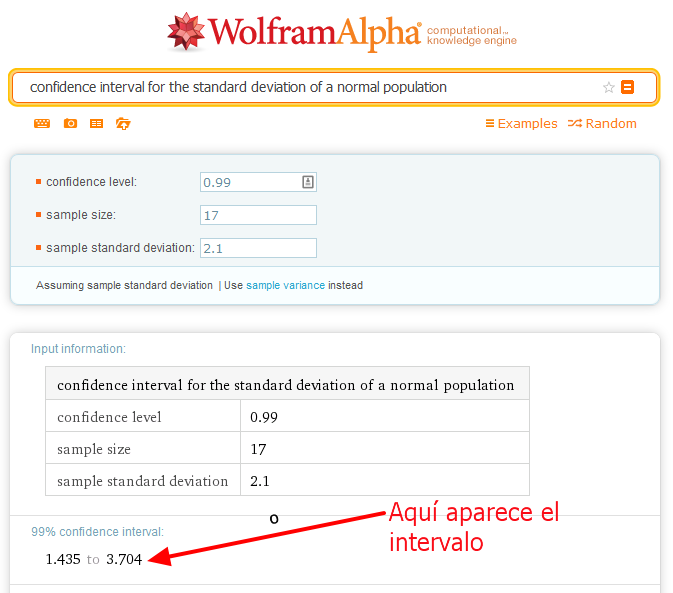
\includegraphics[width=13cm]{../fig/Tut06-37.png}
    \end{center}
Si lo que tienes es la muestra en bruto, tendrás que calcular los valores necesarios ($n$ y $s$, en realidad) por algún otro procedimiento, antes de poder usar Wolfram Alpha.

\subsubsection{GeoGebra.}

GeoGebra no ofrece, en su versión actual (la 4.4 en el momento de escribir esto) ninguna función específica para calcular estos intervalos. Naturalmente, dado que podemos calcular los cuantiles de $\chi^2_k$, siempre es posible hacer la construcción paso a paso, como hicimos al empezar la discusión con R.

\begin{ejercicio}
\label{tut06:ejercicio23}
Repite esa construcción paso a paso usando GeoGebra. Es decir, suponiendo que hemos tomado una muestra procedente de una población normal, de tamaño $n=18$ y en la que  $s= 2.1$, usa las funciones de GeoGebra para construir un intervalo de confianza para $\sigma$ a un nivel de confianza del $99\%$. Solución en la página \pageref{tut06:ejercicio23:sol}.
\qed
\end{ejercicio}

\section{Las funciones de la librería {\tt asbio} de R.}
\label{tut06:sec:LibreriaAsbio}

En la Sección \ref{tut06:subsec:IntConfMediaUsandoTConTtest} (pág. \pageref{tut06:subsec:IntConfMediaUsandoTConTtest}) hemos visto que la función {\tt t.test} de R se puede usar para obtener intervalos de confianza en el caso de muestras pequeñas. Pero, a diferencia de lo que sucede con la $t$ de Student, R no incluye, en la instalación básica,  funciones que permitan calcular intervalos de confianza para la media usando $Z$, o para $\sigma^2$ usando $\chi^2$. Hay, sin embargo,  varias librerías que ofrecen ese tipo de fórmulas. Nosotros vamos a utilizar una, bastante completa, llamada {\tt asbio}, creada por Ken Aho. Puedes encontrar información sobre esta librería en el enlace:
\begin{center}
\link{http://cran.r-project.org/web/packages/asbio/index.html}{http://cran.r-project.org/web/packages/asbio/index.html}
\end{center}
en el que encontrarás, entre otras cosas el manual en formato pdf.

Recuerda que antes de usar la librería {\tt asbio} debes instalarla (en la Sección \ref{tut03-tut03:sec:SolucionesEjerciciosAdicionales} del Tutorial03 se explica como instalar librerías adicionales en R). Después de instalarla, para usarla debes cargarla en la memoria del ordenador  utilizando el comando:
\begin{knitrout}
\definecolor{shadecolor}{rgb}{0.969, 0.969, 0.969}\color{fgcolor}\begin{kframe}
\begin{alltt}
    \hlkwd{library}\hlstd{(asbio)}
\end{alltt}


{\ttfamily\noindent\itshape\color{messagecolor}{\#\# Loading required package: tcltk}}\end{kframe}
\end{knitrout}
La librería {\tt asbio} incluye muchas funciones, pero las tres que más nos interesan en este momento son
{\tt ci.mu.z},   {\tt ci.mu.t} y {\tt  ci.sigma}. Todas ellas permiten calcular intervalos de confianza ({\tt ci} proviene del inglés {\em confidence interval}). Concretamente:
\begin{itemize}
  \item {\tt ci.mu.z} calcula intervalos de confianza  para la media usando $Z$.
  \item {\tt ci.mu.t} calcula intervalos de confianza  para la media usando $t$ de Student. Es decir, lo mismo que antes hemos visto con {\tt t.test}.
  \item {\tt ci.sigma} calcula intervalos de confianza {\bf para la varianza} $\sigma^2$  (¡y no para $\sigma$, a pesar del nombre!) usando $\chi^2$.
\end{itemize}
Y en todos los casos podemos partir de un vector (datos {\em en bruto}), o de los estadísticos que resumen la muestra (los que hemos llamado {\em problemas de libro de texto}). Para distinguir en qué caso estamos, basta con utilizar el argumento booleano {\tt summarized}: si es {\tt summarized=TRUE} usamos los valores resumidos ($n$, $\bar X$, $s$ o $\sigma$), mientras que si es {\tt summarized=FALSE}, usamos la muestra {\em en bruto}.

Vamos a ver como usar estas funciones mediante algunos ejemplos, basados en ejercicios que hemos propuesto anteriormente en este tutorial.

\subsubsection*{Ejemplos con {\tt ci.mu.z}}

En el apartado 3 del Ejercicio \ref{tut06:ejercicio06} (pág. \pageref{tut06:ejercicio06}) teníamos una muestra de 450 elementos de una población normal, con cuasidesviación típica $s=2.3$, y una media muestral $\bar X=132.5$. Para calcular un intervalo de confianza al 99\% para la media $\mu$, teniendo en cuenta el tamaño de la muestra podemos usar la distribución normal $Z$.  Podemos por tanto utilizar la función {\tt ci.mu.z}, con la opción {\tt summarized=TRUE}, de esta manera:
\begin{knitrout}
\definecolor{shadecolor}{rgb}{0.969, 0.969, 0.969}\color{fgcolor}\begin{kframe}
\begin{alltt}
\hlstd{(intAsBio} \hlkwb{=} \hlkwd{ci.mu.z}\hlstd{(}\hlkwc{n}\hlstd{=}\hlnum{450}\hlstd{,} \hlkwc{sigma}\hlstd{=}\hlnum{2.3}\hlstd{,} \hlkwc{xbar}\hlstd{=}\hlnum{132.5}\hlstd{,} \hlkwc{conf}\hlstd{=}\hlnum{0.99}\hlstd{,} \hlkwc{summarized}\hlstd{=}\hlnum{TRUE}\hlstd{))}
\end{alltt}
\begin{verbatim}
## 
## 99% z Confidence interval for population mean 
## Estimate     0.5%    99.5% 
##   132.50   132.22   132.78
\end{verbatim}
\end{kframe}
\end{knitrout}
Compara esto con lo que obtuvimos en el Ejercicio \ref{tut06:ejercicio06}. La respuesta de la función {\tt ci.mu.z} es, en realidad, una {\em lista} de R (puedes usar {\tt class} para comprobarlo). Ya nos hemos encontrado antes con este tipo de situaciones, en las que para acceder a los resultados tenemos que utilizar el operador \verb/$/. Para saber cuales son los elementos de una lista (o de cualquier otro objero de R), disponemos de la función {\tt str}, que en este caso produce:
\begin{knitrout}
\definecolor{shadecolor}{rgb}{0.969, 0.969, 0.969}\color{fgcolor}\begin{kframe}
\begin{alltt}
\hlkwd{str}\hlstd{(intAsBio)}
\end{alltt}
\begin{verbatim}
## List of 4
##  $ margin: num 0.279
##  $ ci    : num [1:3] 132 132 133
##  $ head  : chr "99% z Confidence interval for population mean"
##  $ ends  : chr [1:3] "Estimate" "0.5%" "99.5%"
##  - attr(*, "class")= chr "ci"
\end{verbatim}
\end{kframe}
\end{knitrout}
Nos interesa el elemento {\tt ci} de esta lista. Y podemos acceder a ese elemento con este comando
\begin{knitrout}
\definecolor{shadecolor}{rgb}{0.969, 0.969, 0.969}\color{fgcolor}\begin{kframe}
\begin{alltt}
\hlstd{intAsBio}\hlopt{$}\hlstd{ci}
\end{alltt}
\begin{verbatim}
## [1] 132.50 132.22 132.78
\end{verbatim}
\end{kframe}
\end{knitrout}
Así se obtiene un vector con tres componentes. La primera es $\bar X$, y las dos últimas son los extremos del intervalo de confianza. Podemos usarlos, por tanto

para, por ejemplo, calcular la semianchura del intervalo, de esta manera:
\begin{knitrout}
\definecolor{shadecolor}{rgb}{0.969, 0.969, 0.969}\color{fgcolor}\begin{kframe}
\begin{alltt}
\hlstd{(semianchura} \hlkwb{=} \hlstd{(intAsBio}\hlopt{$}\hlstd{ci[}\hlnum{3}\hlstd{]} \hlopt{-} \hlstd{intAsBio}\hlopt{$}\hlstd{ci[}\hlnum{2}\hlstd{])} \hlopt{/} \hlnum{2}\hlstd{)}
\end{alltt}
\begin{verbatim}
## [1] 0.27928
\end{verbatim}
\end{kframe}
\end{knitrout}
Ahora puedes comprobar que la semianchura es el elemento {\tt margin} de la lista {\tt intAsBio} que hemos obtenido como salida de {\tt ci.mu.z}:
\begin{knitrout}
\definecolor{shadecolor}{rgb}{0.969, 0.969, 0.969}\color{fgcolor}\begin{kframe}
\begin{alltt}
\hlstd{intAsBio}\hlopt{$}\hlstd{margin}
\end{alltt}
\begin{verbatim}
## [1] 0.27928
\end{verbatim}
\end{kframe}
\end{knitrout}
El resto de los elementos de {\tt intAsBio} son simplemente rótulos.

Vamos ahora a usar a calcular un intervalo de confianza a partir de datos {\em en bruto}, usando el fichero {\tt Tut06-IntConf-Media-UsandoZ-datos.csv} del apartado 5 del Ejercicio \ref{tut06:ejercicio06}. Esto nos va a servir para descubrir una peculiaridad {\bf muy importante} de esta función. Para ello nos aseguramos de que el fichero {\tt csv} está en el directorio de trabajo de R, y usamos de nuevo {\tt ci.mu.z}, pero ahora con {\tt summarized=FALSE}:
\begin{knitrout}
\definecolor{shadecolor}{rgb}{0.969, 0.969, 0.969}\color{fgcolor}\begin{kframe}
\begin{alltt}
\hlstd{muestra} \hlkwb{=} \hlkwd{read.table}\hlstd{(}\hlkwc{file}\hlstd{=}\hlstr{"../datos/Tut06-IntConf-Media-UsandoZ-datos.csv"}\hlstd{,} \hlkwc{sep}\hlstd{=}\hlstr{" "}\hlstd{,} \hlkwc{dec}\hlstd{=}\hlstr{"."}\hlstd{)[ ,}\hlnum{1}\hlstd{]}
\hlstd{(intAsBio} \hlkwb{=} \hlkwd{ci.mu.z}\hlstd{(}\hlkwc{data}\hlstd{=muestra,} \hlkwc{conf}\hlstd{=}\hlnum{0.95}\hlstd{,} \hlkwc{summarized}\hlstd{=}\hlnum{FALSE}\hlstd{,} \hlkwc{sigma} \hlstd{=} \hlkwd{sd}\hlstd{(muestra)))}
\end{alltt}
\begin{verbatim}
## 
## 95% z Confidence interval for population mean 
## Estimate     2.5%    97.5% 
##   7.2313   7.0932   7.3694
\end{verbatim}
\end{kframe}
\end{knitrout}
Como ves, en el caso de datos {\em en bruto} hemos tenido que pedirle explícitamente a {\tt ci.mu.z} que use la cuasidesviación típica de la muestra, calculada con {\tt sd}. Si no haces esto, comprobarás que el resultado no es correcto.
\begin{ejercicio}
\label{tut06:ejercicio24}
Compruébalo. Solución en la página \pageref{tut06:ejercicio24:sol}.
\qed
\end{ejercicio}

\subsubsection*{Ejemplos con {\tt ci.mu.t}}

Vamos a usar la función {\tt ci.mu.t} para hacer el apartado 2 del Ejercicio \ref{tut06:ejercicio06}. Tenemos una muestra de $10$ elementos de una población normal, con media muestral $\bar X=132.5$ y cuasidesviación típica $s=2.3$. Dado que la muestra es pequeña y desconocemos $\sigma$ debemos usar la $t$ de Student para calcular un intervalo  de confianza al 95\% para la media $\mu$. Lo hacemos así:
\begin{knitrout}
\definecolor{shadecolor}{rgb}{0.969, 0.969, 0.969}\color{fgcolor}\begin{kframe}
\begin{alltt}
\hlkwd{ci.mu.t}\hlstd{(}\hlkwc{n}\hlstd{=}\hlnum{10}\hlstd{,} \hlkwc{xbar}\hlstd{=}\hlnum{132.5}\hlstd{,} \hlkwc{sd}\hlstd{=}\hlnum{2.3}\hlstd{,} \hlkwc{conf}\hlstd{=}\hlnum{0.95}\hlstd{,} \hlkwc{summarized}\hlstd{=}\hlnum{TRUE}\hlstd{)}
\end{alltt}
\begin{verbatim}
## 
## 95% t Confidence interval for population mean 
## Estimate     2.5%    97.5% 
##   132.50   130.85   134.15
\end{verbatim}
\end{kframe}
\end{knitrout}
Puedes comprobar que el resultado coincide con lo que obtuvimos en la solución del Ejercicio \ref{tut06:ejercicio14} (pág. \pageref{tut06:ejercicio14:sol}) usando {\tt t.test}.\\

Si partes de una muestra {\em en bruto}, como la muestra
    \begin{verbatim}
    3.14, 3.71, 2.77, 4.08, 4.18, 1.51, 3.65, 3.41, 4.51, 2.27, 3.28,
    2.26, 2.80, 2.54, 3.77
    \end{verbatim}
del apartado 2 del Ejercicio \ref{tut06:ejercicio14}, entonces para calcular un intervalo de confianza al $95\%$ para $\mu$ haremos:
\begin{knitrout}
\definecolor{shadecolor}{rgb}{0.969, 0.969, 0.969}\color{fgcolor}\begin{kframe}
\begin{alltt}
\hlstd{muestra} \hlkwb{=} \hlkwd{c}\hlstd{(}\hlnum{3.14}\hlstd{,} \hlnum{3.71}\hlstd{,} \hlnum{2.77}\hlstd{,} \hlnum{4.08}\hlstd{,} \hlnum{4.18}\hlstd{,} \hlnum{1.51}\hlstd{,} \hlnum{3.65}\hlstd{,} \hlnum{3.41}\hlstd{,} \hlnum{4.51}\hlstd{,} \hlnum{2.27}\hlstd{,} \hlnum{3.28}\hlstd{,}
    \hlnum{2.26}\hlstd{,} \hlnum{2.80}\hlstd{,} \hlnum{2.54}\hlstd{,} \hlnum{3.77}\hlstd{)}
\hlstd{(intAsBio} \hlkwb{=} \hlkwd{ci.mu.t}\hlstd{(}\hlkwc{data}\hlstd{=muestra,} \hlkwc{conf}\hlstd{=}\hlnum{0.95}\hlstd{,} \hlkwc{summarized}\hlstd{=}\hlnum{FALSE}\hlstd{))}
\end{alltt}
\begin{verbatim}
## 
## 95% t Confidence interval for population mean 
## Estimate     2.5%    97.5% 
##   3.1920   2.7316   3.6524
\end{verbatim}
\end{kframe}
\end{knitrout}
Fíjate en que, en este caso, no ha sido necesario usar la opción {\tt sigma = sd(muestra)} para obtener el resultado correcto, a diferencia de lo que sucede con {\tt ci.mu.z}. Además, si la incluyes, desafortunadamente la función devuelve el error {\tt unused argument}.

\subsubsection*{Ejemplos con {\tt ci.mu.sigma}}

Vamos a empezar usando la función {\tt ci.mu.sigma} para repetir el apartado 2 del Ejercicio \ref{tut06:ejercicio22} (pág. \pageref{tut06:ejercicio22} y solución en la página \pageref{tut06:ejercicio22:sol}). En ese ejercicio teníamos una muestra de tamaño $n=87$ de una población normal, con cuasidesviación típica igual a $s=2.81$ y queríamos calcular un intervalo de confianza al $95\%$ para la varianza de esa población. Lo podemos hacer así:
\begin{knitrout}
\definecolor{shadecolor}{rgb}{0.969, 0.969, 0.969}\color{fgcolor}\begin{kframe}
\begin{alltt}
\hlkwd{ci.sigma}\hlstd{(}\hlkwc{n}\hlstd{=}\hlnum{87}\hlstd{,} \hlkwc{S.sq} \hlstd{=} \hlnum{2.81}\hlopt{^}\hlnum{2}\hlstd{,} \hlkwc{conf}\hlstd{=}\hlnum{0.95}\hlstd{,} \hlkwc{summarized}\hlstd{=}\hlnum{TRUE}\hlstd{)}
\end{alltt}
\begin{verbatim}
## 
## 95% Confidence interval for population variance 
## Estimate     2.5%    97.5% 
##   7.8961   5.9807  10.9107
\end{verbatim}
\end{kframe}
\end{knitrout}
{\bf Atención:} El argumento {\tt S.sq} es la cuasivarianza, no la cuasidesviación típica. Por eso hemos tenido que elevar {\tt 2.81} al cuadrado. Y el intervalo que se obtiene es para $\sigma^2$, no para $\sigma$ (a pesar del nombre de la función).

\begin{ejercicio}
\label{tut06:ejercicio25}
Usa {\tt ci.sigma} para calcular el intervalo de confianza a partir de una muestra {\em en bruto} (fichero {\tt csv}) que aparece en el apartado 3 del Ejercicio \ref{tut06:ejercicio22} (pág. \pageref{tut06:ejercicio22}). Solución en la página \pageref{tut06:ejercicio25:sol}.
\qed
\end{ejercicio}

Con esto hemos concluido nuestra primera visita a la librería {\tt asbio}. Volveremos sobre ella más adelante, en futuros tutoriales, y aprenderemos a usar otras funciones de esta librería.

%\textcolor{red}{\LARGE ESTOY AQUI.}

%
%
%\hrule
%\hrule
%\pendiente{Intervalos de predicción}
%

\section{Ejercicios adicionales y soluciones.}
\label{tut06:sec:EjerciciosAdicionalesYSoluciones}

\subsection*{Ejercicios adicionales.}
\label{tut06:subsec:EjerciciosAdicionales}

\begin{ejercicio}
\label{tut06:ejercicio26}


{\bf Simulaciones sobre  la interpretación probabilista de los intervalos de confianza.}\\
\noindent
En este ejercicio vamos a usar R para volver sobre la interpretación probabilística de los intervalos de confianza que vimos, usando GeoGebra, en la Sección \ref{tut06:subsubsec:InterpretacionProbabilisticaIntConfGeoGebra} de este tutorial (pág. \pageref{tut06:subsubsec:InterpretacionProbabilisticaIntConfGeoGebra}). Para hacerlo vamos a construir algunas simulaciones.

\begin{enumerate}
  \item Empieza por usar {\tt rnorm} para generar un número grande (por ejemplo $N=1000$) de muestras de una población norma, cada una de tamaño por ejemplo $n=100$. Puedes usar la normal estándar $Z=N(0, 1)$ para esto, el resultado no dependerá de la media o desviación típica de la población. Para cada una de esas muestras, calcula el correspondiente intervalo de confianza $(a, b)$ para la media $\mu$ de la población. En este paso, te puede resultar muy conveniente usar la librería {\tt asbio}, como se explica en la Sección \ref{tut06:sec:LibreriaAsbio} (pág. \pageref{tut06:sec:LibreriaAsbio}). Comprueba, para cada intervalo, si la media real de la población (que es $0$ si usas $Z$) pertenece al intervalo. Y finalmente, responde a la pregunta: ¿qué porcentaje de los intervalos que has construido contiene a $\mu$?
  \item Repite la anterior simulación con muestras de tamaño $n$ mucho menor (por ejemplo de menos de $10$ elementos), todavía usando $Z$ para el cálculo del intervalo.
  \item Ahora repite la cuenta para las muestras pequeñas usando la $t$ de Student. ¿Cambia el porcentaje? Asegúrate de que las muestras sean las mismas, por ejemplo  usando {\tt set.seed} (o guardándolas en una matriz antes de construir los intervalos con $Z$ o $t$).
  \item Finalmente, en todos los casos anteriores hemos trabajado con poblaciones normales (generadas con {\tt rnorm}). Usa ahora {\tt runif} para generar muestras pequeñas de una variable aleatoria uniforme (puedes usar el intervalo $(-1, 1)$ para que la media sea de nuevo $0$) y repite el proceso de los anteriores apartados.
\end{enumerate}
\qed
\end{ejercicio}
%%##########################################


\begin{ejercicio}
\label{tut06:ejercicio27}
{\bf Bootstrap.}
La técnica que vamos a investigar en este ejercicio se denomina {\sf bootstrap}. En la forma que vamos a ver aquí, esta técnica nos proporciona un método alternativo para construir un intervalo de confianza para la media de una población, a partir de una muestra.

Originalmente la palabra inglesa {\em bootstrap} denominaba a las correas de cuero que se colocaban en la parte alta de unas botas y que servían para como ayuda para calzarse las botas, tirando de dichas correas. De ahí derivó la expresión popular {\em pull yourself up by your bootstraps} que podemos tratar de traducir como {\em elevarte tirando de tus botas} y que representa la idea de conseguir algo mediante el esfuerzo propio, a menudo de forma inesperada. Es ese carácter de conseguir algo de forma inesperada lo que seguramente hizo que se eligiera ese nombre para esta técnica, que podemos describir como una técnica de remuestreo.

Vamos a utilizar los mismos $15$ valores que aparecían en el apartado 2 del Ejercicio \ref{tut06:ejercicio14}. Esos valores eran:
\begin{verbatim}
    3.14, 3.71, 2.77, 4.08, 4.18, 1.51, 3.65, 3.41, 4.51, 2.27, 3.28,
    2.26, 2.80, 2.54, 3.77
\end{verbatim}
En aquel ejercicio calculamos un intervalo de confianza para la media usando la fórmula \ref{curso-cap06:ecu:IntervaloConfianzaMediaSigmaConocida} (pág. \pageref{curso-cap06:ecu:IntervaloConfianzaMediaSigmaConocida}) del libro. El resultado era el intervalo:
    \[2.732 < \mu < 3.652\]
Vamos a usar el método bootstrap para calcular un intervalo de confianza alternativo para $\mu$. El método consiste simplemente en:
\begin{enumerate}
  \item Tomar un número muy grande (miles) de {\sf remuestras}, es decir de  muestras aleatorias de la muestra original obtenidas (y esto es muy importante) {\bf con reemplazamiento}. El tamaño de las remuestras es un parámetro del método. Se suelen emplear valores como $20$ o $30$.
  \item Para cada una de esas remuestras calculamos la media, obteniendo un vector con miles de medias de remuestras.
  \item Si queremos un intervalo de confianza bootstrap al 95\%, nos quedamos con el intervalo definido por los percentiles 0.025 y 0.975 de ese vector de medias de remuestras (la generalización para otros niveles de confianza debería ser evidente).
\end{enumerate}
En R el código sería este:
\begin{knitrout}
\definecolor{shadecolor}{rgb}{0.969, 0.969, 0.969}\color{fgcolor}\begin{kframe}
\begin{alltt}
\hlkwd{set.seed}\hlstd{(}\hlnum{2014}\hlstd{)}
\hlstd{muestra} \hlkwb{=} \hlkwd{c}\hlstd{(}\hlnum{3.14}\hlstd{,} \hlnum{3.71}\hlstd{,} \hlnum{2.77}\hlstd{,} \hlnum{4.08}\hlstd{,} \hlnum{4.18}\hlstd{,} \hlnum{1.51}\hlstd{,} \hlnum{3.65}\hlstd{,} \hlnum{3.41}\hlstd{,} \hlnum{4.51}\hlstd{,} \hlnum{2.27}\hlstd{,}
\hlnum{3.28}\hlstd{,}    \hlnum{2.26}\hlstd{,} \hlnum{2.80}\hlstd{,} \hlnum{2.54}\hlstd{,} \hlnum{3.77}\hlstd{)}

\hlkwd{mean}\hlstd{(muestra)}
\end{alltt}
\begin{verbatim}
## [1] 3.192
\end{verbatim}
\begin{alltt}
\hlstd{tamannoRemuestra} \hlkwb{=} \hlnum{50}

\hlstd{numRemuestras} \hlkwb{=} \hlnum{50000}

\hlstd{mediasRemuestras} \hlkwb{=} \hlkwd{numeric}\hlstd{(}\hlnum{10000}\hlstd{)} \hlcom{# este vector almacenara las medias de las remuestras}

\hlkwa{for}\hlstd{(i} \hlkwa{in} \hlnum{1}\hlopt{:}\hlstd{numRemuestras)\{}
  \hlcom{# muestras de tamaño tamannoRemuestra y con reemplazamiento}
  \hlstd{remuestra} \hlkwb{=} \hlkwd{sample}\hlstd{(muestra,} \hlkwc{size} \hlstd{= tamannoRemuestra,} \hlkwc{replace} \hlstd{=} \hlnum{TRUE}\hlstd{)}
  \hlstd{mediasRemuestras[i]} \hlkwb{=} \hlkwd{mean}\hlstd{(remuestra)}
\hlstd{\}}
\hlcom{# El intervalo bootstrap para nc=0.95 es:}
\hlkwd{quantile}\hlstd{(mediasRemuestras,} \hlkwc{probs} \hlstd{=} \hlkwd{c}\hlstd{(}\hlnum{0.025}\hlstd{,} \hlnum{0.975}\hlstd{))}
\end{alltt}
\begin{verbatim}
##   2.5%  97.5% 
## 2.9698 3.4148
\end{verbatim}
\end{kframe}
\end{knitrout}

Para entender el método puede ayudar la visualización de la distribución de las medias de las remuestras:
\begin{knitrout}
\definecolor{shadecolor}{rgb}{0.969, 0.969, 0.969}\color{fgcolor}\begin{kframe}
\begin{alltt}
\hlkwd{hist}\hlstd{(mediasRemuestras,} \hlkwc{breaks} \hlstd{=} \hlnum{10}\hlstd{,} \hlkwc{main}\hlstd{=}\hlstr{""}\hlstd{)}
\end{alltt}
\end{kframe}
\includegraphics[width=\maxwidth]{figure/t06ej26b-1} 

\end{knitrout}
Como puede verse, las medias de las remuestras se concentran alrededor de la media de la muestra original, con una distribución que sin ser normal, recuerda bastante a la distribución de la media muestral que aparece en el Teorema Central del Límite.

Ahora es tu turno:
\begin{enumerate}
  \item Modifica el código en R para calcular intervalos bootstrap al 90\%, al 99\% o, más en general, para cualquier nivel de confianza dado.
  \item Modifica el valor de {\tt tamannoRemuestra}, haciéndolo más grande. Prueba con tamaños $30, 40, 50$. ¿Qué sucede con la anchura del intervalo bootstrap?

  \item Usa {\tt rbinom} para fabricar una muestra de $100$ valores de una variable binomial $X\sim B(35, 1/7)$. A continuación construye un intervalo de confianza para la media $\mu_X$ usando el método bootstrap. Fíjate en que en este caso conocemos la media de la población. Construye también un intervalo de confianza usando $Z$ como hemos visto en el libro. Compara los dos intervalos. ¿Cuál es más ancho? Ya sabemos que el intervalo que usa $Z$ está centrado en $\bar{X}$. El intervalo bootstrap, en cambio, no es simétrico con respecto a $\bar{X}$. ¿Hacia que lado está sesgada la distribución de valores de las medias de remuestras en este caso? Compara la respuesta con el sesgo de la propia variable binomial.

\end{enumerate}
\qed
\end{ejercicio}

%%##########################################

\subsection*{Soluciones de algunos ejercicios.}
\label{tut06:subsec:SolucionesAlgunosEjercicios}


\paragraph{\bf $\bullet$ Ejercicio \ref{tut06:ejercicio02}, pág. \pageref{tut06:ejercicio02}}
\label{tut06:ejercicio02:sol}\quad\\

La única modificación necesaria es la línea de código
\begin{knitrout}
\definecolor{shadecolor}{rgb}{0.969, 0.969, 0.969}\color{fgcolor}\begin{kframe}
\begin{alltt}
\hlstd{n} \hlkwb{=} \hlnum{4}
\end{alltt}
\end{kframe}
\end{knitrout}
Todo lo demás funciona exactamente igual. Es importante que te esfuerces en escribir código lo más reutilizable posible. En cuanto al número de muestras de tamaño $n=20$, son
\[36^{20} = 13367494538843734067838845976576,\]
del orden de $10^{31}$. Otro ejemplo de la {\em Explosión Combinatoria}, de la que ya hemos hablado.

\paragraph{\bf $\bullet$ Ejercicio \ref{tut06:ejercicio03}, pág. \pageref{tut06:ejercicio03}}
\label{tut06:ejercicio03:sol}\quad\\

\begin{enumerate}
  \item El número de $4$-muestras (con reemplazamiento) es simplemente
  \[20^4 = 160000.\]
  Si lo quieres pensar usando Combinatoria, son las variaciones con repetición de $20$ elementos, tomados de $4$ en $4$.
  \item Para construir las muestras, ver el tamaño del espacio muestral y el aspecto de las primeras y últimas muestras, hacemos:
\begin{knitrout}
\definecolor{shadecolor}{rgb}{0.969, 0.969, 0.969}\color{fgcolor}\begin{kframe}
\begin{alltt}
\hlstd{n} \hlkwb{=} \hlnum{4}
\hlstd{MuestrasW} \hlkwb{=} \hlkwd{permutations}\hlstd{(}\hlnum{20}\hlstd{, n,} \hlkwc{repeats.allowed}\hlstd{=T)}
\hlkwd{dim}\hlstd{(MuestrasW)}
\end{alltt}
\begin{verbatim}
## [1] 160000      4
\end{verbatim}
\begin{alltt}
\hlkwd{head}\hlstd{(MuestrasW)}
\end{alltt}
\begin{verbatim}
##      [,1] [,2] [,3] [,4]
## [1,]    1    1    1    1
## [2,]    1    1    1    2
## [3,]    1    1    1    3
## [4,]    1    1    1    4
## [5,]    1    1    1    5
## [6,]    1    1    1    6
\end{verbatim}
\begin{alltt}
\hlkwd{tail}\hlstd{(MuestrasW)}
\end{alltt}
\begin{verbatim}
##           [,1] [,2] [,3] [,4]
## [159995,]   20   20   20   15
## [159996,]   20   20   20   16
## [159997,]   20   20   20   17
## [159998,]   20   20   20   18
## [159999,]   20   20   20   19
## [160000,]   20   20   20   20
\end{verbatim}
\end{kframe}
\end{knitrout}
\end{enumerate}

\paragraph{\bf $\bullet$ Ejercicio \ref{tut06:ejercicio04}, pág. \pageref{tut06:ejercicio04}}
\label{tut06:ejercicio04:sol}\quad\\


    \begin{enumerate}
        \item[]
        \item Para calcular $\mu_{\bar W}$ y $\sigma^2_{\bar W}$ hacemos:
\begin{knitrout}
\definecolor{shadecolor}{rgb}{0.969, 0.969, 0.969}\color{fgcolor}\begin{kframe}
\begin{alltt}
\hlstd{(mu_barW} \hlkwb{=} \hlkwd{mean}\hlstd{(mediasMuestralesW))}
\end{alltt}
\begin{verbatim}
## [1] 10.5
\end{verbatim}
\begin{alltt}
\hlstd{(sigma2_barW} \hlkwb{=} \hlkwd{sum}\hlstd{((mediasMuestralesW} \hlopt{-} \hlstd{mu_barW)}\hlopt{^}\hlnum{2}\hlstd{)} \hlopt{/} \hlkwd{length}\hlstd{(mediasMuestralesW))}
\end{alltt}
\begin{verbatim}
## [1] 8.3125
\end{verbatim}
\end{kframe}
\end{knitrout}
        \item Primero calculamos la media y varianza de $W$ hacemos (para entender el vector {\tt probabilidades}, recuerda que los valores son equiprobables):
\begin{knitrout}
\definecolor{shadecolor}{rgb}{0.969, 0.969, 0.969}\color{fgcolor}\begin{kframe}
\begin{alltt}
\hlstd{probabilidades} \hlkwb{=} \hlnum{1} \hlopt{/} \hlkwd{length}\hlstd{(W)}
\hlstd{(muW} \hlkwb{=} \hlkwd{sum}\hlstd{(W} \hlopt{*} \hlstd{probabilidades))}
\end{alltt}
\begin{verbatim}
## [1] 10.5
\end{verbatim}
\begin{alltt}
\hlstd{(sigma2_W} \hlkwb{=} \hlkwd{sum}\hlstd{((W} \hlopt{-} \hlstd{muW)}\hlopt{^}\hlnum{2} \hlopt{*} \hlstd{probabilidades ))}
\end{alltt}
\begin{verbatim}
## [1] 33.25
\end{verbatim}
\end{kframe}
\end{knitrout}
            Ahora se tiene:
\begin{knitrout}
\definecolor{shadecolor}{rgb}{0.969, 0.969, 0.969}\color{fgcolor}\begin{kframe}
\begin{alltt}
\hlstd{sigma2_W} \hlopt{/} \hlstd{sigma2_barW}
\end{alltt}
\begin{verbatim}
## [1] 4
\end{verbatim}
\end{kframe}
\end{knitrout}

    \end{enumerate}

\paragraph{\bf $\bullet$ Ejercicio \ref{tut06:ejercicio05}, pág. \pageref{tut06:ejercicio05}}
\label{tut06:ejercicio05:sol}\quad\\

\begin{enumerate}
  \item La solución es:
\begin{knitrout}
\definecolor{shadecolor}{rgb}{0.969, 0.969, 0.969}\color{fgcolor}\begin{kframe}
\begin{alltt}
\hlkwd{pnorm}\hlstd{(}\hlnum{1.5}\hlstd{)} \hlopt{-} \hlkwd{pnorm}\hlstd{(}\hlopt{-}\hlnum{2}\hlstd{)}
\end{alltt}
\begin{verbatim}
## [1] 0.91044
\end{verbatim}
\end{kframe}
\end{knitrout}
  \item La solución es:
\begin{knitrout}
\definecolor{shadecolor}{rgb}{0.969, 0.969, 0.969}\color{fgcolor}\begin{kframe}
\begin{alltt}
\hlkwd{qnorm}\hlstd{(}\hlnum{1} \hlopt{-} \hlnum{0.25}\hlstd{)}
\end{alltt}
\begin{verbatim}
## [1] 0.67449
\end{verbatim}
\end{kframe}
\end{knitrout}
\end{enumerate}


\paragraph{\bf $\bullet$ Ejercicio \ref{tut06:ejercicio06}, pág. \pageref{tut06:ejercicio06}}
\label{tut06:ejercicio06:sol}\quad\\

\begin{enumerate}
  \item Las condiciones se cumplen porque, aunque la muestra es pequeña, se supone que conocemos el valor poblacional de $\sigma$. Vamos a mostrar como calcular el intervalo al $90\%$. Usa el fichero {\tt Tut06-IntConf-Media-UsandoZ-Estadisticos.R} e introduce estos valores en las líneas del código que se indican:
    \begin{enumerate}
      \item {\tt n =  10} en la línea 19 del código.
      \item {\tt xbar =   132.5} en la línea 22.
      \item {\tt s =  2.3} en la línea 34. Este valor corresponde al valor poblacional de $\sigma$, aunque usemos {\tt s} para representarlo en el código.
      \item {\tt nc = 0.95} en la línea $37$.
    \end{enumerate}
    El resultado que produce el código es (sólo mostramos las líneas finales):
    \begin{center}
      \begin{verbatim}
    > ################################################
    > # NO CAMBIES NADA DE AQUI PARA ABAJO
    > ################################################
    > (alfa = 1 - nc )
    [1] 0.1
    >
    > # Calculamos el valor critico:
    >
    > (z_alfa2 = qnorm( 1 - alfa / 2 ) )
    [1] 1.645
    >
    > #y la semianchura del intervalo
    > (semianchura=z_alfa2 * s / sqrt(n) )
    [1] 1.196
    >
    > # El intervalo de confianza (a,b) para mu es este:
    > (intervalo = xbar + c(-1, 1) * semianchura )
    [1] 131.3 133.7
      \end{verbatim}
    \end{center}
    Así que el intervalo de confianza al $90\%$ es $\mu =  132.5\pm 1.196$ o, de otro modo:
    \[ 131.3 < \mu < 133.7\]
    Te dejamos que compruebes que el intervalo al $95\%$ es:
    \[131.1 < \mu < 133.9, \mbox{ es decir }\mu =  132.5\pm 1.426,\]
    mientras que al $99\%$ es
    \[130.6 < \mu < 134.4, \mbox{ es decir }\mu =  132.5\pm 1.873,\]
   Fíjate en que, con los mismos datos, a medida que queremos un nivel de confianza más alto, el intervalo tiene que ser más ancho, para intentar atrapar el valor de $\mu$.
  \item Este es un {\em ``ejercicio trampa''}.\, Las condiciones no se cumplen, porque la muestra es demasiado pequeña y desconocemos la desviación típica poblacional. ¡No debe hacerse usando $Z$! Es necesario usar en su lugar la $t$ de Student, como se explica en la Sección \ref{curso-cap06:sec:tStudent} del libro (pág. \pageref{curso-cap06:sec:tStudent}).
  \item A diferencia del anterior, este ejercicio se puede hacer con $Z$, porque la muestra es suficientemente grande. Usando el fichero {\tt Tut06-IntConf-Media-UsandoZ-Estadisticos.R} se obtiene sin dificultad este intervalo:
      \[132.2 < \mu < 132.8, \mbox{ es decir }\mu =  132.5\pm 0.2793,\]
      Compáralo con el primer apartado. Fíjate en que los datos son iguales salvo por el tamaño de la muestra. Y al disponer de una muestra mucho más grande, la anchura del intervalo  se ha reducido mucho (la precisión ha aumentado), de manera que este intervalo al $99\%$ resulta más estrecho que el intervalo al $90\%$ que obtuvimos cuando la muestra era pequeña. La lección que hay que aprender aquí es que, como nos dice la intuición, a mayor tamaño de muestra, más precisión en los resultados.
  \item Para hacer este ejercicio debes usar el fichero {\tt Tut06-IntConf-Media-UsandoZ-MuestraEnBruto.R}, copiar el vector de datos, introducir el nivel de confianza y comentar las líneas que no se usarán. Además, puesto que conocemos $\sigma$, es {\bf muy importante} que introduzcas ese valor a mano en la variable {\tt s}. En caso contrario, R calculará y usará la cuasidesviación típica, con lo que el resultado no sería correcto (la muestra es demasiado pequeña). Las líneas afectadas del principio del fichero quedarán así:
      {\small
\begin{knitrout}
\definecolor{shadecolor}{rgb}{0.969, 0.969, 0.969}\color{fgcolor}\begin{kframe}
\begin{alltt}
  \hlcom{# Una posibilidad es que tengas la muestra como un vector.}
  \hlstd{muestra} \hlkwb{=}  \hlkwd{c}\hlstd{(}\hlnum{3.09}\hlstd{,}\hlnum{3.06}\hlstd{,}\hlnum{2.79}\hlstd{,}\hlnum{2.44}\hlstd{,}\hlnum{2.54}\hlstd{,}\hlnum{3.52}\hlstd{,}\hlnum{3.07}\hlstd{,}\hlnum{2.67}\hlstd{,}\hlnum{2.99}\hlstd{,}\hlnum{2.82}\hlstd{,}\hlnum{2.94}\hlstd{,}\hlnum{3.57}\hlstd{,}
      \hlnum{2.38}\hlstd{,}\hlnum{3.24}\hlstd{,}\hlnum{3.16}\hlstd{,}\hlnum{3.45}\hlstd{,}\hlnum{3.24}\hlstd{,}\hlnum{2.97}\hlstd{,}\hlnum{3.39}\hlstd{,}\hlnum{2.97}\hlstd{,}\hlnum{2.68}\hlstd{,}\hlnum{2.91}\hlstd{,}\hlnum{2.84}\hlstd{,}\hlnum{3.15}\hlstd{,}\hlnum{3.15}\hlstd{)}
               \hlcom{# SI NO SE USA, ESCRIBE # AL PRINCIPIO DE ESTA LINEA}


  \hlcom{# Si lees la muestra de un fichero csv:}
  \hlcom{# 1. selecciona el directorio de trabajo}
  \hlcom{# Para eso, escribe el nombre entre las comillas.}
  \hlcom{# En RStudio puedes usar el tabulador como ayuda.}
  \hlcom{#    (setwd(dir=""))  # SI NO SE USA, ESCRIBE # AL PRINCIPIO DE ESTA LINEA}

  \hlcom{# 2. Ahora introduce entre las comillas el nombre del fichero,}
  \hlcom{# y el tipo de separador, etc.}
  \hlcom{# SI NO SE USA, ESCRIBE # AL PRINCIPIO DE LA SIGUIENTE LINEA}
  \hlcom{# muestra = read.table(file=" ", header = , sep=" ", dec=".")}



  \hlcom{# LEE ESTAS INSTRUCCIONES ATENTAMENTE:}
  \hlcom{# Si la muestra tiene mas de 30 elementos}
  \hlcom{# calculamos el valor de s, la cuasidesviacion tipica de la poblacion.}
  \hlcom{# Si la poblacion es normal, y conoces sigma, la desviacion tipica de}
  \hlcom{# la poblacion, puedes CAMBIAR A MANO s por sigma, aunque sea n<30.}
  \hlcom{#}
  \hlcom{# SI LA MUESTRA TIENE < 30 ELEMENTOS Y DESCONOCES SIGMA,}
  \hlcom{# NO USES ESTE FICHERO!!}
  \hlcom{# ASEGURATE DE HABER ENTENDIDO ESTAS INSTRUCCIONES}

  \hlstd{(s} \hlkwb{=} \hlnum{0.5} \hlstd{)}   \hlcom{# O sigma, lee las instrucciones.}

  \hlcom{# y el nivel de confianza deseado.}
  \hlstd{nc} \hlkwb{=} \hlnum{0.95}
\end{alltt}
\end{kframe}
\end{knitrout}
      }
      Fíjate en que el vector de datos ocupa dos filas de código, pero eso no afecta al correcto funcionamiento del fichero. El resultado, tras ejecutar el código del fichero, es el intervalo:
      \[2.805 < \mu < 3.197, \mbox{ es decir }\mu =  3.001\pm 0.196.\]
      Observa que el valor $\bar X\approx 3.001$ en este caso no es un dato. Hay que calcularlo, pero también forma parte de la salida del programa.

  \item En este apartado también debes usar el fichero {\tt Tut06-IntConf-Media-UsandoZ-MuestraEnBruto.R}, pero previamente tienes que guardar el fichero de datos en alguna carpeta de tu ordenador. Luego introduce en la línea correspondiente del fichero la ubicación de esa carpeta (en mi caso, verás que he usado como carpeta mi {\em Escritorio}, en una máquina con Windows 7). Además, introduce el nombre del fichero de datos, y el nivel de confianza deseado. Las líneas afectadas del principio del fichero quedarán así:
      {\small
\begin{knitrout}
\definecolor{shadecolor}{rgb}{0.969, 0.969, 0.969}\color{fgcolor}\begin{kframe}
\begin{alltt}
  \hlcom{# Una posibilidad es que tengas la muestra como un vector.}
  \hlcom{# SI NO SE USA, ESCRIBE # AL PRINCIPIO DE LA SIGUIENTE LINEA}
  \hlcom{# muestra =}

  \hlcom{# Si lees la muestra de un fichero csv:}
  \hlcom{# 1. selecciona el directorio de trabajo}

  \hlcom{# 2. Ahora introduce entre las comillas el nombre del fichero, y el tipo de separador, etc.}
  \hlcom{# SI NO SE USA, ESCRIBE # AL PRINCIPIO DE LA SIGUIENTE LINEA.}
  \hlstd{muestra} \hlkwb{=} \hlkwd{read.table}\hlstd{(}\hlkwc{file}\hlstd{=}\hlstr{"../datos/Tut06-IntConf-Media-UsandoZ-datos.csv"}\hlstd{,} \hlkwc{header}\hlstd{=}\hlnum{FALSE}\hlstd{,}
                       \hlkwc{sep}\hlstd{=}\hlstr{" "}\hlstd{,} \hlkwc{dec}\hlstd{=}\hlstr{"."}\hlstd{)[ ,}\hlnum{1}\hlstd{]}


  \hlcom{# LEE ESTAS INSTRUCCIONES ATENTAMENTE:}
  \hlcom{# Si la muestra tiene mas de 30 elementos}
  \hlcom{# calculamos el valor de s, la cuasidesviacion tipica de la poblacion.}
  \hlcom{# Si la poblacion es normal, y conoces sigma, la desviacion tipica de}
  \hlcom{# la poblacion, puedes CAMBIAR A MANO s por sigma, aunque sea n<30.}
  \hlcom{#}
  \hlcom{# SI LA MUESTRA TIENE < 30 ELEMENTOS Y DESCONOCES SIGMA,}
  \hlcom{# NO USES ESTE FICHERO!!}
  \hlcom{# ASEGURATE DE HABER ENTENDIDO ESTAS INSTRUCCIONES}

  \hlstd{(s} \hlkwb{=} \hlkwd{sd}\hlstd{(muestra) )}   \hlcom{# O sigma, lee las instrucciones.}

  \hlcom{# y el nivel de confianza deseado.}
  \hlstd{nc} \hlkwb{=} \hlnum{0.95}
\end{alltt}
\end{kframe}
\end{knitrout}
      }
      El resultado, tras ejecutar el código del fichero, es el intervalo:
      \[7.093 < \mu < 7.369, \mbox{ es decir }\mu =  7.231\pm 0.1381.\]
      De nuevo, el valor $\bar X\approx 7.231$ se obtiene como parte de la salida del programa.
\end{enumerate}


\paragraph{\bf $\bullet$ Ejercicio \ref{tut06:ejercicio07}, pág. \pageref{tut06:ejercicio07}}
\label{tut06:ejercicio07:sol}\quad\\

Ejecuta este comando:
\begin{verbatim}
  IntervaloMediaZ[132.5, 2.3, 10, 0.99]
\end{verbatim}

\paragraph{\bf $\bullet$ Ejercicio \ref{tut06:ejercicio08}, pág. \pageref{tut06:ejercicio08}}
\label{tut06:ejercicio08:sol}\quad\\

El fichero adjunto
\begin{center}
  \fichero{../ods/Tut06-IntConf-Media-UsandoZ-SolucionEjercicio.ods}{Tut06-IntConf-Media-UsandoZ-SolucionEjercicio.ods}
\end{center}
muestra como se obtiene la solución.

\paragraph{\bf $\bullet$ Ejercicio \ref{tut06:ejercicio09}, pág. \pageref{tut06:ejercicio09}}
\label{tut06:ejercicio09:sol}\quad\\

Vamos a guardar en $k$ los grados de libertad para todos los apartados.
\begin{knitrout}
\definecolor{shadecolor}{rgb}{0.969, 0.969, 0.969}\color{fgcolor}\begin{kframe}
\begin{alltt}
\hlstd{k} \hlkwb{=} \hlnum{15}
\end{alltt}
\end{kframe}
\end{knitrout}
Y ahora vamos con cada uno de los apartados. Por si te has despistado, recuerda que en las distribuciones continuas, a diferencia de lo que sucede por ejemplo en la binomial, no hay ninguna diferencia entre $<$ y $\leq$, o entre $>$ y $\geq$. Los tres primeros ejercicios piden una {\bf P}robabilidad, y por eso usamos {\tt pt}. Los siguientes piden un cuantil, {\bf Q}uantile en inglés, y por eso usamos {\tt qt}.
\begin{enumerate}
  \item
\begin{knitrout}
\definecolor{shadecolor}{rgb}{0.969, 0.969, 0.969}\color{fgcolor}\begin{kframe}
\begin{alltt}
\hlkwd{pt}\hlstd{(}\hlopt{-}\hlnum{1.341}\hlstd{,} \hlkwc{df}\hlstd{=k)}
\end{alltt}
\begin{verbatim}
## [1] 0.099937
\end{verbatim}
\end{kframe}
\end{knitrout}
  \begin{center}
        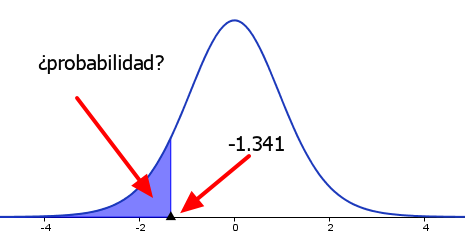
\includegraphics[width=10cm]{../fig/Tut06-20.png}
  \end{center}


  \item
  Se puede hacer de dos formas:
\begin{knitrout}
\definecolor{shadecolor}{rgb}{0.969, 0.969, 0.969}\color{fgcolor}\begin{kframe}
\begin{alltt}
\hlnum{1} \hlopt{-} \hlkwd{pt}\hlstd{(}\hlnum{2.602}\hlstd{,} \hlkwc{df}\hlstd{=k)}
\end{alltt}
\begin{verbatim}
## [1] 0.01001
\end{verbatim}
\begin{alltt}
\hlkwd{pt}\hlstd{(}\hlnum{2.602}\hlstd{,} \hlkwc{df}\hlstd{=k,} \hlkwc{lower.tail}\hlstd{=}\hlnum{FALSE}\hlstd{)}
\end{alltt}
\begin{verbatim}
## [1] 0.01001
\end{verbatim}
\end{kframe}
\end{knitrout}
  \begin{center}
        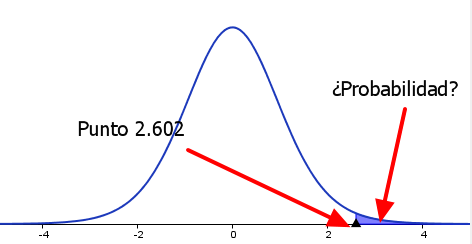
\includegraphics[width=10cm]{../fig/Tut06-21.png}
  \end{center}

  \item
\begin{knitrout}
\definecolor{shadecolor}{rgb}{0.969, 0.969, 0.969}\color{fgcolor}\begin{kframe}
\begin{alltt}
\hlkwd{pt}\hlstd{(}\hlnum{1.753}\hlstd{,} \hlkwc{df}\hlstd{=k)} \hlopt{-} \hlkwd{pt}\hlstd{(}\hlopt{-}\hlnum{1.753}\hlstd{,} \hlkwc{df}\hlstd{=k)}
\end{alltt}
\begin{verbatim}
## [1] 0.89999
\end{verbatim}
\end{kframe}
\end{knitrout}
  \begin{center}
        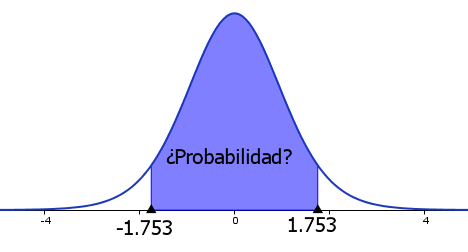
\includegraphics[width=10cm]{../fig/Tut06-22.png}
  \end{center}

  \item
\begin{knitrout}
\definecolor{shadecolor}{rgb}{0.969, 0.969, 0.969}\color{fgcolor}\begin{kframe}
\begin{alltt}
\hlkwd{qt}\hlstd{(}\hlnum{0.95}\hlstd{,} \hlkwc{df}\hlstd{=k)}
\end{alltt}
\begin{verbatim}
## [1] 1.7531
\end{verbatim}
\end{kframe}
\end{knitrout}
  \begin{center}
        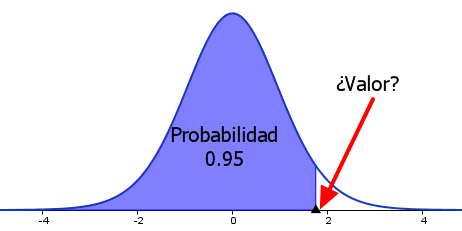
\includegraphics[width=10cm]{../fig/Tut06-23.png}
  \end{center}
  ¿Ves la relación con el apartado anterior? En el apartado anterior las dos colas suman $0.1$. Así que. ¿cuál es el área de cada una de las colas? ¿Y cuál es el área de la cola derecha en la figura de este apartado?

  \item
  De dos formas:
\begin{knitrout}
\definecolor{shadecolor}{rgb}{0.969, 0.969, 0.969}\color{fgcolor}\begin{kframe}
\begin{alltt}
\hlkwd{qt}\hlstd{(}\hlnum{0.025}\hlstd{,} \hlkwc{df}\hlstd{=k,} \hlkwc{lower.tail}\hlstd{=}\hlnum{FALSE}\hlstd{)}
\end{alltt}
\begin{verbatim}
## [1] 2.1314
\end{verbatim}
\begin{alltt}
\hlkwd{qt}\hlstd{(}\hlnum{1} \hlopt{-} \hlnum{0.025}\hlstd{,} \hlkwc{df}\hlstd{=k)}
\end{alltt}
\begin{verbatim}
## [1] 2.1314
\end{verbatim}
\end{kframe}
\end{knitrout}
  En el segundo método fíjate en que siempre que usamos el truco de {\em restar de $1$}, lo que restamos tiene que ser una probabilidad $p$, de forma que hacemos $1 - p$. Cuando usamos {\tt qt} la probabilidad está {\em dentro} de la función, y por eso expresiones como {\tt qt(1-p, ...)} tienen sentido. En cambio, una expresión como {\tt 1 - qt(...)} es, casi siempre, el resultado de un error de interpretación.
  \begin{center}
        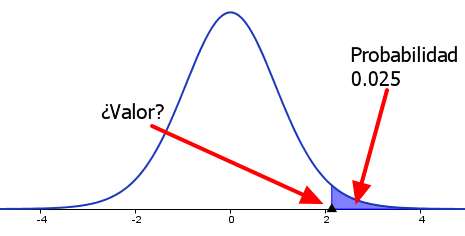
\includegraphics[width=10cm]{../fig/Tut06-24.png}
  \end{center}


  \item
\begin{knitrout}
\definecolor{shadecolor}{rgb}{0.969, 0.969, 0.969}\color{fgcolor}\begin{kframe}
\begin{alltt}
\hlkwd{qt}\hlstd{(}\hlnum{0.05}\hlstd{,} \hlkwc{df}\hlstd{=k)}
\end{alltt}
\begin{verbatim}
## [1] -1.7531
\end{verbatim}
\end{kframe}
\end{knitrout}
  El resultado es el opuesto del que obtuvimos en el apartado 4, y la figura debería dejar claro por qué es así. ¿Cuánto vale la cola derecha en la figura del apartado 4?
  \begin{center}
        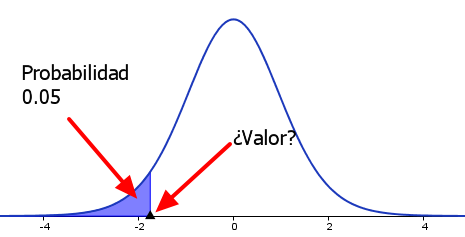
\includegraphics[width=10cm]{../fig/Tut06-25.png}
  \end{center}

  \item
  De dos formas:
\begin{knitrout}
\definecolor{shadecolor}{rgb}{0.969, 0.969, 0.969}\color{fgcolor}\begin{kframe}
\begin{alltt}
\hlkwd{qt}\hlstd{(}\hlnum{0.975}\hlstd{,} \hlkwc{df}\hlstd{=k,} \hlkwc{lower.tail}\hlstd{=}\hlnum{FALSE}\hlstd{)}
\end{alltt}
\begin{verbatim}
## [1] -2.1314
\end{verbatim}
\begin{alltt}
\hlkwd{qt}\hlstd{(}\hlnum{1}\hlopt{-} \hlnum{0.975}\hlstd{,} \hlkwc{df}\hlstd{=k)}
\end{alltt}
\begin{verbatim}
## [1] -2.1314
\end{verbatim}
\end{kframe}
\end{knitrout}
  \begin{center}
        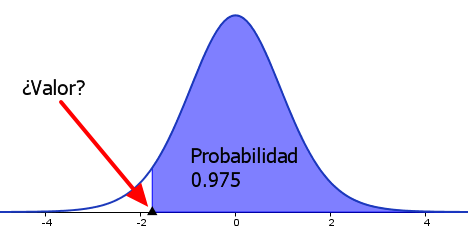
\includegraphics[width=10cm]{../fig/Tut06-26.png}
  \end{center}
  La relación con el apartados 5 debe estar clara a estas alturas.

  \item
  Este apartado es el más directamente se relaciona con la construcción de los intervalos de confianza. Y en este caso es mejor empezar por la figura.
  \begin{center}
        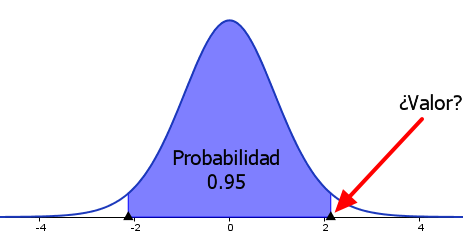
\includegraphics[width=10cm]{../fig/Tut06-27.png}
  \end{center}
  Como muestra la figura, el área conjunta de las dos colas debe ser igual a $1-0.95=0.05$. Así que el área de la cola derecha no sombreada es 0.025. Y eso demuestra que el valor que buscamos es, por tanto, el que mismo que hemos calculado en el anterior apartado.

  \item Dejamos la figura de este apartado al lector, es muy parecida a la del anterior, cambiando sólo los valores numéricos. En cualquier caso, la suma conjunta de las dos colas es, en este apartado, $1 - 0.93 = 0.07$. Por lo tanto la cola derecha vale $0.035$. Y entonces el valor se obtiene con
\begin{knitrout}
\definecolor{shadecolor}{rgb}{0.969, 0.969, 0.969}\color{fgcolor}\begin{kframe}
\begin{alltt}
\hlkwd{qt}\hlstd{(}\hlnum{0.035}\hlstd{,} \hlkwc{df}\hlstd{=k,} \hlkwc{lower.tail}\hlstd{=}\hlnum{FALSE}\hlstd{)}
\end{alltt}
\begin{verbatim}
## [1] 1.9509
\end{verbatim}
\begin{alltt}
\hlkwd{qt}\hlstd{(}\hlnum{1}\hlopt{-} \hlnum{0.035}\hlstd{,} \hlkwc{df}\hlstd{=k)}
\end{alltt}
\begin{verbatim}
## [1] 1.9509
\end{verbatim}
\end{kframe}
\end{knitrout}

\end{enumerate}


\paragraph{\bf $\bullet$ Ejercicio \ref{tut06:ejercicio11}, pág. \pageref{tut06:ejercicio11}}
\label{tut06:ejercicio11:sol}\quad\\

En R, el primer valor se obtiene de una de estas dos maneras:
\begin{knitrout}
\definecolor{shadecolor}{rgb}{0.969, 0.969, 0.969}\color{fgcolor}\begin{kframe}
\begin{alltt}
\hlkwd{pt}\hlstd{(}\hlnum{2.3}\hlstd{,} \hlkwc{df}\hlstd{=}\hlnum{21}\hlstd{,} \hlkwc{lower.tail}\hlstd{=}\hlnum{FALSE}\hlstd{)}
\end{alltt}
\begin{verbatim}
## [1] 0.015901
\end{verbatim}
\begin{alltt}
\hlnum{1} \hlopt{-} \hlkwd{pt}\hlstd{(}\hlnum{2.3}\hlstd{,} \hlkwc{df}\hlstd{=}\hlnum{21}\hlstd{)}
\end{alltt}
\begin{verbatim}
## [1] 0.015901
\end{verbatim}
\end{kframe}
\end{knitrout}
Y el segundo mediante:
\begin{knitrout}
\definecolor{shadecolor}{rgb}{0.969, 0.969, 0.969}\color{fgcolor}\begin{kframe}
\begin{alltt}
\hlkwd{pt}\hlstd{(}\hlnum{2.3}\hlstd{,} \hlkwc{df}\hlstd{=}\hlnum{12}\hlstd{)} \hlopt{-} \hlkwd{pt}\hlstd{(}\hlopt{-}\hlnum{1.2}\hlstd{,} \hlkwc{df}\hlstd{=}\hlnum{12}\hlstd{)}
\end{alltt}
\begin{verbatim}
## [1] 0.85325
\end{verbatim}
\end{kframe}
\end{knitrout}


En GeoGebra, para el primer valor puedes usar la {\em Calculadora de Probabilidades}, o más directamente el comando:
\begin{verbatim}
  1 - DistribuciónT[21, 2.3]
\end{verbatim}
Para el segundo valor usaríamos:
\begin{verbatim}
  DistribuciónT[12, 2.3] - DistribuciónT[12, -1.2]
\end{verbatim}


\paragraph{\bf $\bullet$ Ejercicio \ref{tut06:ejercicio12}, pág. \pageref{tut06:ejercicio12}}
\label{tut06:ejercicio12:sol}\quad\\

En R, de cualquiera de estas maneras:
\begin{knitrout}
\definecolor{shadecolor}{rgb}{0.969, 0.969, 0.969}\color{fgcolor}\begin{kframe}
\begin{alltt}
\hlkwd{qt}\hlstd{(}\hlnum{0.93}\hlstd{,} \hlkwc{df}\hlstd{=}\hlnum{12}\hlstd{)}
\end{alltt}
\begin{verbatim}
## [1] 1.5804
\end{verbatim}
\begin{alltt}
\hlkwd{qt}\hlstd{(}\hlnum{0.07}\hlstd{,} \hlkwc{df}\hlstd{=}\hlnum{12}\hlstd{,} \hlkwc{lower.tail}\hlstd{=}\hlnum{FALSE}\hlstd{)}
\end{alltt}
\begin{verbatim}
## [1] 1.5804
\end{verbatim}
\end{kframe}
\end{knitrout}
En GeoGebra con:
\begin{verbatim}
  DistribuciónTInversa[12, 0.93]
\end{verbatim}


\paragraph{\bf $\bullet$ Ejercicio \ref{tut06:ejercicio13}, pág. \pageref{tut06:ejercicio13}}
\label{tut06:ejercicio13:sol}\quad\\

\begin{enumerate}
  \item Como se explica en la página que sigue al enunciado de este ejercicio, la función {\tt DISTR.T} de Calc, con {\tt modo = 1}, usa la cola derecha de la distribución $t$ de Student.
  \item En R puedes calcular ese valor con:
\begin{knitrout}
\definecolor{shadecolor}{rgb}{0.969, 0.969, 0.969}\color{fgcolor}\begin{kframe}
\begin{alltt}
\hlkwd{pt}\hlstd{(}\hlnum{0.5}\hlstd{,} \hlkwc{df}\hlstd{=}\hlnum{3}\hlstd{,} \hlkwc{lower.tail}\hlstd{=}\hlnum{FALSE}\hlstd{)}
\end{alltt}
\begin{verbatim}
## [1] 0.32572
\end{verbatim}
\end{kframe}
\end{knitrout}

\end{enumerate}

\paragraph{\bf $\bullet$ Ejercicio \ref{tut06:ejercicio14}, pág. \pageref{tut06:ejercicio14}}
\label{tut06:ejercicio14:sol}\quad\\

\begin{enumerate}
  \item El intervalo es $\mu =  132.5\pm 1.645$ o, de otro modo:
    \[ 130.9 < \mu < 134.1\]

  \item El intervalo es $\mu = 3.192 \pm 0.4604$ o, de otro modo:
  \[ 2.732  < \mu < 3.652\]
  El valor $\bar X = 3.192$ se obtiene como parte de la salida del programa.

  \item Después de elegir el directorio de trabajo (el que contiene el fichero), en el paso 2 hemos usado la función {\tt read.table} así:
        \begin{verbatim}
          muestra = read.table(file="../datos/Tut06-DatosIntConfConStudent.csv",
          header=FALSE, sep=" ",dec=",")[,1]
        \end{verbatim}

  El intervalo es $\mu = 3.5 \pm 0.5616$ o, de otro modo:
  \[ 2.939  < \mu < 4.062\]
  De nuevo, el valor $\bar X = 3.5$ se obtiene como parte de la salida del programa.

  \item Al usar la $t$ de Student con $n=450$ (y por tanto $449$ grados de libertad) se obtiene un intervalo de confianza con semianchura {\tt 0.2805}, frente a la semianchura {\tt 0.2793} que se obtuvo en el Ejercicio usando $Z$. La diferencia entre los dos intervalos es del orden de milésimas, así que son prácticamente iguales. Este ejercicio indica que si usamos la $t$ de Student en lugar de $Z$ cuando las muestras son grandes, los resultados serán muy parecidos.

\item Mostramos aquí el código correspondiente al intervalo al $95\%$. Es simplemente, el fichero plantilla {\tt Tut06-IntConf-Media-UsandoT-Estadisticos.R}, del que hemos eliminado los comentarios introductorios y las instrucciones. Para hallar el intervalo al $99\%$ sólo hay que cambiar  una línea del código.
\begin{knitrout}
\definecolor{shadecolor}{rgb}{0.969, 0.969, 0.969}\color{fgcolor}\begin{kframe}
\begin{alltt}
\hlcom{# Introduce el numero de datos de la muestra,}
\hlstd{n} \hlkwb{=} \hlnum{10}

\hlcom{# Introduce aqui el valor de xbar, la media muestral}
\hlstd{xbar} \hlkwb{=} \hlnum{2.35}

\hlcom{# Cuasidesviacion tipica muestral}
\hlstd{s} \hlkwb{=} \hlnum{0.61}

\hlcom{# y el nivel de confianza deseado.}
\hlstd{nc} \hlkwb{=} \hlnum{0.95}

\hlcom{################################################}
\hlcom{#NO CAMBIES NADA DE AQUI PARA ABAJO}
\hlcom{################################################}
\hlstd{(alfa} \hlkwb{=} \hlnum{1} \hlopt{-} \hlstd{nc )}
\end{alltt}
\begin{verbatim}
## [1] 0.05
\end{verbatim}
\begin{alltt}
\hlcom{# Calculamos el valor critico:}

\hlstd{(t_alfa2} \hlkwb{=} \hlkwd{qt}\hlstd{(} \hlnum{1} \hlopt{-} \hlstd{alfa} \hlopt{/} \hlnum{2} \hlstd{,} \hlkwc{df}\hlstd{=n}\hlopt{-}\hlnum{1} \hlstd{) )}
\end{alltt}
\begin{verbatim}
## [1] 2.2622
\end{verbatim}
\begin{alltt}
\hlcom{#y la semianchura del intervalo}
\hlstd{(semianchura}\hlkwb{=}\hlstd{t_alfa2} \hlopt{*} \hlstd{s} \hlopt{/} \hlkwd{sqrt}\hlstd{(n) )}
\end{alltt}
\begin{verbatim}
## [1] 0.43637
\end{verbatim}
\begin{alltt}
\hlcom{# Y el intervalo de confianza (a,b) para mu es este:}
\hlstd{xbar} \hlopt{+} \hlkwd{c}\hlstd{(}\hlopt{-}\hlnum{1}\hlstd{,} \hlnum{1}\hlstd{)} \hlopt{*} \hlstd{semianchura}
\end{alltt}
\begin{verbatim}
## [1] 1.9136 2.7864
\end{verbatim}
\end{kframe}
\end{knitrout}


\end{enumerate}

\paragraph{\bf $\bullet$ Ejercicio \ref{tut06:ejercicio15}, pág. \pageref{tut06:ejercicio15}}
\label{tut06:ejercicio15:sol}\quad\\

Asegúrate, usando por ejemplo {\tt setwd}, de que el directorio de trabajo (en mi caso, es el {\em Escritorio}) es el que contiene el fichero de datos {\tt Tut06-DatosIntConfConStudent.csv}. Entonces leemos los datos en un vector {\tt muestra}, como hicimos en el Ejercicio \ref{tut06:ejercicio14}, y aplicamos {\tt t.test}:

\begin{knitrout}
\definecolor{shadecolor}{rgb}{0.969, 0.969, 0.969}\color{fgcolor}\begin{kframe}
\begin{alltt}
\hlstd{muestra} \hlkwb{=} \hlkwd{read.table}\hlstd{(}\hlkwc{file}\hlstd{=}\hlstr{"../datos/Tut06-DatosIntConfConStudent.csv"}\hlstd{,} \hlkwc{sep}\hlstd{=}\hlstr{" "}\hlstd{,} \hlkwc{dec}\hlstd{=}\hlstr{","}\hlstd{)[,}\hlnum{1}\hlstd{]}
\hlstd{T.testMuestra} \hlkwb{=} \hlkwd{t.test}\hlstd{(muestra,} \hlkwc{conf.level}\hlstd{=}\hlnum{0.95}\hlstd{)}
\hlstd{(intervalo} \hlkwb{=} \hlstd{T.testMuestra}\hlopt{$}\hlstd{conf.int)}
\end{alltt}
\begin{verbatim}
## [1] 2.9385 4.0618
## attr(,"conf.level")
## [1] 0.95
\end{verbatim}
\end{kframe}
\end{knitrout}

La respuesta es la misma que en el apartado 3 del Ejercicio \ref{tut06:ejercicio14}.


\paragraph{\bf $\bullet$ Ejercicio \ref{tut06:ejercicio16}, pág. \pageref{tut06:ejercicio16}}
\label{tut06:ejercicio16:sol}\quad\\

\begin{enumerate}
  \item Para el primer apartado ejecutamos:
    \begin{verbatim}
      IntervaloMediaT[ 132.5, 2.3 , 10, 0.95 ]
    \end{verbatim}

  \item Para el segundo, ejecutamos, consecutivamente:
  {\footnotesize
  \begin{verbatim}
datos = {3.14, 3.71, 2.77, 4.08, 4.18, 1.51, 3.65, 3.41, 4.51, 2.27, 3.28,2.26, 2.80, 2.54, 3.77}
IntervaloMediaT[datos, 0.95 ]
  \end{verbatim}
  }

\end{enumerate}


\paragraph{\bf $\bullet$ Ejercicio \ref{tut06:ejercicio17}, pág. \pageref{tut06:ejercicio17}}
\label{tut06:ejercicio17:sol}\quad\\

\begin{enumerate}
  \item La probabilidad es aproximadamente  $0.01$.\quad\\
    \begin{center}
    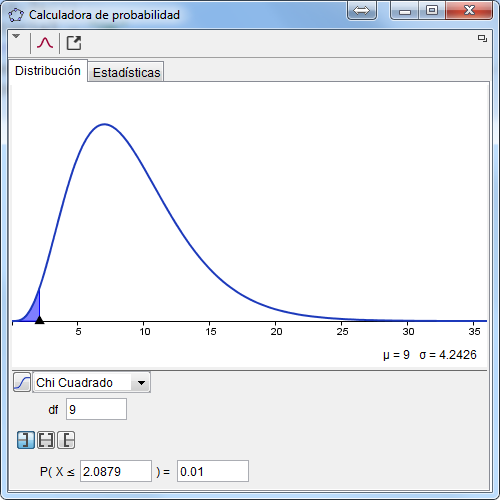
\includegraphics[width=8cm]{../fig/Tut06-30.png}
    \end{center}
  \item La probabilidad es aproximadamente  $0.2493$.\quad\\
    \begin{center}
    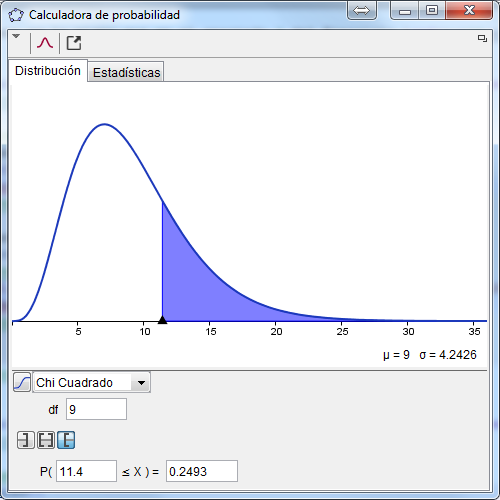
\includegraphics[width=8cm]{../fig/Tut06-31.png}
    \end{center}
  \item La probabilidad es aproximadamente  $0.0492$.\quad\\
    \begin{center}
    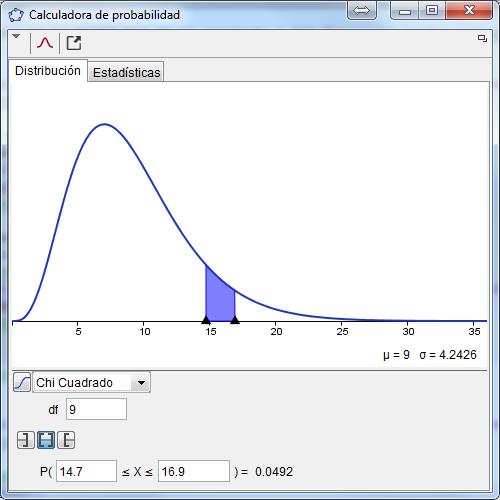
\includegraphics[width=10cm]{../fig/Tut06-32.png}
    \end{center}
  \item El valor es aproximadamente  $16.919$. \quad\\
    \begin{center}
    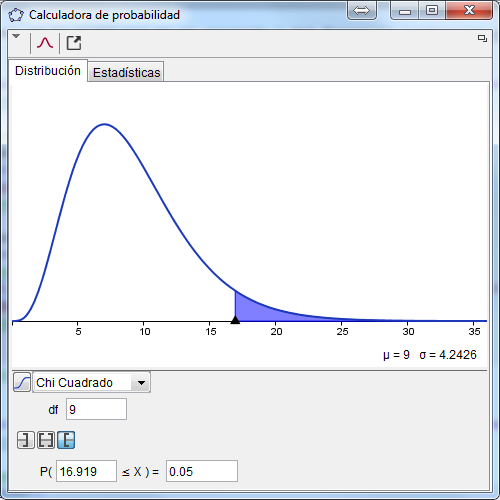
\includegraphics[width=10cm]{../fig/Tut06-33.png}
    \end{center}

\newpage

  \item El valor es aproximadamente $2.0879$\quad\\
    \begin{center}
    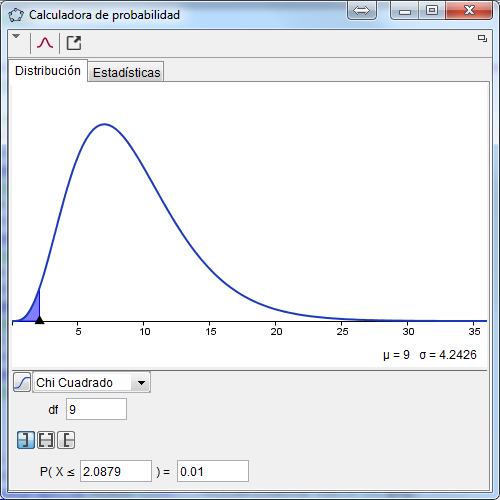
\includegraphics[width=12cm]{../fig/Tut06-34.png}
    \end{center}

  \item El último apartado es el más difícil, a causa de la falta de simetría. Como ilustra la siguiente figura, nuestro objetivo es conseguir que la zona central sombreada, que corresponde a la probabilidad $P(y_1 < Y < y_2)$, tenga un área igual a $0.90$. Eso significa que las dos colas suman $0.10$. Pero como además, son iguales (es esencial saber esto, porque no hay simetría), eso significa que cada una de ellas vale $0.05$.
    \begin{center}
    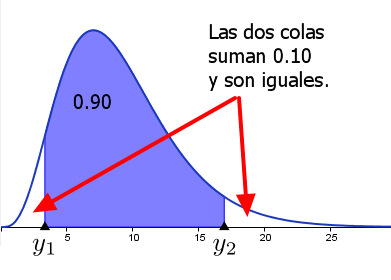
\includegraphics[width=12cm]{../fig/Tut06-35.png}
    \end{center}
    En particular eso implica que:
    \[P(Y < y_2) = 0.90 + 0.05 = 0.95\]
    y que:
    \[P(Y < y_1) =  0.05\]
    Ahora es fácil proceder como en el apartado 1 para obtener $y_1 = 3.3251$ e $y_2=16.919$. ¿Ves la relación entre $y_2$ y el apartado 4 de este ejercicio? ¿Y ves también que no hay ningún tipo de simetría entre $y_1$ e $y_2$?

\end{enumerate}

\paragraph{\bf $\bullet$ Ejercicio \ref{tut06:ejercicio18}, pág. \pageref{tut06:ejercicio18}}
\label{tut06:ejercicio18:sol}\quad\\
Usa el menú {\em Opciones} de GeoGebra para ver más cifras decimales si es necesario.
\begin{itemize}
    \item[] Apartado 2:
        \begin{verbatim}
        1- ChiCuadrado[9, 11.4]
        \end{verbatim}
    \item[]Apartado 3:
        \begin{verbatim}
        ChiCuadrado[9, 16.9] - ChiCuadrado[9, 14.7]
        \end{verbatim}
    \item[]Apartado 4: (Atención a la posición del $1 - p$).
        \begin{verbatim}
        ChiCuadradoInversa[9, 1- 0.05]
        \end{verbatim}
    \item[]Apartado 6: El valor $y_1$ se obtiene con:\\
        \begin{verbatim}
        ChiCuadradoInversa[9, 0.05]
        \end{verbatim}
        \qquad mientras que el valor $y_2$ se obtiene con:
        \begin{verbatim}
        ChiCuadradoInversa[9, 0.95]
        \end{verbatim}
\end{itemize}

\paragraph{\bf $\bullet$ Ejercicio \ref{tut06:ejercicio19}, pág. \pageref{tut06:ejercicio19}}
\label{tut06:ejercicio19:sol}\quad\\

\begin{enumerate}
  \item Código del apartado 1:
\begin{knitrout}
\definecolor{shadecolor}{rgb}{0.969, 0.969, 0.969}\color{fgcolor}\begin{kframe}
\begin{alltt}
\hlcom{# Fijamos los grados de libertad:}

\hlstd{k} \hlkwb{=} \hlnum{9}

\hlcom{# Apartado 1}

\hlkwd{pchisq}\hlstd{(}\hlnum{2.09}\hlstd{,} \hlkwc{df}\hlstd{=k)}
\end{alltt}
\begin{verbatim}
## [1] 0.010037
\end{verbatim}
\begin{alltt}
\hlcom{# Apartado 2}

\hlnum{1} \hlopt{-} \hlkwd{pchisq}\hlstd{(}\hlnum{11.4}\hlstd{,} \hlkwc{df}\hlstd{=k)}
\end{alltt}
\begin{verbatim}
## [1] 0.24928
\end{verbatim}
\begin{alltt}
\hlkwd{pchisq}\hlstd{(}\hlnum{11.4}\hlstd{,} \hlkwc{df}\hlstd{=k,} \hlkwc{lower.tail}\hlstd{=}\hlnum{FALSE}\hlstd{)}
\end{alltt}
\begin{verbatim}
## [1] 0.24928
\end{verbatim}
\begin{alltt}
\hlcom{# Apartado 3}

\hlkwd{pchisq}\hlstd{(}\hlnum{16.9}\hlstd{,} \hlkwc{df}\hlstd{=k)} \hlopt{-} \hlkwd{pchisq}\hlstd{(}\hlnum{14.7}\hlstd{,} \hlkwc{df}\hlstd{=k)}
\end{alltt}
\begin{verbatim}
## [1] 0.049208
\end{verbatim}
\begin{alltt}
\hlcom{# Apartado 4}

\hlkwd{qchisq}\hlstd{(}\hlnum{1} \hlopt{-} \hlnum{0.05}\hlstd{,} \hlkwc{df}\hlstd{=k)}
\end{alltt}
\begin{verbatim}
## [1] 16.919
\end{verbatim}
\begin{alltt}
\hlkwd{qchisq}\hlstd{(}\hlnum{0.05}\hlstd{,} \hlkwc{df}\hlstd{=k,} \hlkwc{lower.tail}\hlstd{=}\hlnum{FALSE}\hlstd{)}
\end{alltt}
\begin{verbatim}
## [1] 16.919
\end{verbatim}
\begin{alltt}
\hlcom{# Apartado 5}

\hlkwd{qchisq}\hlstd{(}\hlnum{0.01}\hlstd{,} \hlkwc{df}\hlstd{=k)}
\end{alltt}
\begin{verbatim}
## [1] 2.0879
\end{verbatim}
\begin{alltt}
\hlcom{# Apartado 6}

\hlcom{# y1 se obtiene con}

\hlkwd{qchisq}\hlstd{(}\hlnum{0.05}\hlstd{,} \hlkwc{df}\hlstd{=k)}
\end{alltt}
\begin{verbatim}
## [1] 3.3251
\end{verbatim}
\begin{alltt}
\hlcom{# mientras que y2 se obtiene con}

\hlkwd{qchisq}\hlstd{(}\hlnum{0.95}\hlstd{,} \hlkwc{df}\hlstd{=k)}
\end{alltt}
\begin{verbatim}
## [1] 16.919
\end{verbatim}
\end{kframe}
\end{knitrout}

  \item Código del apartado 2:
        El valor $a$ que cumple
        \[P(\chi^2_4 < a) = 0.05\]
        es:
\begin{knitrout}
\definecolor{shadecolor}{rgb}{0.969, 0.969, 0.969}\color{fgcolor}\begin{kframe}
\begin{alltt}
\hlkwd{qchisq}\hlstd{(}\hlnum{0.05}\hlstd{,} \hlkwc{df}\hlstd{=}\hlnum{4}\hlstd{)}
\end{alltt}
\begin{verbatim}
## [1] 0.71072
\end{verbatim}
\end{kframe}
\end{knitrout}
        y el valor $b$ que cumple
        \[P(\chi^2_4 > b) = 0.05\]
        se calcula de una de estas dos formas:
\begin{knitrout}
\definecolor{shadecolor}{rgb}{0.969, 0.969, 0.969}\color{fgcolor}\begin{kframe}
\begin{alltt}
\hlkwd{qchisq}\hlstd{(}\hlnum{1} \hlopt{-} \hlnum{0.05}\hlstd{,} \hlkwc{df}\hlstd{=}\hlnum{4}\hlstd{)}
\end{alltt}
\begin{verbatim}
## [1] 9.4877
\end{verbatim}
\begin{alltt}
\hlkwd{qchisq}\hlstd{(}\hlnum{0.05}\hlstd{,} \hlkwc{df}\hlstd{=}\hlnum{4}\hlstd{,} \hlkwc{lower.tail}\hlstd{=}\hlnum{FALSE}\hlstd{)}
\end{alltt}
\begin{verbatim}
## [1] 9.4877
\end{verbatim}
\end{kframe}
\end{knitrout}

\end{enumerate}


\paragraph{\bf $\bullet$ Ejercicio \ref{tut06:ejercicio20}, pág. \pageref{tut06:ejercicio20}}
\label{tut06:ejercicio20:sol}\quad\\


En R, para el primer ejemplo hacemos:
\begin{knitrout}
\definecolor{shadecolor}{rgb}{0.969, 0.969, 0.969}\color{fgcolor}\begin{kframe}
\begin{alltt}
\hlkwd{pchisq}\hlstd{(}\hlnum{15}\hlstd{,} \hlkwc{df}\hlstd{=}\hlnum{12}\hlstd{)} \hlopt{-} \hlkwd{pchisq}\hlstd{(}\hlnum{10}\hlstd{,} \hlkwc{df}\hlstd{=}\hlnum{12}\hlstd{)}
\end{alltt}
\begin{verbatim}
## [1] 0.37452
\end{verbatim}
\end{kframe}
\end{knitrout}
y para el segundo, uno de estos comandos:
\begin{knitrout}
\definecolor{shadecolor}{rgb}{0.969, 0.969, 0.969}\color{fgcolor}\begin{kframe}
\begin{alltt}
\hlkwd{qchisq}\hlstd{(}\hlnum{7}\hlopt{/}\hlnum{13}\hlstd{,} \hlkwc{df}\hlstd{=}\hlnum{7}\hlstd{,} \hlkwc{lower.tail}\hlstd{=}\hlnum{FALSE}\hlstd{)}
\end{alltt}
\begin{verbatim}
## [1] 6.011
\end{verbatim}
\begin{alltt}
\hlkwd{qchisq}\hlstd{(}\hlnum{1} \hlopt{-} \hlstd{(}\hlnum{7}\hlopt{/}\hlnum{13}\hlstd{),} \hlkwc{df}\hlstd{=}\hlnum{7}\hlstd{)}
\end{alltt}
\begin{verbatim}
## [1] 6.011
\end{verbatim}
\end{kframe}
\end{knitrout}

En GeoGebra, para el primero ejecuta en la {\em Línea de Entrada}:
\begin{verbatim}
ChiCuadrado[12, 15] - ChiCuadrado[12, 10]
\end{verbatim}
y para el segundo:
\begin{verbatim}
ChiCuadradoInversa[7, 1 - (7/13)]
\end{verbatim}

\paragraph{\bf $\bullet$ Ejercicio \ref{tut06:ejercicio21}, pág. \pageref{tut06:ejercicio21}}
\label{tut06:ejercicio21:sol}\quad\\

El código es este:
\begin{knitrout}
\definecolor{shadecolor}{rgb}{0.969, 0.969, 0.969}\color{fgcolor}\begin{kframe}
\begin{alltt}
\hlstd{n} \hlkwb{=} \hlnum{30}
\hlstd{k} \hlkwb{=} \hlstd{n} \hlopt{-} \hlnum{1}
\hlstd{s} \hlkwb{=} \hlnum{2.6}

\hlstd{nc} \hlkwb{=} \hlnum{0.95}
\hlstd{(alfa} \hlkwb{=} \hlnum{1} \hlopt{-} \hlstd{nc)}
\end{alltt}
\begin{verbatim}
## [1] 0.05
\end{verbatim}
\begin{alltt}
\hlstd{(alfa2} \hlkwb{=} \hlstd{alfa} \hlopt{/}\hlnum{2}\hlstd{)}
\end{alltt}
\begin{verbatim}
## [1] 0.025
\end{verbatim}
\begin{alltt}
\hlstd{(chiAlfa2} \hlkwb{=} \hlkwd{qchisq}\hlstd{(}\hlnum{1} \hlopt{-} \hlstd{alfa2,} \hlkwc{df}\hlstd{=k))}
\end{alltt}
\begin{verbatim}
## [1] 45.722
\end{verbatim}
\begin{alltt}
\hlstd{(chiUnoMenosAlfa2} \hlkwb{=} \hlkwd{qchisq}\hlstd{(alfa2,} \hlkwc{df}\hlstd{=k))}
\end{alltt}
\begin{verbatim}
## [1] 16.047
\end{verbatim}
\begin{alltt}
\hlstd{(intervalo} \hlkwb{=} \hlstd{s} \hlopt{*} \hlkwd{sqrt}\hlstd{(k} \hlopt{/} \hlkwd{c}\hlstd{(chiAlfa2, chiUnoMenosAlfa2)))}
\end{alltt}
\begin{verbatim}
## [1] 2.0707 3.4952
\end{verbatim}
\end{kframe}
\end{knitrout}

\paragraph{\bf $\bullet$ Ejercicio \ref{tut06:ejercicio22}, pág. \pageref{tut06:ejercicio22}}
\label{tut06:ejercicio22:sol}\quad\\

Para el segundo apartado, el código del fichero con los datos de ese apartado es este:
\begin{knitrout}
\definecolor{shadecolor}{rgb}{0.969, 0.969, 0.969}\color{fgcolor}\begin{kframe}
\begin{alltt}
\hlcom{# Introducimos el valor de la desviacion tipica muestral,}
\hlstd{s} \hlkwb{=} \hlnum{2.81}

\hlcom{# el tamaño de la muestra,}
\hlstd{n} \hlkwb{=} \hlnum{87}

\hlcom{# y el nivel de confianza deseado.}
\hlstd{nc} \hlkwb{=} \hlnum{0.95}

\hlcom{################################################}
\hlcom{#NO CAMBIES NADA DE AQUI PARA ABAJO}
\hlcom{################################################}
\hlcom{# Calculamos alfa}
\hlstd{(alfa} \hlkwb{=} \hlnum{1} \hlopt{-} \hlstd{nc)}
\end{alltt}
\begin{verbatim}
## [1] 0.05
\end{verbatim}
\begin{alltt}
\hlstd{(alfa2} \hlkwb{=} \hlstd{alfa} \hlopt{/} \hlnum{2}\hlstd{)}
\end{alltt}
\begin{verbatim}
## [1] 0.025
\end{verbatim}
\begin{alltt}
\hlcom{# y los grados de libertad:}

\hlstd{(k}\hlkwb{=} \hlstd{n} \hlopt{-} \hlnum{1}\hlstd{)}
\end{alltt}
\begin{verbatim}
## [1] 86
\end{verbatim}
\begin{alltt}
\hlcom{# Calculamos los valores criticos necesarios:}

\hlstd{(chiAlfa2} \hlkwb{=} \hlkwd{qchisq}\hlstd{(}\hlnum{1} \hlopt{-} \hlstd{(alfa}\hlopt{/}\hlnum{2}\hlstd{),} \hlkwc{df}\hlstd{=k))}
\end{alltt}
\begin{verbatim}
## [1] 113.54
\end{verbatim}
\begin{alltt}
\hlstd{(chiUnoMenosAlfa2} \hlkwb{=} \hlkwd{qchisq}\hlstd{(alfa}\hlopt{/}\hlnum{2}\hlstd{,} \hlkwc{df}\hlstd{=k))}
\end{alltt}
\begin{verbatim}
## [1] 62.239
\end{verbatim}
\begin{alltt}
\hlcom{#Para la varianza, el intervalo de confianza sera}
\hlcom{# extremo inferior}
\hlstd{(intervaloVar} \hlkwb{=} \hlstd{s}\hlopt{^}\hlnum{2} \hlopt{*} \hlstd{k} \hlopt{/} \hlkwd{c}\hlstd{(chiAlfa2, chiUnoMenosAlfa2))}
\end{alltt}
\begin{verbatim}
## [1]  5.9807 10.9107
\end{verbatim}
\begin{alltt}
\hlcom{# Y para la desviacion tipica el intervalo de confianza es este:}
\hlstd{(intervaloS} \hlkwb{=} \hlstd{s} \hlopt{*} \hlkwd{sqrt}\hlstd{(k} \hlopt{/} \hlkwd{c}\hlstd{(chiAlfa2, chiUnoMenosAlfa2)))}
\end{alltt}
\begin{verbatim}
## [1] 2.4455 3.3031
\end{verbatim}
\end{kframe}
\end{knitrout}
Para el tercer apartado, fijamos el directorio de trabajo (en mi caso el {\em Escritorio} de una máquina Windows 7) para que sea el que contiene el fichero de datos, y usamos este código:
{\small

\begin{knitrout}
\definecolor{shadecolor}{rgb}{0.969, 0.969, 0.969}\color{fgcolor}\begin{kframe}
\begin{alltt}
\hlcom{# Una posibilidad es que tengas la muestra como un vector.}
\hlcom{#muestra =   # SI NO SE USA, ESCRIBE # AL PRINCIPIO DE LA LINEA}


\hlcom{# Si lees la muestra de un fichero csv:}
\hlcom{# 1. selecciona el directorio de trabajo}

\hlcom{# 2. Ahora introduce entre las comillas el nombre del fichero, y el tipo de separador, etc.}

\hlcom{# SI NO SE USA, ESCRIBE # AL PRINCIPIO DE LA SIGUIENTE LINEA}
\hlstd{muestra} \hlkwb{=} \hlkwd{read.table}\hlstd{(}\hlkwc{file}\hlstd{=}\hlstr{"../datos/Tut06-datosIntConfDesvTipica.csv"}\hlstd{,} \hlkwc{dec}\hlstd{=}\hlstr{"."}\hlstd{)[ ,}\hlnum{1}\hlstd{]}


\hlcom{# Introducimos el nivel de confianza deseado.}
\hlstd{nc}\hlkwb{=}\hlnum{0.95}

\hlcom{################################################}
\hlcom{#NO CAMBIES NADA DE AQUI PARA ABAJO}
\hlcom{################################################}

\hlcom{# alfa}
\hlstd{(alfa} \hlkwb{=} \hlnum{1} \hlopt{-} \hlstd{nc )}
\end{alltt}
\begin{verbatim}
## [1] 0.05
\end{verbatim}
\begin{alltt}
\hlcom{# Numero de datos de la muestra, grados de libertad}
\hlstd{(n} \hlkwb{=} \hlkwd{length}\hlstd{(muestra))}
\end{alltt}
\begin{verbatim}
## [1] 800
\end{verbatim}
\begin{alltt}
\hlstd{k} \hlkwb{=} \hlstd{n} \hlopt{-} \hlnum{1}

\hlcom{# Cuasidesviacion tipica muestral}
\hlstd{(s} \hlkwb{=} \hlkwd{sd}\hlstd{(muestra))}
\end{alltt}
\begin{verbatim}
## [1] 7.1999
\end{verbatim}
\begin{alltt}
\hlcom{# Calculamos los valores criticos necesarios:}

\hlstd{(chiAlfa2} \hlkwb{=} \hlkwd{qchisq}\hlstd{(}\hlnum{1} \hlopt{-} \hlstd{(alfa}\hlopt{/}\hlnum{2}\hlstd{),} \hlkwc{df}\hlstd{=k))}
\end{alltt}
\begin{verbatim}
## [1] 879.23
\end{verbatim}
\begin{alltt}
\hlstd{(chiUnoMenosAlfa2} \hlkwb{=} \hlkwd{qchisq}\hlstd{(alfa}\hlopt{/}\hlnum{2}\hlstd{,} \hlkwc{df}\hlstd{=k))}
\end{alltt}
\begin{verbatim}
## [1] 722.56
\end{verbatim}
\begin{alltt}
\hlcom{#Para la varianza, el intervalo de confianza sera}
\hlcom{# extremo inferior}
\hlstd{(intervaloVar} \hlkwb{=} \hlstd{s}\hlopt{^}\hlnum{2} \hlopt{*} \hlstd{k} \hlopt{/} \hlkwd{c}\hlstd{(chiAlfa2, chiUnoMenosAlfa2))}
\end{alltt}
\begin{verbatim}
## [1] 47.108 57.322
\end{verbatim}
\begin{alltt}
\hlcom{# Y para la desviacion tipica el intervalo de confianza es este:}
\hlstd{(intervaloS} \hlkwb{=} \hlstd{s} \hlopt{*} \hlkwd{sqrt}\hlstd{(k} \hlopt{/} \hlkwd{c}\hlstd{(chiAlfa2, chiUnoMenosAlfa2)))}
\end{alltt}
\begin{verbatim}
## [1] 6.8635 7.5711
\end{verbatim}
\end{kframe}
\end{knitrout}
}




\paragraph{\bf $\bullet$ Ejercicio \ref{tut06:ejercicio23}, pág. \pageref{tut06:ejercicio23}}
\label{tut06:ejercicio23:sol}\quad\\

Ejecuta, uno tras otro, estos comandos en la {\em Línea de Entrada} de GeoGebra. Verás que la estructura de la construcción es prácticamente la misma que hemos usado en R, salvo detalles sintácticos de cada programa. El objeto entre llaves en el último comando es una {\em lista} de GeoGebra, y como ves se puede multiplicar listas por números (una especie de {\em ``operación vectorial''}, como las de R, pero {\em a la GeoGebra}).
\begin{verbatim}
n = 17
k = n - 1
s = 2.1
nc = 0.99
alfa = 1 - nc
alfa2 = alfa / 2
chiAlfa2 = ChiCuadradoInversa[k, 1 - alfa2]
chiUnoMenosAlfa2 = ChiCuadradoInversa[k, alfa2]
intervalo = s * {sqrt(k / chiAlfa2),   sqrt(k / chiUnoMenosAlfa2) }
\end{verbatim}

\paragraph{\bf $\bullet$ Ejercicio \ref{tut06:ejercicio24}, pág. \pageref{tut06:ejercicio24}}
\label{tut06:ejercicio24:sol}\quad\\
Ejecutamos el código sin fijar el valor de {\tt sigma} (recuerda fijar el directorio de trabajo), y el resultado es erróneo.
\begin{knitrout}
\definecolor{shadecolor}{rgb}{0.969, 0.969, 0.969}\color{fgcolor}\begin{kframe}
\begin{alltt}
\hlstd{muestra} \hlkwb{=} \hlkwd{read.table}\hlstd{(}\hlkwc{file}\hlstd{=}\hlstr{"../datos/Tut06-IntConf-Media-UsandoZ-datos.csv"}\hlstd{,} \hlkwc{sep}\hlstd{=}\hlstr{" "}\hlstd{,} \hlkwc{dec}\hlstd{=}\hlstr{"."}\hlstd{)[,}\hlnum{1}\hlstd{]}
\hlstd{(intAsBio} \hlkwb{=} \hlkwd{ci.mu.z}\hlstd{(}\hlkwc{data}\hlstd{=muestra,} \hlkwc{conf}\hlstd{=}\hlnum{0.95}\hlstd{,} \hlkwc{summarized}\hlstd{=}\hlnum{FALSE}\hlstd{))}
\end{alltt}
\begin{verbatim}
## 
## 95% z Confidence interval for population mean 
## Estimate     2.5%    97.5% 
##   7.2313   7.1436   7.3190
\end{verbatim}
\end{kframe}
\end{knitrout}


\paragraph{\bf $\bullet$ Ejercicio \ref{tut06:ejercicio25}, pág. \pageref{tut06:ejercicio25}}
\label{tut06:ejercicio25:sol}\quad\\

\begin{knitrout}
\definecolor{shadecolor}{rgb}{0.969, 0.969, 0.969}\color{fgcolor}\begin{kframe}
\begin{alltt}
\hlstd{muestra} \hlkwb{=} \hlkwd{read.table}\hlstd{(}\hlkwc{file}\hlstd{=}\hlstr{"../datos/Tut06-datosIntConfDesvTipica.csv"}\hlstd{,} \hlkwc{sep}\hlstd{=}\hlstr{" "}\hlstd{,} \hlkwc{dec}\hlstd{=}\hlstr{"."}\hlstd{)[,}\hlnum{1}\hlstd{]}
\hlstd{(intAsBio} \hlkwb{=} \hlkwd{ci.sigma}\hlstd{(}\hlkwc{data}\hlstd{=muestra,} \hlkwc{conf}\hlstd{=}\hlnum{0.95}\hlstd{,} \hlkwc{summarized}\hlstd{=}\hlnum{FALSE}\hlstd{))}
\end{alltt}
\begin{verbatim}
## 
## 95% Confidence interval for population variance 
## Estimate     2.5%    97.5% 
##   51.838   47.108   57.322
\end{verbatim}
\end{kframe}
\end{knitrout}
El intervalo que hemos obtenido es para la varianza $\sigma^2$. Para obtener un intervalo para $\sigma$ hacemos:
\begin{knitrout}
\definecolor{shadecolor}{rgb}{0.969, 0.969, 0.969}\color{fgcolor}\begin{kframe}
\begin{alltt}
\hlkwd{sqrt}\hlstd{(intAsBio}\hlopt{$}\hlstd{ci[}\hlnum{2}\hlopt{:}\hlnum{3}\hlstd{])}
\end{alltt}
\begin{verbatim}
## [1] 6.8635 7.5711
\end{verbatim}
\end{kframe}
\end{knitrout}
Puedes compararlo con la solución del Ejercicio \ref{tut06:ejercicio22}, que está en la página \pageref{tut06:ejercicio22:sol}.

%#########################################################################################
%#########################################################################################
\vspace{2cm} \hrule
\quad\\
Fin del Tutorial06. ¡Gracias por la atención!

%\newpage
%\addcontentsline{toc}{section}{Guía de trabajo.}
%\includepdf[pages={1-},scale=0.90]{06-GuiaDeTrabajo.pdf}




\end{document}



